% thesis.tex (also saved as simple.tex) -- a simple thesis document
% for demonstrating dalthesis.cls class file, or to use as a starting
% document for writing a thesis.
% If you are not familiar with TeX and LaTeX, the first thing that you
% can learn that line comments start with the percent sign (%), so
% these lines are ignored by the system.  Feel free to change them or
% delete them.
\documentclass[12pt]{report}
\newcommand{\mychapter}[2]{
    \setcounter{chapter}{#1}
    \setcounter{section}{0}
    \chapter*{#2}
    \addcontentsline{toc}{chapter}{#2}
    }
\usepackage[utf8]{inputenc}
\usepackage{graphicx}
\usepackage{gensymb}
\usepackage{comment}
\usepackage{amsmath}
\usepackage{caption}
\usepackage{subcaption}
\usepackage{pdfpages}
\usepackage[toc,page]{appendix}
\usepackage{afterpage}
\usepackage{multirow}


\usepackage[backend=bibtex,style=verbose-trad2]{biblatex}
\bibliography{thesis} 

\newcommand\blankpage{%
    \null
    \thispagestyle{empty}%
    \addtocounter{page}{0}%
    \newpage}
\usepackage{hyperref}

\pagenumbering{roman}



%\renewcommand{\footcite}[1]{\cite{#1}\hypercite{#1}}
\begin{document}


\begin{figure}
 \centering 
 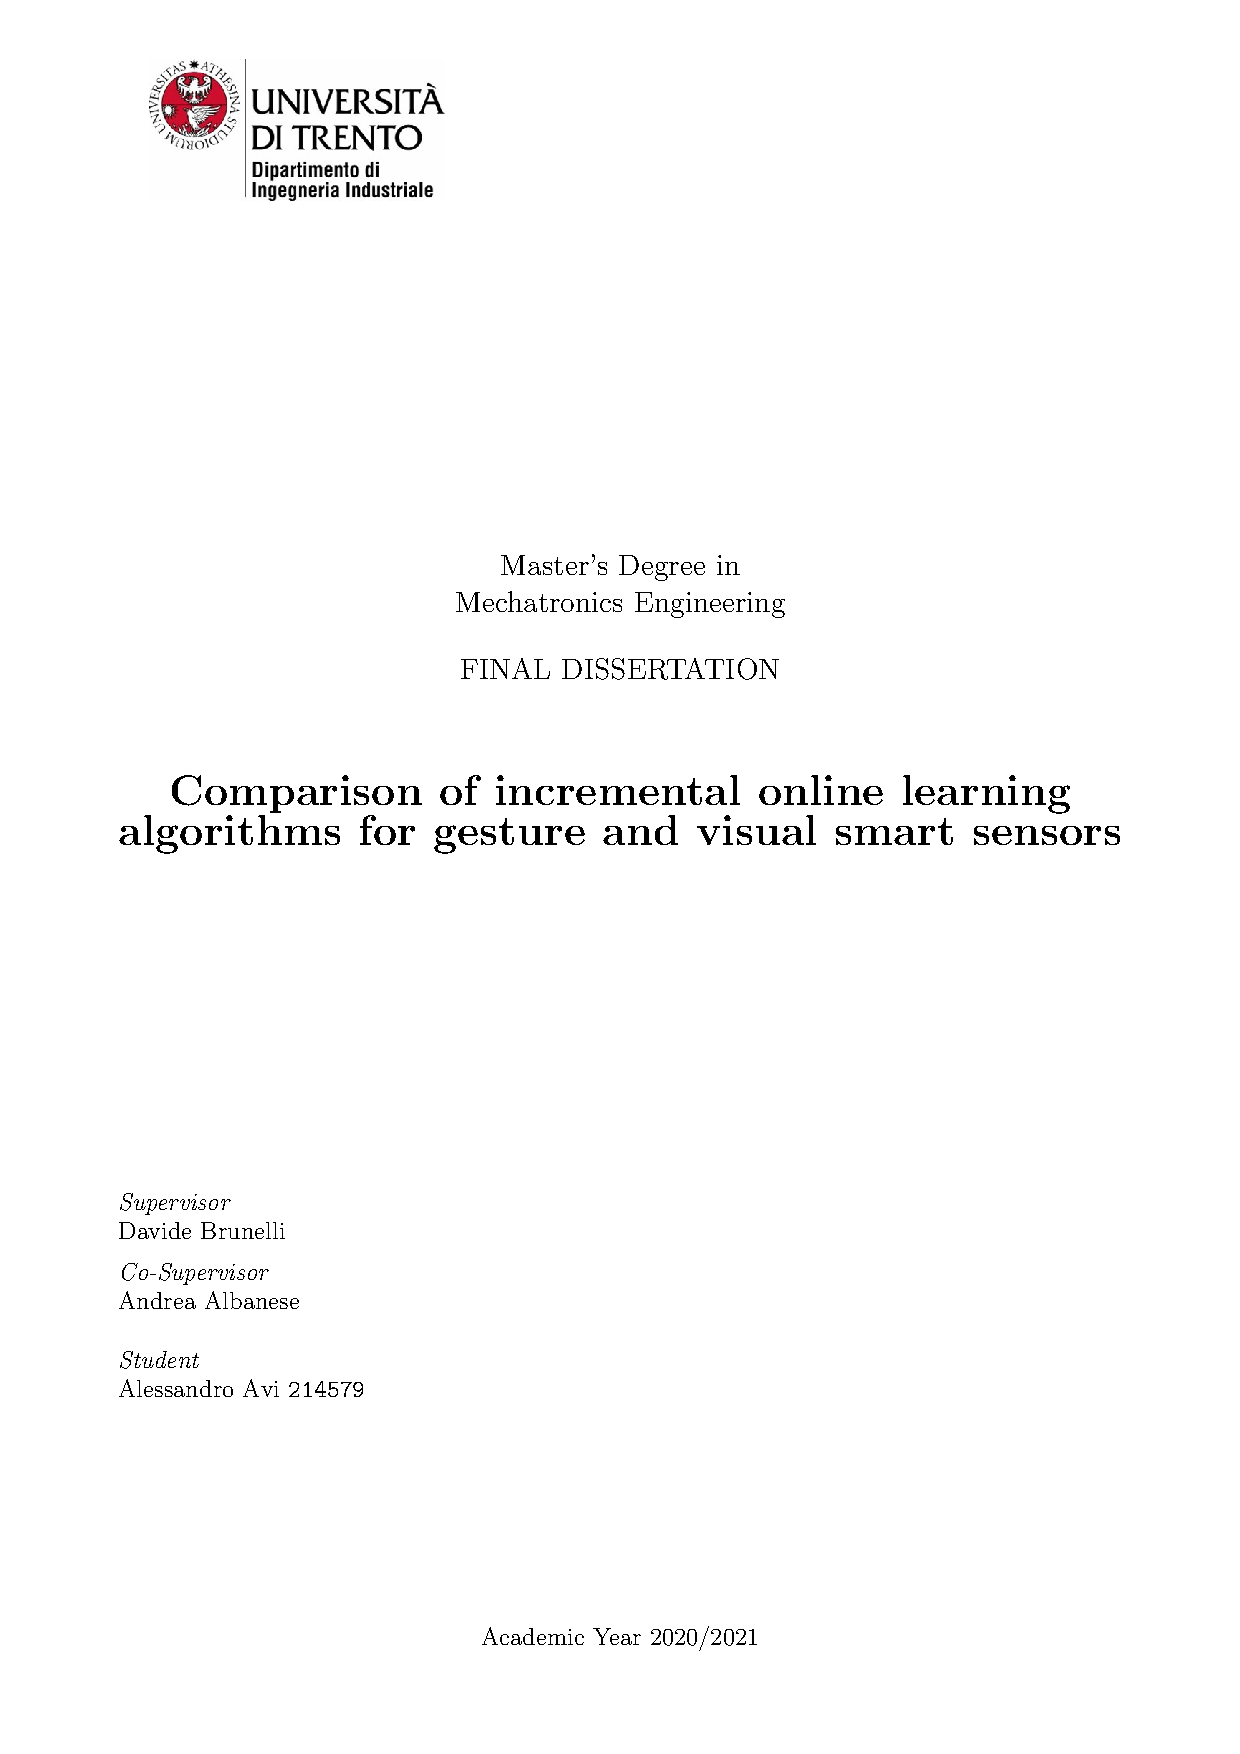
\includepdf[pages=-]{Figures/frontespizio.pdf}
\end{figure}

\afterpage{\blankpage}

\chapter*{}
\vspace*{\fill}
\textit{"Frase"} 
\begin{flushright}
Mario Rossi
\end{flushright}
\vspace*{\fill}

\afterpage{\blankpage}





%\afterpage{\blankpage}
\tableofcontents
%\afterpage{\blankpage}
\listoffigures
\listoftables
\afterpage{\blankpage}



%\mainmatter

\mychapter{0}{Introduction}

\pagenumbering{arabic}
\label{intro}
Machine learning (ML) applications on small devices, known as TinyML, is becoming more and more popular. The usage of this type of technology on micro controllers (MCU) is becoming more and more indispensable and helpful in several fields such as industrial applications, agricultural automation, autonomous driving, and human-machine interaction. One of the main fields in which TinyML is well suited is Internet of Things (IoT). Here, machine learning is applied on small devices and it can be exploited to revolutionize the basics of IoT networks.\\
The ability of embedded systems to perform high-level and smart data elaboration makes it possible for the IoT pipeline to change from cloud computing to edge computing. This transformation comes with great benefits and additional challenges.
First of all, the traffic on IoT networks is drastically reduced. In fact, by performing inferences and predictions directly on the edge the raw data gets compressed into smaller sequences that are dense of information, reducing the quantity of data moving in the IoT networks. This allows to diminish the energy consumption dedicated to the entire system as well as the system responsiveness and efficiency.
Edge computing lowers the traffic in IoT systems but also reduces the computational weight in cloud servers. This results in reduced times of computation and communication between edge and cloud which, if combined with the ability of the MCU to perform autonomous decision, reduces the latency of real-time applications improving the overall experience.
Moreover, IoT network privacy issues can be addressed by reducing transmitted data, and consequently reducing the possibility to have unwanted interceptions.
At last the usage of ML on small devices allows to better customize the device, and make the devices better suited for specific jobs. \\
Of course, the application of such a technology comes with a cost, which is the increased complexity and higher amount of vulnerabilities. Thus, it is necessary to set up robust systems that are able to ensure the system security (due to the high number of vulnerable nodes), and high performances, no matter the limitation of the device. It is in fact known that the main downsides of embedded systems and small MCUs are their limited hardware, small memories, and low-capacity batteries. Another important aspect concerning TinyML is the training and deployment of the model, which is typically performed on a powerful device and later loaded on the MCU using compression strategies. The main challenge is how the compression of big and well performing models is performed, especially because the model needs to maintain high accuracy with a low memory footprint. The creation of efficient and optimized compression strategies has been one of the main focus of recent research in the TinyML. \\
Another relevant challenge for the application of ML in IoT systems comes directly from the environment in which IoT smart nodes are deployed. Depending on the specific application, it is usually the case that the context in which an IoT device works is not characterized by a static behaviour. Meaning that the phenomenon to be monitored is able to change or evolve over time, thus data recorded can consequently evolve and change its main features. This can make difficult using ML models because they only perform inference and lack the ability to adapt to changing scenarios. It is clear how devices, set up in this way, are vulnerable to the context drift aforementioned.
By training ML models for a specific context and later deploying them in the real world, it is expected a drop in accuracy which can make the application itself not reliable. It is then obvious how an application of simple ML inference on such environments is not the best solution. To contrast this issue, it is necessary to implement the so called Continual Learning (CL) algorithms. CL is a machine learning approach that allows ML models to perform training in real-time and continually keep up-to-date the model weights. The implementation of this method comes with new challenges and limitations which are mainly related to memory management and strategies for the implementation of real-time training which also keep in consideration the optimization of resources.
\bigskip

Continual learning methods lead to a real-time training based on the data incoming. This allows the model to change and fine tune its weights and structure to better contrast the context drift.
An additional feature that can be easily added to CL is the ability to recognize never seen classes. This, if paired with the model's ability to extend its structure, allows to create a flexible model that is able to allocate new weights and biases for better predictions.
An important problem that tackles basic applications of CL is catastrophic forgetting. Catastrophic forgetting is a phenomenon that occurs when model trained in real-time overfits new data. This makes the knowledge related to past tasks be replaced by new knowledge, thus forgetting the initial scenario which leads to a reduction of the model performances over time. This aspect can be reduced by applying preventive mechanism inside the back propagation that control the parameters update. \\
The implementation of CL in industrial applications is not a new topic in the research world, but its implementation on tiny devices is just started to become more and more popular. One common application is CL in industrial scenarios, mainly for monitoring purposes on heavy machines.
The main contributions of this study concern the application of CL in two different applications. The objective is to understand if CL is a feasible solution for TinyML and if its use is actually effective for the generation of autonomous and self adapting models. In this study, a light framework that is easy to connect to a pre trained classification model was developed. The system substitutes the last layer and continually performs updates on weights and biases, and also extends its shape for flexible adaptation to new classes. The system is able to use different state-of-the-art strategies that are tested and compared in two experiments with the aim of understanding if it is possible to: i) maintain or improve the accuracy of the model; ii)contrast catastrophic forgetting; iii) digest and learn classes of never seen data. Both experiments concern the application of ML for the classification of data coming from different sensors. \\
The first application regards the analysis of accelerometer data. In this experiment the user holds the accelerometer sensor in its hand and records a time series of accelerations while drawing letters in the air. The idea is to apply ML to classify the data and recognize the letters written. The model created is initially trained for the recognition of the pattern that characterize the five vowels. Later CL is applied to the experiment and the model is exposed to new data representing three new consonants. The aim of the experiment is to let the ML model learn new patterns by performing a real-time training.
The experiment can be considered a simplification of a real world applications, but it is a clear example of how a CL model can behave in these scenarios. This application can be extended in a real-life scenario such as the monitoring of vibration patterns of heavy industrial machinery. \\
The second application concerns the experimentation of CL on a CNN model applied on an OpenMV camera for the visual recognition of digits from the MNIST dataset. The idea consists of initially train the model to recognize only the digits from 0 to 5 and later use the CL framework developed for applying a real-time training on the remaining digits. This second experiment can be extended to applications where a camera is used for a visual control of defects on products in a production pipeline.  \\
The work carried out in this study shows that the application of CL on tiny devices is possible. Even though the CL strategies are applied only on the last layer the results are satisfying and in both examples all the classes were correctly digested by the model. These tests show that a model equipped with a CL system is able to expand its knowledge and learn more classes, specifically 3 for the letters example and 4 for the digits example. The devices are able to maintain a reasonable accuracy at the end of the trainings that drop from the original frozen model accuracy by only 10.7\%.
The study performed is a good example that shows the capabilities of these tiny devices. It proves that machine learning applied on MCUs is a technology that has a huge potential and deserves more attention. CL can lead to smarter, more efficient, better performing systems in the IoT field and in industrial applications.
\bigskip

The Thesis is organized as follows. The first chapter contains an introduction to the theoretical aspects of Machine Learning (ML) and Continual Learning (CL). At first, basic concepts of Machine Learning are described, then the focus moves towards Continual Learning (CL) where also some state of the art papers are discussed. The chapter then describes some applications of ML on microcontrollers (MCUs) with also a brief explanation of advantages and disadvantages of cloud computing and edge computing. The second chapter briefly explains the hardware used in this study. The study uses two different hardware for two different applications. Therefore, the chapter initially describes the STM32 Nucleo MCU, and later focuses on the OpenMV camera. The chapter concludes with a short explanation of how ML can be applied on tiny devices. In chapter three the system implementation is described. Here, the steps performed for implementing CL training on MCUs are described, followed by an explanation of the basic structure of the TinyOL system. Then, all the algorithms implemented are illustrated in detail with also some considerations about memory and computational power. At last, the general idea of the two applications is demonstrated. The fourth chapter shows in detail the experimental setup. Here, itcan be found all the information needed for replicating in detail the tests. This chapter describes: i) the collection of the dataset; ii) the training and evaluation of the frozen models; iii) the detailed execution of the tests using the MCU and a laptop. Chapter five contains the results obtained from the training. At first, it provides the detail about the comparison between training performed on a laptop and training performed on an MCU. Then, the the results from all algorithms applied in the experiments of gesture recognition and image classification are explained. The results contain information about accuracy, precision, F1 score, memory used and time of inference. In the last chapter conclusions about the work done and possible future implementations are discussed.


\chapter{Related Works} \label{chap:relworks}

\section{Introduction to Machine Learning}
Machine learning is a branch of Artificial Intelligence (AI) that deals with the creation and training of models that have the ability to learn from data. This technology is a growing field of data science that is gaining popularity thanks to its flexibility to adapt to many problems. Machine learning models can be trained for different purposes such as regression of unknown systems, classification of data, predictions of data behaviour and artificial data generation.\\
An ML model is a file generated from a training procedure set up with specific characteristics. Training sessions are usually customized to make models learn tasks that can be applied in real world scenarios on data that have characteristics relevant to the training dataset. The simplest ML model, called Deep Neural Network (DNN), is composed of neurons grouped inside layers that are connected in series as displayed in Figure \ref{fig:modelstructure}. The layers can be divided in: input layers, hidden layer and output layers. 
The input layer is the first of the model. Here the input array (or matrix) is inserted and each neuron of the layer is composed of a value from the input sample. 
The output layer is the last of the model, this contains the elaborated data. Depending on the use of the model and on its characteristics the output values can represent different types of information, such as bounding boxes positions, percentages representing classification, artificial generated data,... 
The hidden layers are all the layer that can be found in between the first and the last layer. The type of hidden layer can change depending on the application and the type of elaboration that is applied on the data. The model represented in  Figure \ref{fig:modelstructure} iscomposed of only fully connected layers. This type of layer is characterized by neurons that are connected to every single node from the previous and following layers. Some examples are: convolutional layer, which are used to apply the convolution operation on images; pooling layers, which are used for extracting the most relevant features from an image while reducing its size; dropout layers, which are used for randomly nullify input values for avoiding overfitting; normalization layer, which are used for scale the input data to suitable intervals with the aim of removing bias. \\

\begin{figure}[h!]
    \centering
    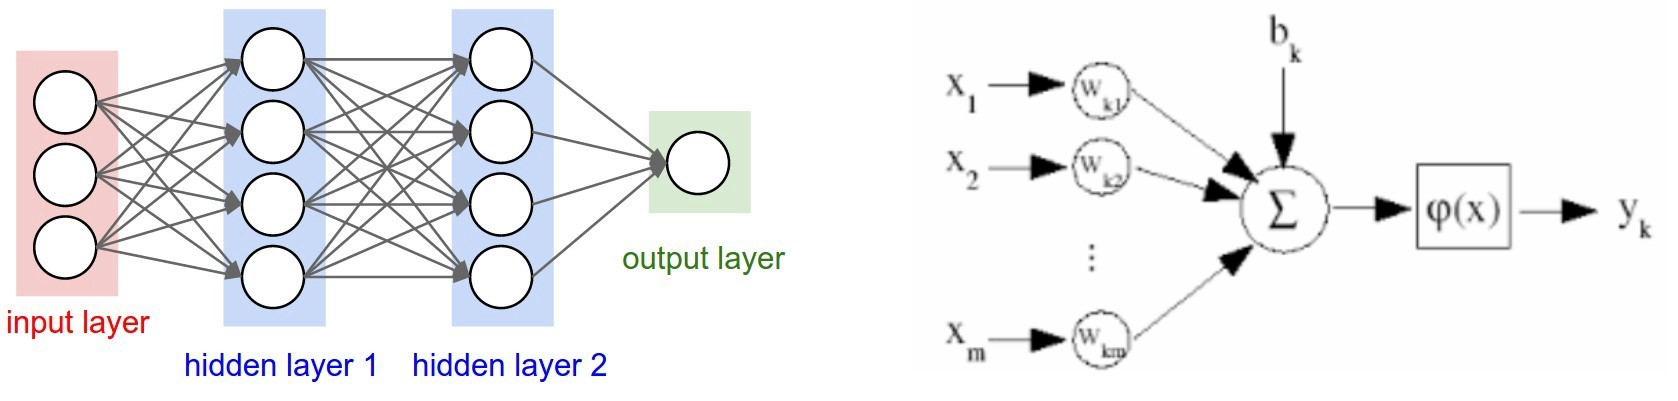
\includegraphics[width=140mm]{Figures/Chapter1/modelstructure.jpeg} 
    \caption{On the right an example of layers inside a ML model. On the left a scheme explaining how a neuron behaves. IMMAGINE NON DEFINITIVA}
    \label{fig:modelstructure}    
\end{figure}

An important role is played by the smallest element in a ML model, the neuron. This component is responsible for the evolution of the network and the learning and adaptation abilities. A neuron, or node, can be seen mathematically as a function that takes many inputs and generates one single output. Figure \ref{fig:modelstructure} shows one node that takes all the inputs, multiplies each one for a custom weight, sums them together and adds to it a biased value. Then the result of the addition is fed through an activation function which is used for introducing a non linearity in the model. The type of activation function is usually defined depending on the application of the model. Some well known functions are Softax, ReLU, Sigmoid, Linear, and Hyperbolic Tangent. 
The most common activation functions in CNN and DNN models are Softmax and ReLU. 
The Softmax activation function is specifically used in classification layers because it has the ability to convert the values of an array into values that sum up to 1. This function is particularly useful in classification applications because it can be seen as a function that maps an array of values to an array of probabilities. Where each probability is a measure of how confident the model is in assigning an input to a class. The ReLU activation function, on the other hand, is used only on the hidden layers. Its use is typically preferred to Hyperbolic Tangent or Sigmoid because it introduces less complexity in the computation of the Stochastic Gradient Descend (SGD) and avoids a problem known as Vanishing Gradient \cite{ReLU_explanation}.\\
ML trainings can be categorized in several groups depending on how the training is performed. The main groups are:

\begin{itemize}
\item Supervised learning: a type of training where the model is provided with input samples and the desired output. The model is trained to yield the same outcome as the one provided by using a feedback for correcting weights and biases. Supervised learning is commonly used in classification problems (when a model is trained to categorize data in groups) and in regression problems (when a model is trained to find the relation between variables).
\item Unsupervised learning: a type of training where the model is provided with only input data. During training the model learns patterns of data and categorizes them in groups. This is commonly used in problems where the user is unsure about the properties of the dataset.
\item Reinforcement learning: a type of training where the model is provided with input data and rewards when outcomes are correct. The goal of the model is to elaborate the input data and compute an output, depending on the rewards obtained the model learns from its mistakes and tries to maximize the reward that it receives from future steps. This type of training is commonly used for minimization problems such as industrial automation (minimization of robot paths), data processing, and chess games.
\item Transfer learning: is not a real type of training, but more a technique that is used to transfer already gathered knowledge. This method takes an already trained model and fine-tunes its last portion. The idea usually is to use state-of-the-art models that are trained for generic purposes and fine tune them to be applicable in more specific applications (use a state-of-the-art model for object identification and fine tune it to recognize humans in infra-red images)
\end{itemize}

Figure \ref{fig:supervised} shows the main characteristic of the different training types aforementioned.

\begin{figure}[h!]
    \centering
    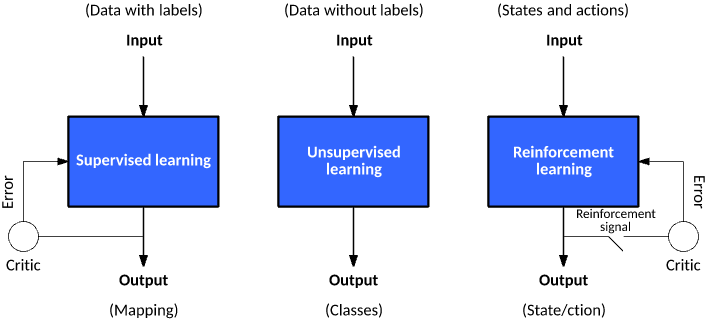
\includegraphics[width=140mm]{Figures/Chapter1/supervised.png} 
    \caption{Characteristic summary of supervised, unsupervised, and reinforcement learning.}
    \label{fig:supervised}    
\end{figure}

The training step is the process that allows a model to change its weight and make them converge toward an optimal state where the error committed by the prediction is minimized. An example of training step is the following. The model receives an input sample and propagates it through all hidden layers. Once the data reaches the output layer, a prediction is computed and later compared with the ground truth label (if the training is supervised). A loss function is used for computing the error performed by the prediction, then the back propagation algorithm is performed. This procedure consists of correcting all weights and biases of all previous layers with the aim of minimizing the error of future predictions. If the training is performed on a big enough and heterogeneous dataset, parameters should be now in a condition that allows the model to consistently make predictions that satisfying results.\\

Depending on the types of layer used inside a ML model, several model types can be defined. Different structures can be exploited for many applications, some examples of basic models are DNN, CNN and autoencoders. \\
Models that are composed of only fully connected layers, also called fully connected deep network are well suited for regression and classification of data. These layers are capable of performing elaboration of data simply by relying on the use of activation functions and correction over the weights and biases. 
Convolutional layers are well suited for the elaboration of images. They use filters that move over an image and perform the convolution operation. This is one of the basic procedure used in image processing for the extraction of features from matrices of data (like pixel values inside an image). Usually these types of layers can be found in the initial portion of a Convolutional Neural Network (CNN) model. These models are usually divided in three part. The first is composed of multiple convolutional layers used for feature extraction. This is followed by flatten layers that are used for transforming matrices in arrays. The last portion is composed of fully connected layers that elaborate and then classify the data.	\\
Other types of models are autoencoders. These models can be thought as generative models, because thei behave as constructor of lost data. An autoencoder is composed of two groups called Encoder and Decoder. The Encoder is just a sequence of fully connected layers with decreasing size, while the Decoder is a sequence of fully connected layers with increasing size. The goal of these types of models is to take an input samples, compress it into a smaller size, in what is called bottleneck, and then reconstruct the compressed array into the original values. If the training is done correctly, the Encoder can be discarded, and the Decoder part can be used as an artificial generator of data.\\
Figure \ref{fig:structures} shows some examples of ML model structures aforementioned.

\begin{figure}[h!]
    \centering
    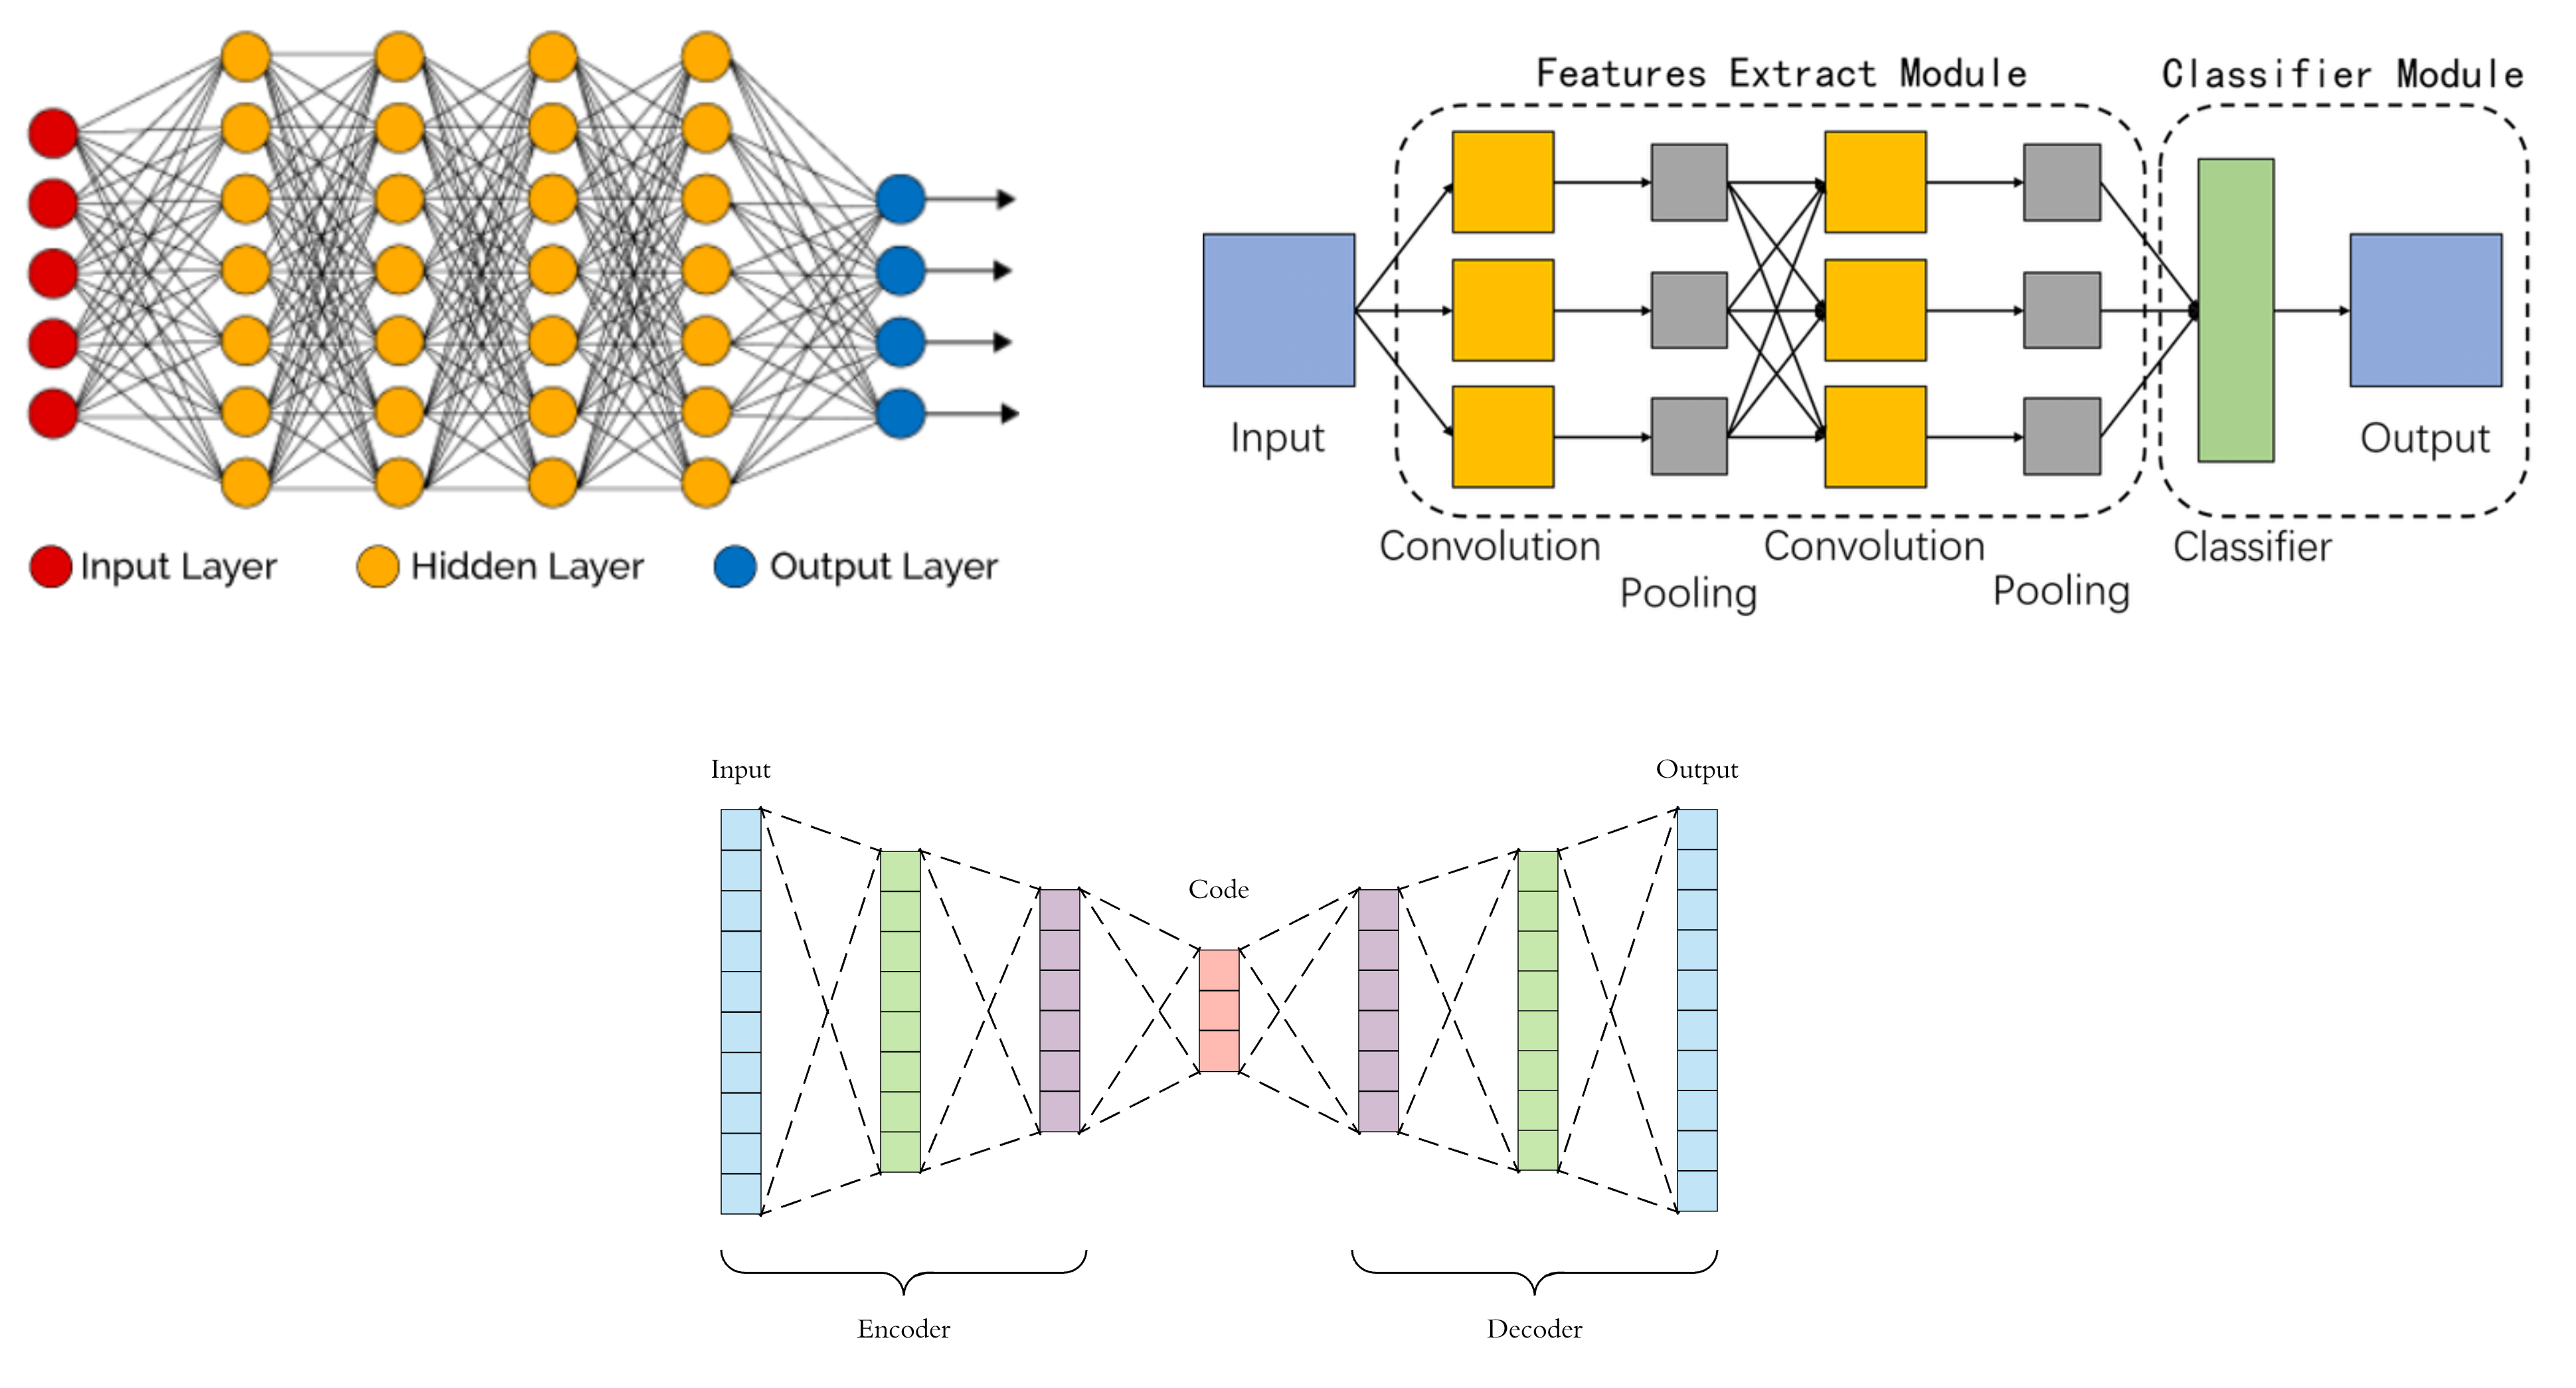
\includegraphics[width=140mm]{Figures/Chapter1/structures.png} 
    \caption{Block diagram showing an example of ML model structure: DNN, CNN and autoencoder. IMMAGINE NON DEFINITIVA}
    \label{fig:structures}    
\end{figure}  

\section{Continual on- line learning}
% introduzione a problema del ML mode, esiste CL
% spiegareo cosa è CL - OK
% spiegare uso, utilizzo, come mai serve CL, a cosa è utile - OK
% spiegare i problemi che vengono introdotti, cosa deve aggirare - OK
% iniziare a parlade di CL nella research, tipologie di algoritmi, accennare a algoritmi gia sviluppati
% apralre di altri studi relativi a CL
Applications of machine learning are based on the use of trained models for the elaboration of data. One of the main aspect regarding application of ML models is their capability to perform only inference over input data. Most times systems implemented with the only purpose of performing inference are enough for typical application purposes. But in other cases, the use of ML models capable of only predictions is not enough. These scenarios are characterized by not static environments, which are subjected to continuous evolution and changes. In such scenarios the data that is recorded and fed to ML models is subject to drifts. This means that if a model is trained on a static dataset containing data from the environment, it can quickly become obsolete. These models are not able to self-adapt to the context changes, making the accuracy, performance and reliability drop. Scenarios like these are very common in TinyML applications, mainly because tiny devices are usually deployed for extended periods of times, where the context of recorded data can change quickly. To overcome the problem of obsolete ML structures it is necessary to implement agents that make models self-adjust and autonomous. A branch of ML that specifically works on this is Continual Learning (CL). \\
The main characteristic of CL is the possibility to take a pre-trained model and update its parameter to adapt them to new data. These trainings are hard to perform on collections of samples because old data is quickly discarded and because usually there is no availability of storage (example: embedded devices memories are small). The solution is to train models in real-time on streams of sequential data that are elaborated and immediately discarded. Continual Learning focuses on the implementation of autonomous agents that control data streams and real-time ML trainings, with particular focus on the implementation of fine tuning strategies for the prevention of out of date models.\\
Continual Learning is a paradigm of Machine Learning where models are strategically trained in real-time with streams of data presented sequentially. The main characteristic of CL is the development of agents and processes that can adapt to the situation, train models and increasingly improve their complexity and performances. These aspects makes CL models very suited for applications in dynamic scenarios, where the context data is subject to drift and evolution. To improve the flexibility of CL models another feature can be added to the ML models, the ability to recognize and adapt to new classes of data. This is an easy to implement element that directly improves the complexity of the model and its autonomous behaviour. Models that are equipped with this, are able to allocate new weights and biases dedicated to the prediction of data for the specific class. Systems structured in this way require for more preliminary work and for more complex implementations, but allow for deployments that require little to no maintenance. \\
Not all CL implementations require the use of systems with the ability to recognize new classes. In some cases the sudden appearance of new tasks is not of relevance for the application. It is important then to distinguish the possible types of data streams. Paper \cite{maltoni2019continuous} proposes the following classification:\\

\begin{itemize}
\item NI: New Instances, data samples contain new patterns of already known classes (example of image application: classification is done on dogs and cats, inputs present different illumination or different background)
\item NC: New Classes, data samples contain patterns belonging to new classes. The model is not able to recognize in a different label these kind of samples. (example of image classification: classification is done of dogs and cats, inputs presents images of ducks)
\item NIC: New Instances and Classes, data samples containing both patterns of already known classes and samples regarding new classes. This is the most complete scenario and is the one that better represents real world applications.
\end{itemize}

The implementation of CL systems allows for improvements and enhancement of ML capabilities but it comes with additional problems and challenges. One of the main aspects to be aware of is catastrophic forgetting. Catastrophic forgetting \cite{french1999catastrophic} is a phenomenon that occurs when a model, trained in real-time, starts to drift from the original context, making the model forget the original knowledge in spite of new tasks. This problem is directly correlated to the real-time training procedure that tries to minimize the loss function at every step with no constraint. Usual off-line ML trainings compute the back propagations on entire batches of data. This makes the correction on the parameters be dependent from a group of samples, which makes the ML model learn to optimize the classification of all data inside the batch. On the other hand, a real-time training updates the weight and biases only with information coming from the last sample. If no control is applied on the update, the model can easily and quickly overfit data samples, making the model drift from its original state which would make it forget the original knowledge. It is then of extreme importance to develop strategies that are able to maintain control over this aspect. In today's research many algorithms have been developed with the aim of performing CL with a look over catastrophic forgetting. Paper \cite{maltoni2019continuous} contains a good classification of the main types of strategies that can be adopted. Additionally summary \cite{lesort2020continual} reviews some of the most relevant and best performing algorithms. \\

\begin{itemize}
\item Architectural: these algorithms are based on the manipulation and use of particular model structures. These algorithms can be divided in explicit architectures modification and implicit architecture modifications. In the first group there are all the strategies that dynamically change their architecture and structures by cloning, adding or saving parts of the model. Examples of this groups are strategies that use dynamic allocation of new layers (like in PNN \cite{rusu2016progressive}) or dual-memories-models. The second group, on the other hand, comprises methods that contrast forgetting without modifying the structure. This can be achieved by disabling some layers with weight freezing (which blocks the ability of the model to update) or by re routing the forward pass of the model.
\item Regularization: this group contains all those approaches that base their ability to retain past memories on the use of particular loss functions. In these loss functions usually a term is added with the aim of adding control over the back propagation. This allows the model to decide which are the important memories to maintain and which are the less relevant ones. Some basic examples of these strategies are weight sparsification, dropout and early stopping.
\item Rehearsal strategies: these approaches are based on the use of raw samples from past tasks for the refreshment of old knowledge (ideally the samples that better represent the original knowledge should be used).  Note that this methods is not well suited for application on MCUs because it requires to store old data. 
\item Generative Replay: this methods implement similar strategies of the rehearsal. This time the "old" data that is given to the models is not coming from a stored samples, but it's actually data artificially generate by the model. Again these methods are not well suited for MCUs because thei require more computations and complex structures. 
\end{itemize} 

Figure \ref{fig:CLstrategies} contains a Venn Diagram showing the classification of the most used algorithms.

\begin{figure}[h!]
    \centering
    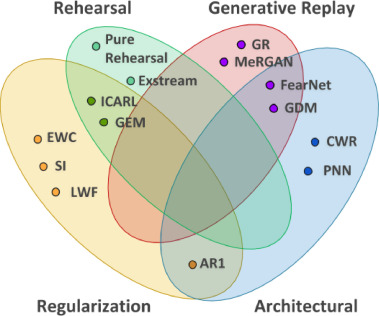
\includegraphics[width=90mm]{Figures/Chapter1/CL_algorithms.jpg} 
    \caption{Venn Diagram showing the classification of some well known CL strategies.}
    \label{fig:CLstrategies}    
\end{figure}  

As aforementioned, the Generative Replays and Rehearsal approaches are not suited for applications of MCU. On the other hand Regularization approaches are the most suited for applications on embedded systems because they require just a smart implementation of a control over back propagation. Architectural approaches can be applied on MCU if their implementation do not use big amounts of memory and many dynamic allocations. In particular, strategies classified as Implicit Architecture are easiest to implement and require the less amount of memory and computations.\\

Continual learning is an already known topic in the filed of research about machine learning. It recently stated to gain attention thanks to recent works in the field of TinyML. The applications of CL on microcontrollers and specifically on IoT devices leads to better performing systems with many benefits. Some important studies that propose applications of CL strategies on tiny devices are papers TinyTL \cite{cai2020tinytl}, Progress \& Compress \cite{schwarz2018progress}, TinyOL \cite{ren2021tinyol} and Train++ \cite{sudharsan2021train++}. All these papers propose frameworks and custom strategies applied successfully on microcontrollers for the enhancement of ML capabilities. 
Studies \cite{park2020convolutional} and \cite{disabato2020incremental} propose the use of CL on applications similar to the one used in this thesis, image recognition. The two papers apply developmental memories and k-nearest neighbour for successfully contrasting catastrophic forgetting. \\
Another important paper about CL , this time not applied on MCUs, is the the study \cite{maltoni2019continuous}. Here the author's goal is to implement several algorithms and test them to evaluate their abilities to overcome catastrophic forgetting. The study applies already known strategy like LWF \cite{li2017learning}, SI \cite{zenke2017continual} and EWC \cite{kirkpatrick2017overcoming}. Additionally the paper presents the implementation of other two custom made algorithms called CWR+ and AR1. Note that CWR+ is an improvement of an already proposed approach developed in paper \cite{lomonaco2017core50} written by the same authors. \\
An interesting application of CL strategies is proposed in paper \cite{grau2021device}. A system composed of 2 microcontrollers and a central server is used for performing federated training. The idea is to perform training on the edge and frequently merge the models on the server. This allows for applications of CL in a distributed way (useful for IoT), where devices are used for performing fine tuning over different input streams, thus allowing the merged ML model to be composed of models trained on the same application but coming from different contexts.
Another interesting study, not directly related to algorithms, is the one described in \cite{sudharsan2021imbal}. Here the authors developed an easy to attach system, called Imbal-OL, that aims at balancing real-time streams of data. From their point of view, real-life applications of CL strategies for IoT devices are characterized by unbalanced streams of data. This affects real-time trainings because models can easily overfit the inputs, thus leading to models with poor performances. The authors propose a small plug-in to be attached in between the raw input stream and the CL model that is able to apply pre-processing on the data and make the input stream balanced. \\
One of the most relevant works for this thesis is the paper \cite{ren2021tinyol}. Here the authors developed a small framework for an Arduino microcontroller that is able to apply continual learning (or on-line learning) strategies on an ML model. The systems uses an autoencoder model for the recognition of vibration patterns from a PC fan. The Arduino is mounted directly on the fan and measures the data with an accelerometer sensor. The CL system, called TinyOL, is attached to the autoencoder's last layer and it is used for recognizing the appearance of new classes and fine tuning the classification layer. The system applies one CL strategy which follows the basic principles of a standard ML training, but applied in real-time on one sample at a time. 

\section{Machine Learning on MCU}
% applicazione ml su mcu, risorse limitate, molto importante power comsumption, design del mcu, paralre di possibili applicazioni, paraldre del fatto che si fa solo inference
% parlare del rpuning, binarization, compression del meodello, state of teh art compression MCUNET
TinyML is a fast growing research area that aims at applying ML on limited devices like micro controllers. This technology has found a rapid grow in last years especially thanks to the potential demonstrated by applications in several fields such as industrial application, agricultural automation, human-computer interactions, autonomous driving. The use of TinyML allows to introduce the concept of edge computing, where computations are brought closer to the origin of the data, where devices until now were used only as collectors and transmitters of data. Edge computing brings to lots of advantages like low-latency , better privacy, security and reliability to the network end-user. It allows to move the computations from the cloud to the device itself, which brings to higher throughput and improved responsiveness in applications. Speaking about responsiveness, which is a huge deal for real-time applications, edge computing permits to decrease the network traffic. This feature comes from the fact that the use of machine learning directly on the device allows to lift a big portion of computation weight given to the central server, thus reducing the amount of data that has to be exchanged on the network, which is also compressed in size and dense in information. \\
One of the main fields in which TinyML is particularly fit and can be exploited with all its potential is Internet of Things IoT. Here the application of edge computing brings to lots of advantages already described before. Of course the implementation of such systems comes with a cost, which in this case is related to the increased complexity on which the MCU works and its limited resources. Machine learning is a field of computer science that is known to be energy and resource demanding. Using such a technology on these tiny devices is a real challenge which already has seen interesting applications and improvements in the research world. The main characteristic of MCU is for sure their limited dimensions and power consumption. This is usually a nice feature that allows to develop small systems that can live for very long period of times in harsh environments without the need of maintenance. 
Lot of focus has also given to the implementation of energy harvesting systems that, not only use very low quantities of energy but also are able to extract energy from the environment in which they live. Limited dimensions has also drawbacks, which are limited memories and limited computational power, all features that do not really match with the application of machine learning. 
In the last decade (??) the research around TinyML revolved around the implementation of efficient framework from both point of view of memory use and power consumption. Some well known systems for deployment of ML models on tiny devices developed by big companies are Tensorflow Lite \ref{}, STM32 CUBE AI \ref{}, PyTorch mobile \ref{}. All these frameworks are used for training a model on a powerful system and later load a compressed version of the model on the MCU. The main concerns is the compression of the model in such a way that it doesn't drop in accuracy even with reduced weights or quatnized values. The second aspect that concerns the use of these tools is the inferenfce performed on the device. Being that ML is a computationally heavy procedure it's necessary to be able to optimize it. Stydyes such as \cite{} and \cite{} focused on theis specific characteristic. Their main goals was to develop frameworls for the efficient application of machine learning inference.






The main challenge of TinyML is for sure the successful application of ML on such resource constrained systems. These are in fact designed to be deployed in difficult to reach places and for running for very long times. This implies that the devices should be battery power or equipped with energy harvesting hardware and their power consumption should be limited and optimized. Other limitations concern the limited computational power, which is directly connected to the CPU frequency and the battery management and the available memory. The latter is a very important topic for TinyML. It's in fact known that the application of ML on any type of device requires the usage of great amounts of memory, it's then a big challenge to be able to deploy these systems with very limited memories.\\
The application of ML on MCUs, mobile devices or in general on the edge of IoT systems it's a great advantage that can bring to some improvmenets. The key advantages are:
\begin{itemize}
\item privacy: by having the data directly processed on the node there is no change of violating the privacy policies since the possibility of interception is totally nulled
\item latency: by elaborating data directly on the edge the work load of processing that should be performed by the cloud is limited and so is the transmission of the data itself. This brings to limited time delays and allows the device to perform decisions in real-time, improving the performances of real-time applications.
\item energy efficiency: the transmission of huge quantities of data from the edge to the cloud takes a big portion of the energy consumption of an IoT system. Even if the application of NN is energy intensive it is an order of magnitude less, thus an improvement.
\end{itemize}

\subsection{Pruning and quantization}
When deploying ML models on constrained device there are two main concerns: the available memory and the available computational power. To overcome these two limitations, different techniques have been developed. Pruning and quantization are pre processing methods that can be employed on already trained models to reduce their memory footprint and their computational weight. Direct benefits of these strategies are lower power consumption, lower memory bandwidth, less storage required, all with the same performance. \\
Pruning is a strategy that is adopted after the model training. A training with good performances is required because, at each step of a pruning procedure, the model of interest is degraded and so is its performance. In most cases, the model developed for the application is bigger than actually required. This is due to the initial definition of a general structure and the following training that fine-tunes all parameters inside the model. The pruning method relies on the fact that in a ML model some parameters are redundant, not relevant or useless for the application. In fact, the strategy consists of completely removing connections between neurons that are less important for the application. The goal is to reduce the memory required by the model and the amount of computations for an inference. 
A pruning step is composed of the following actions:

\begin{itemize}
\item Evaluate the importance of each weight based on their influence on the network output and performance
\item Prune the less important weights (bring to 0 their value)
\item Re train the model that inevitably lost performance
\item Check if the memory reduction induced is enough, if not perform another pruning step
\end{itemize} 

Figure \ref{fig:pruning} contains a block diagram showing the basic steps of a pruning procedure followed by a quantization procedure.\\
An additional improvement brought by pruning is the reduced amount of computations. If done strategically, a pruning process can introduce sparsity (a localized population of zero values) in weight and bias matrices. If the sparsity is injected with a smart structure, it is then possible to reduce the amount of computations, thus improving the efficiency of inference in terms of time, energy and complexity.\\

\begin{figure}[h!]
    \centering
    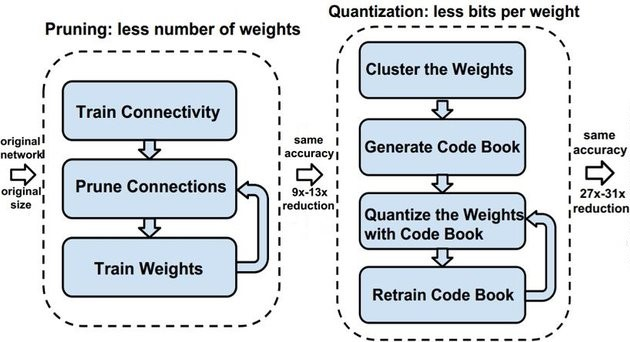
\includegraphics[width=110mm]{Figures/Chapter1/pruning.jpg} 
    \caption{Block diagram showing the steps of a pruning and quantization procedure.}
    \label{fig:pruning}    
\end{figure}  

Another method that is often used for compressing ML models is quantization. Quantization is a process that aims at reducing the $bits$ $per$ $weight$ metric. The process can be of two types: post-training quantization or training aware quantization \cite{pruning_article}. These two procedures both aim at reducing the amount of memory dedicated to each parameter, but the process for doing so is quite different. The post-training quantization consists of a rounding or type conversion of weights and biases. Common strategies rely on the conversion of the values from $floating$ $point$ 32 to $integer$ 8, which leads to a compression ratio of $\times 4$. Quantization aware training is more complex and requires the implementation of quantization strategies that are performed while training. This procedure usually reaches better results but with the added complexity of using a different training procedure. For typical MCU applications, the simple use of post training quantization yields acceptable results both in terms of compression and small accuracy drop. \\
The implementation of such procedure is quite immediate by using libraries such as Tensorflow \cite{tensorflow_quantization} which allows to perform the entire procedure with just a couple of code lines.



\subsection{Cloud vs edge inference}
Continual learning is a type of machine learning that is able to overcome context drift. This is an aspect that often characterizes scenarios where TinyML is used. By having devices and models that are deployed for indefinite times in particular places, it is to be expected that the environment in which they lye is subjected to a natural and continuous evolution. This makes the use of CL a great solution that allows models to be self adjusting to these changes and self adapting to new tasks. By using CL strategies in TinyML it is possible to reduce the maintainance to the devices that would be required because of drop in accuracy. 




\chapter{Hardware} 
\label{hardware}
In this chapter, the hardware used to carry out the experiments is described. The application of ML on MCU does not require specific types of hardware, but it requires devices that are capable of sustaining those kinds of computations. In today's market, lots of off-the-shelf MCUs are already equipped with hardware components that make the device suitable for the job. These microcontrollers only need to be correctly equipped with framework and tools that optimize ML computations. In this study, for both applications, devices based on STM microcontrollers were used. The gesture recognition application uses an STM32 Nucleo F401-RE \cite{nucleo_datasheet}, a well performing and easy to use development board. The image classification application uses an OpenMV camera \cite{openmv_datasheet}, a device equipped with a camera sensor that features an STM32 H7 MCU and is programmable in MicroPython. Figure \ref{fig:hardware_all} shows both devices: on the left the Nucleo F401-RE, and on the right the OpenMV camera. The reasons that brought to the selection of these two MCUs depends mainly on the quick availability for the Nucleo development board and the uniqueness of characteristics for the OpenMV camera.

\begin{figure}[h!]
    \centering
    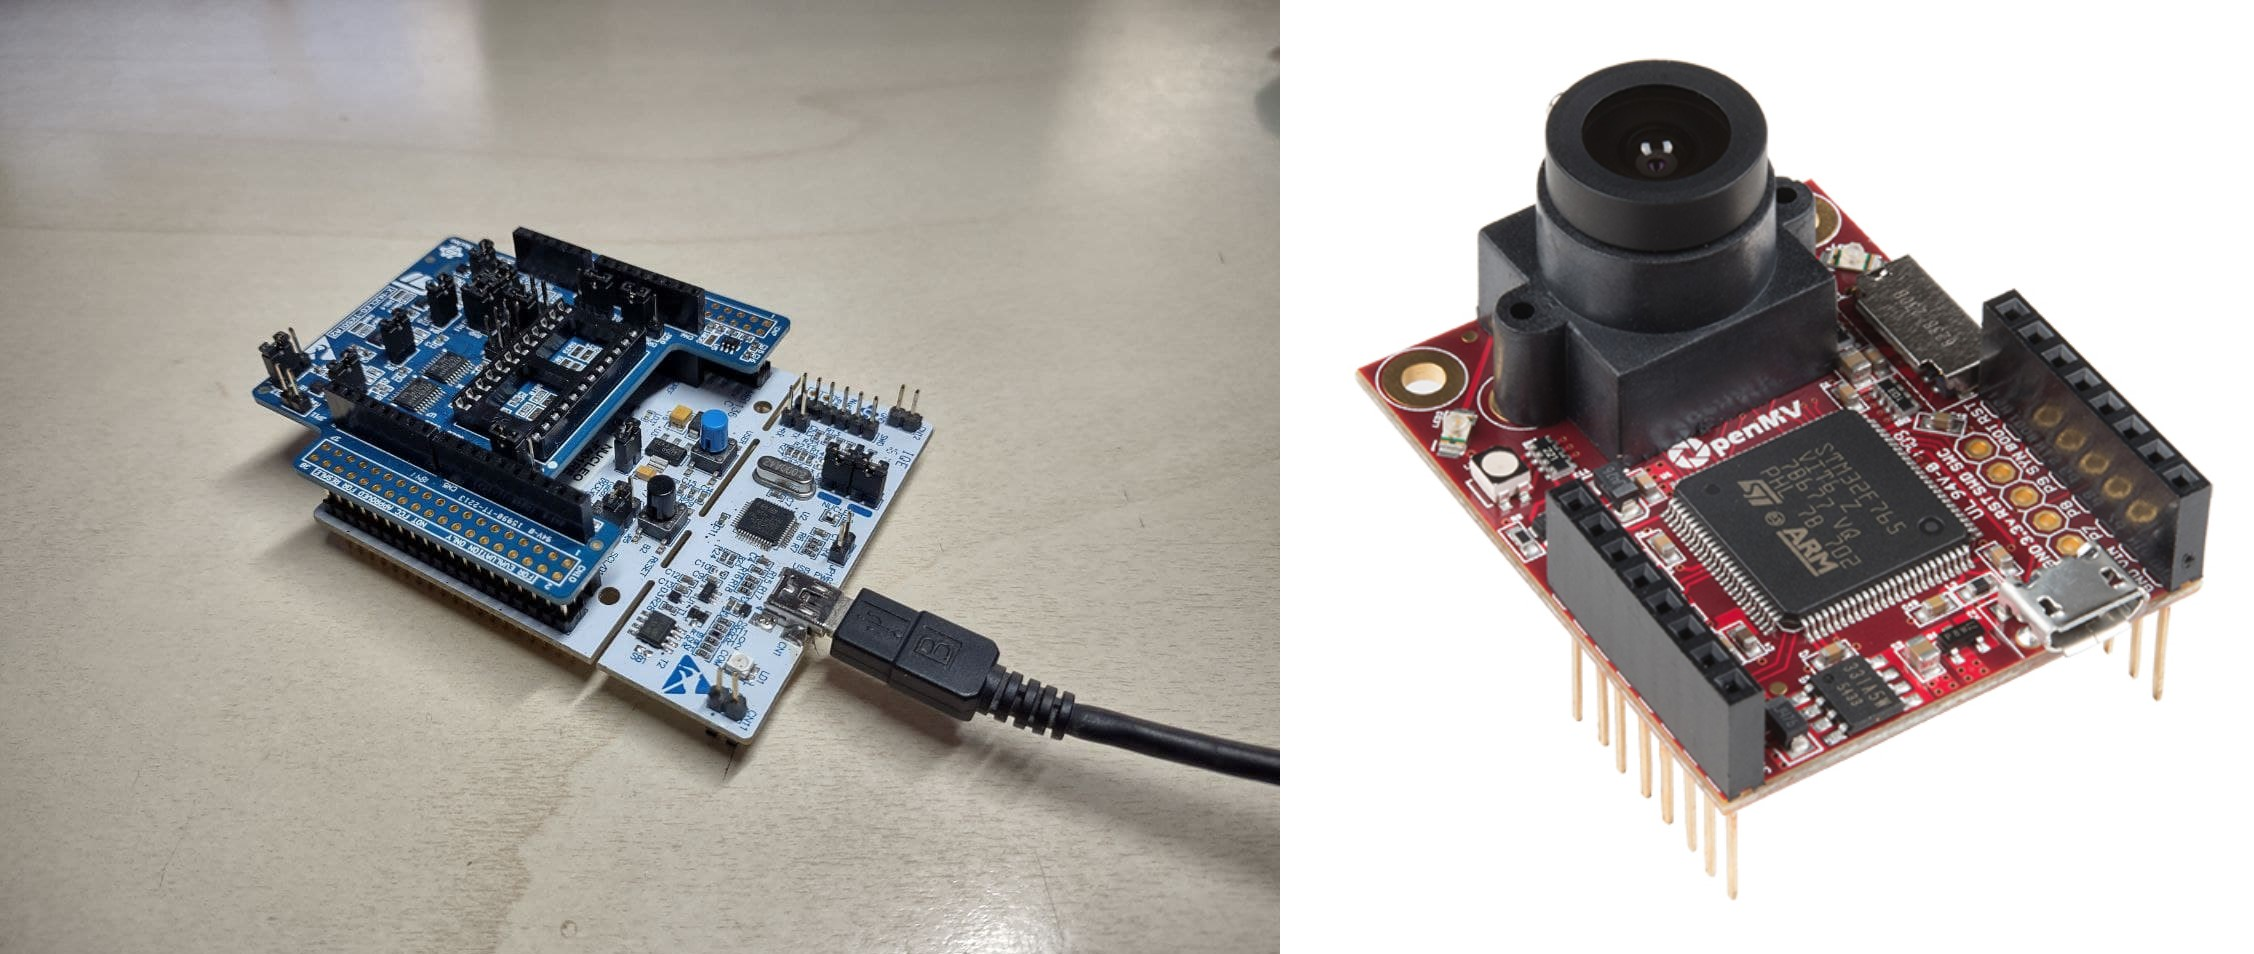
\includegraphics[width=120mm]{Figures/Chapter2/hardware.jpg} 
    \caption{Hardware used for the CL applications. On the left Nucelo ST32 F401-RE, on the left OpenMV camera.}
    \label{fig:hardware_all}    
\end{figure}

\section{Gesture recognition hardware}
The gesture recognition experiment is carried out with a Nucleo STM32 F401-RE. This device is a 64 bit microcontroller produced by STMicroelectronics that belongs to the $high-performance$ product line. This product is thought to be a flexible and easy to use development board for fast prototyping, which is also compatible with Arduino Uno shields (the internal GPIOs pin scheme is the same as Arduino Uno). Differently from other devices produced by STMicroelectronics, this MCU does not require the additional debugger/programmer ST-LINK. This component is included in the first part of the device, separated from the rest with visible gaps in the board. The Nucleo can be easily programmed in C or C++ with the the libraries and tools available in the STM32Cube package. This is a powerful software that can be exploited to perform an initial setup of any STM device, such as the definition of all peripherals and basic microcontroller parameters. The STM32Cube package also includes libraries for any device produced by STM. Moreover, using STM32Cube, the Nucleo board STM32 F401-RE fully supports the machine learning extension, namely STM-CUBE-AI \cite{stm_cube_ai}. This toolkit can be used for compressing and loading ML models on the device and later perform optimized and efficient inference in real-time. \\
The main features of the Nucleo development board are summarized in Table \ref{table:specifications_stm}.\\

\begin{table}[]
\caption{Nucleo STM F401-RE specifications}
\centering
\begin{tabular}{|l|c|}
\hline
Processor           & \begin{tabular}[c]{@{}c@{}}ARM 32-bit Cortex-M4 CPU\\ 84 MHz\end{tabular}                 \\ \hline
Memory              & \begin{tabular}[c]{@{}c@{}}SRAM: 96 kB\\ \\ Flash: 512 kB\end{tabular}                    \\ \hline
Phisical attributes & \begin{tabular}[c]{@{}c@{}}Weight: ??g\\ Length, Width, Height: ??x??x3??mm\end{tabular}  \\ \hline
Peripherals         & \begin{tabular}[c]{@{}c@{}}50 GPIOs, SPI, UART, I2C, DAC/ADC,\\ PWM, Timers,\end{tabular} \\ \hline
\end{tabular}
\label{table:specifications_stm}
\end{table}

The gesture recognition application uses ML algorithms for the analysis of time series data. The time series array contains the values recorded from an accelerometer sensor while an user is moving that sensor to write letters in the air. To acquire that kind of data, the Nucleo needs to be equipped with an accelerometer sensor shield. For doing that, it was decided to use the Nucleo shield IKS01A2 \cite{shield_web_page}, a device that can be mounted easily on the board simply by aligning the GPIO pins. The shield is equipped with a 3D accelerometer, a pressure sensor, a capacitive digital humidity, and temperature sensor. The device communicates with the Nucleo through I2C protocol and is fully supported by the libraries available on STMCube, which make its use quick and easy. Figure \ref{fig:hardware_stm} shows the two devices separately on the left and mounted on the right.\\

\begin{figure}[h!]
    \centering
    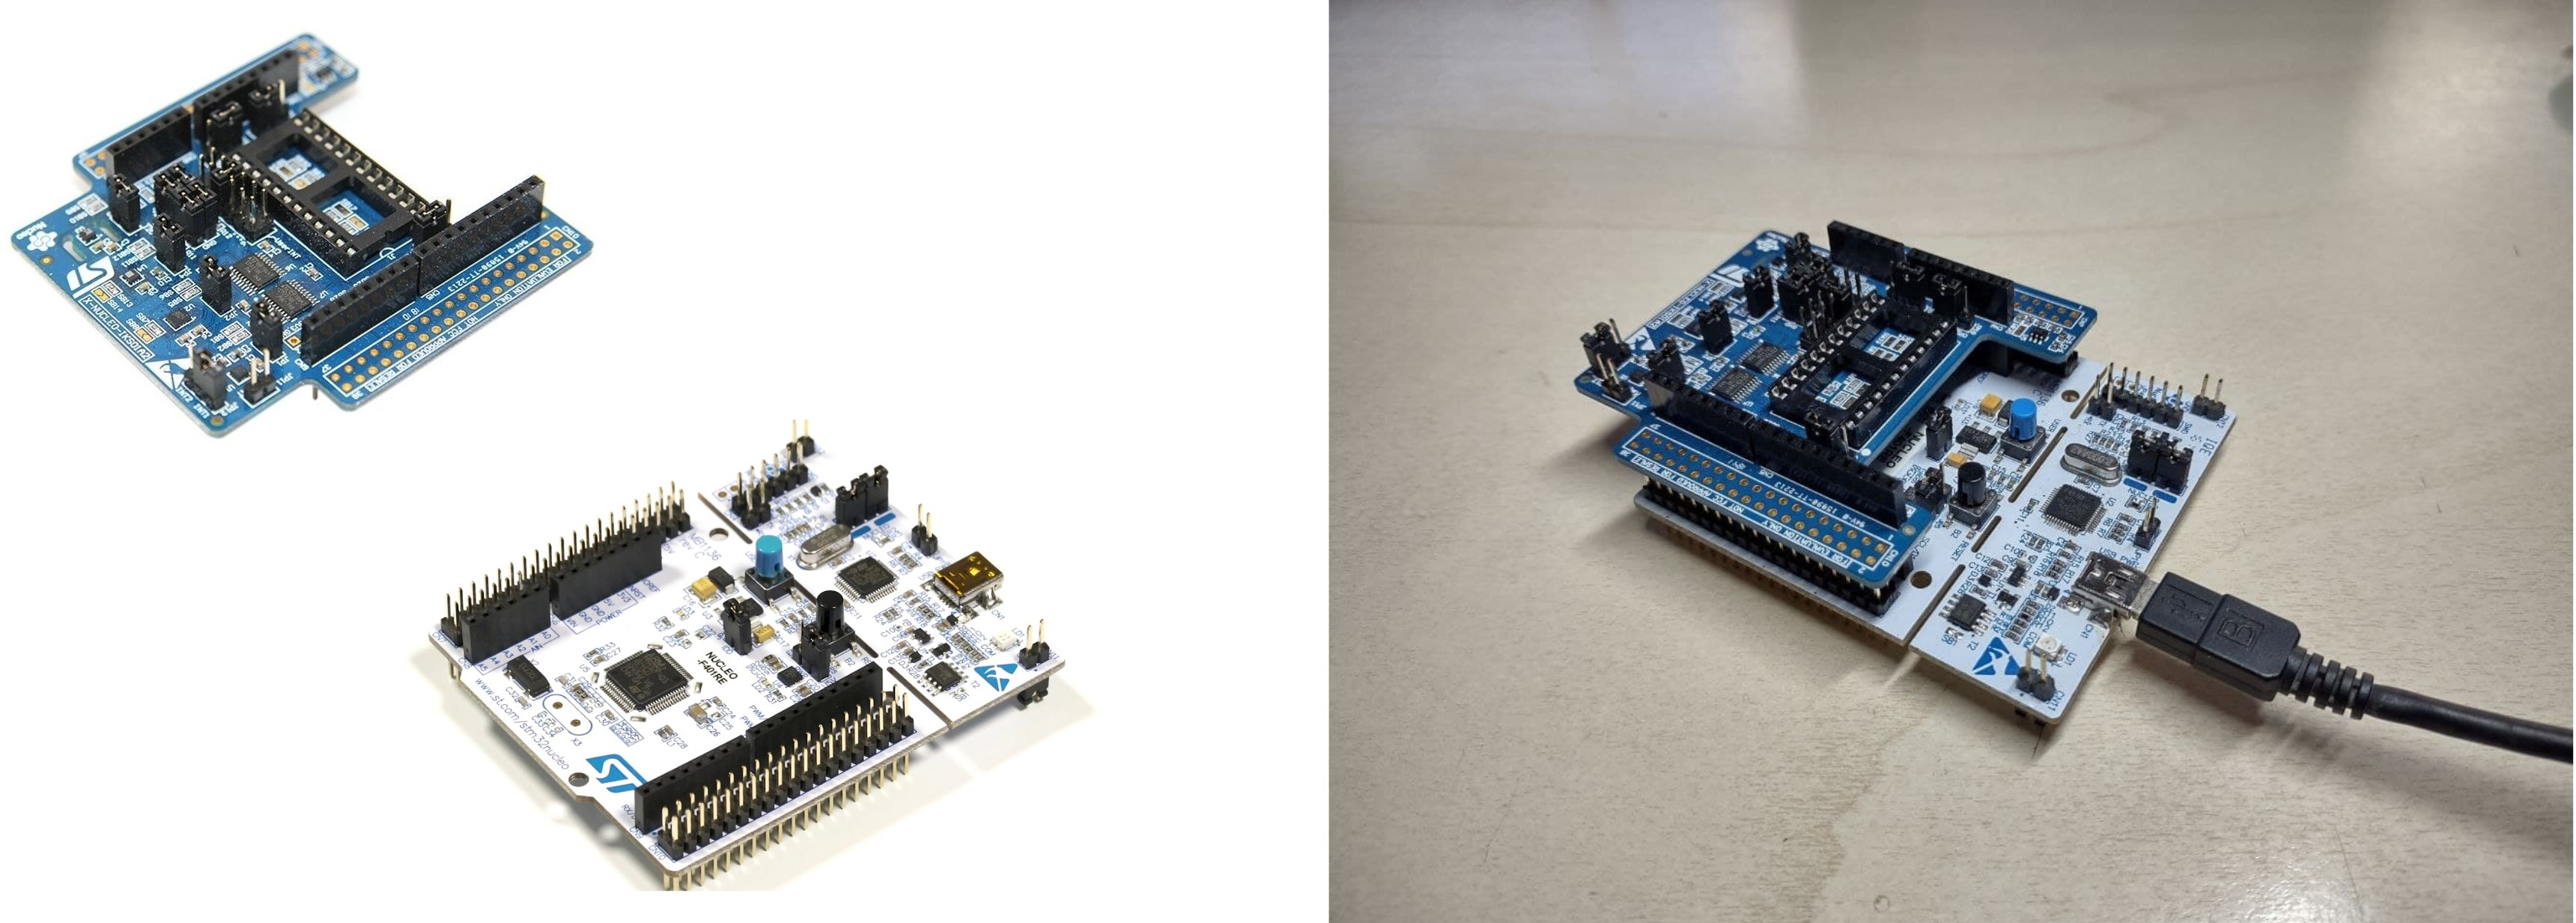
\includegraphics[width=120mm]{Figures/Chapter2/hardware_stm.jpg} 
    \caption{Hardware used in the gesture recognition application. On the left the sensor shield IKS01A2, on the right the sensor shield mounted on the Nucleo STM32 F401-RE.}
    \label{fig:hardware_stm}    
\end{figure}



\section{Image classification hardware}
For the image classification experiment, an OpenMV cam H7 plus \cite{abdelkader2017openmv} \cite{openmv_web_page} is used. This device is an affordable and expandable small board equipped with an STM MCU and a camera sensor with interchangeable lens. The OpenMV camera started as a project \cite{openmv_project} back in 2013 due to a lack of affordable, small, powerful and easy to use breakout board with cameras. Then, the idea has developed into a kickstarter that gained popularity until reaching what is today, an established product that aims at becoming the standard device for machine vision applications. \\
The device mounts the camera sensor OV5640 and an STM32 H7 MCU and it can be programmed easily with MicroPython through the dedicated OpenMV IDE. The board is equipped with 16 GPIOs which permit the camera to interact with external devices such as servo motors, sensors or other MCUs. The GPIOs can be exploited for controlling robots, drones, and machine learning systems. Some examples of successful applications of OpenMV cameras in robotic systems are: the design of a control system for rolling a ball \cite{zhou2019design} and the design of a tracking system \cite{wei2020design}.\\
Moreover, the camera comes with the possibility to mount different lenses, sensors and additional modular components. From the official website a complete list is available, some examples are: IR lenses and sensors, telephoto lens, super telephoto lens, ultra wide lens, WI-fi shield, LCD shield, and motor shield.
The possibility to add these different components or modification make the device a very well suited solution for many problems, application, and especially prototyping .\\
Table \ref{table:specifications_openmv} summarizes the device specifications.\\

\begin{table}[]
\caption{OpenMV H7+ specifications}
\centering	
\begin{tabular}{|l|c|}
\hline
Processor           & \begin{tabular}[c]{@{}c@{}}ARM 32-bit Cortex-M7 CPU\\ w/ Double Precision FPU 480 MHz (1027 DMIPS)\end{tabular}                               \\ \hline
Memory              & \begin{tabular}[c]{@{}c@{}}SDRAM: 32 MBs\\ SRAM: 1 MB\\ Flash: ext 32 MB, int 2 MB\\ Expandable with SD cart\end{tabular}                     \\ \hline
Resolution          & \begin{tabular}[c]{@{}c@{}}Grayscale: 640x480 max\\ RGB565: 320x240 max\\ Grayscale JPEG: 640x640 max\\ RGB565 JPEG: 640x480 max\end{tabular} \\ \hline
Phisical attributes & \begin{tabular}[c]{@{}c@{}}Weight: 19g\\ Length, Width, Height: 45x36x30 mm\end{tabular}                                                      \\ \hline
Lens                & \begin{tabular}[c]{@{}c@{}}Focal length: 2.8mm\\ Aperture: F2.0\\ Format: 1/3"\\ HFOV: 70.8°, VFOV:55.6°\end{tabular}                         \\ \hline
Peripherals         & \begin{tabular}[c]{@{}c@{}}GPIOs, interrupts, SPI, UART, I2C, DAC/ADC,\\ PWM, LEDs, removable camera module\end{tabular}                      \\ \hline
\end{tabular}
\label{table:specifications_openmv}
\end{table}

Because the application of this study requires a camera pointing to a screen, a small 3D printed support was created. An already available project from Thingiverse \cite{tripod_link} was modified to make the mounting of the OpenMV camera possible. The $stl$ files can be found in the GitHub repository of this project \cite{github_repo}. Figure \ref{fig:hardware_openmv} shows the OpenMV mounted on the 3D printed tripod while pointing to the computer screen during a CL session.\\

\begin{figure}[h!]
    \centering
    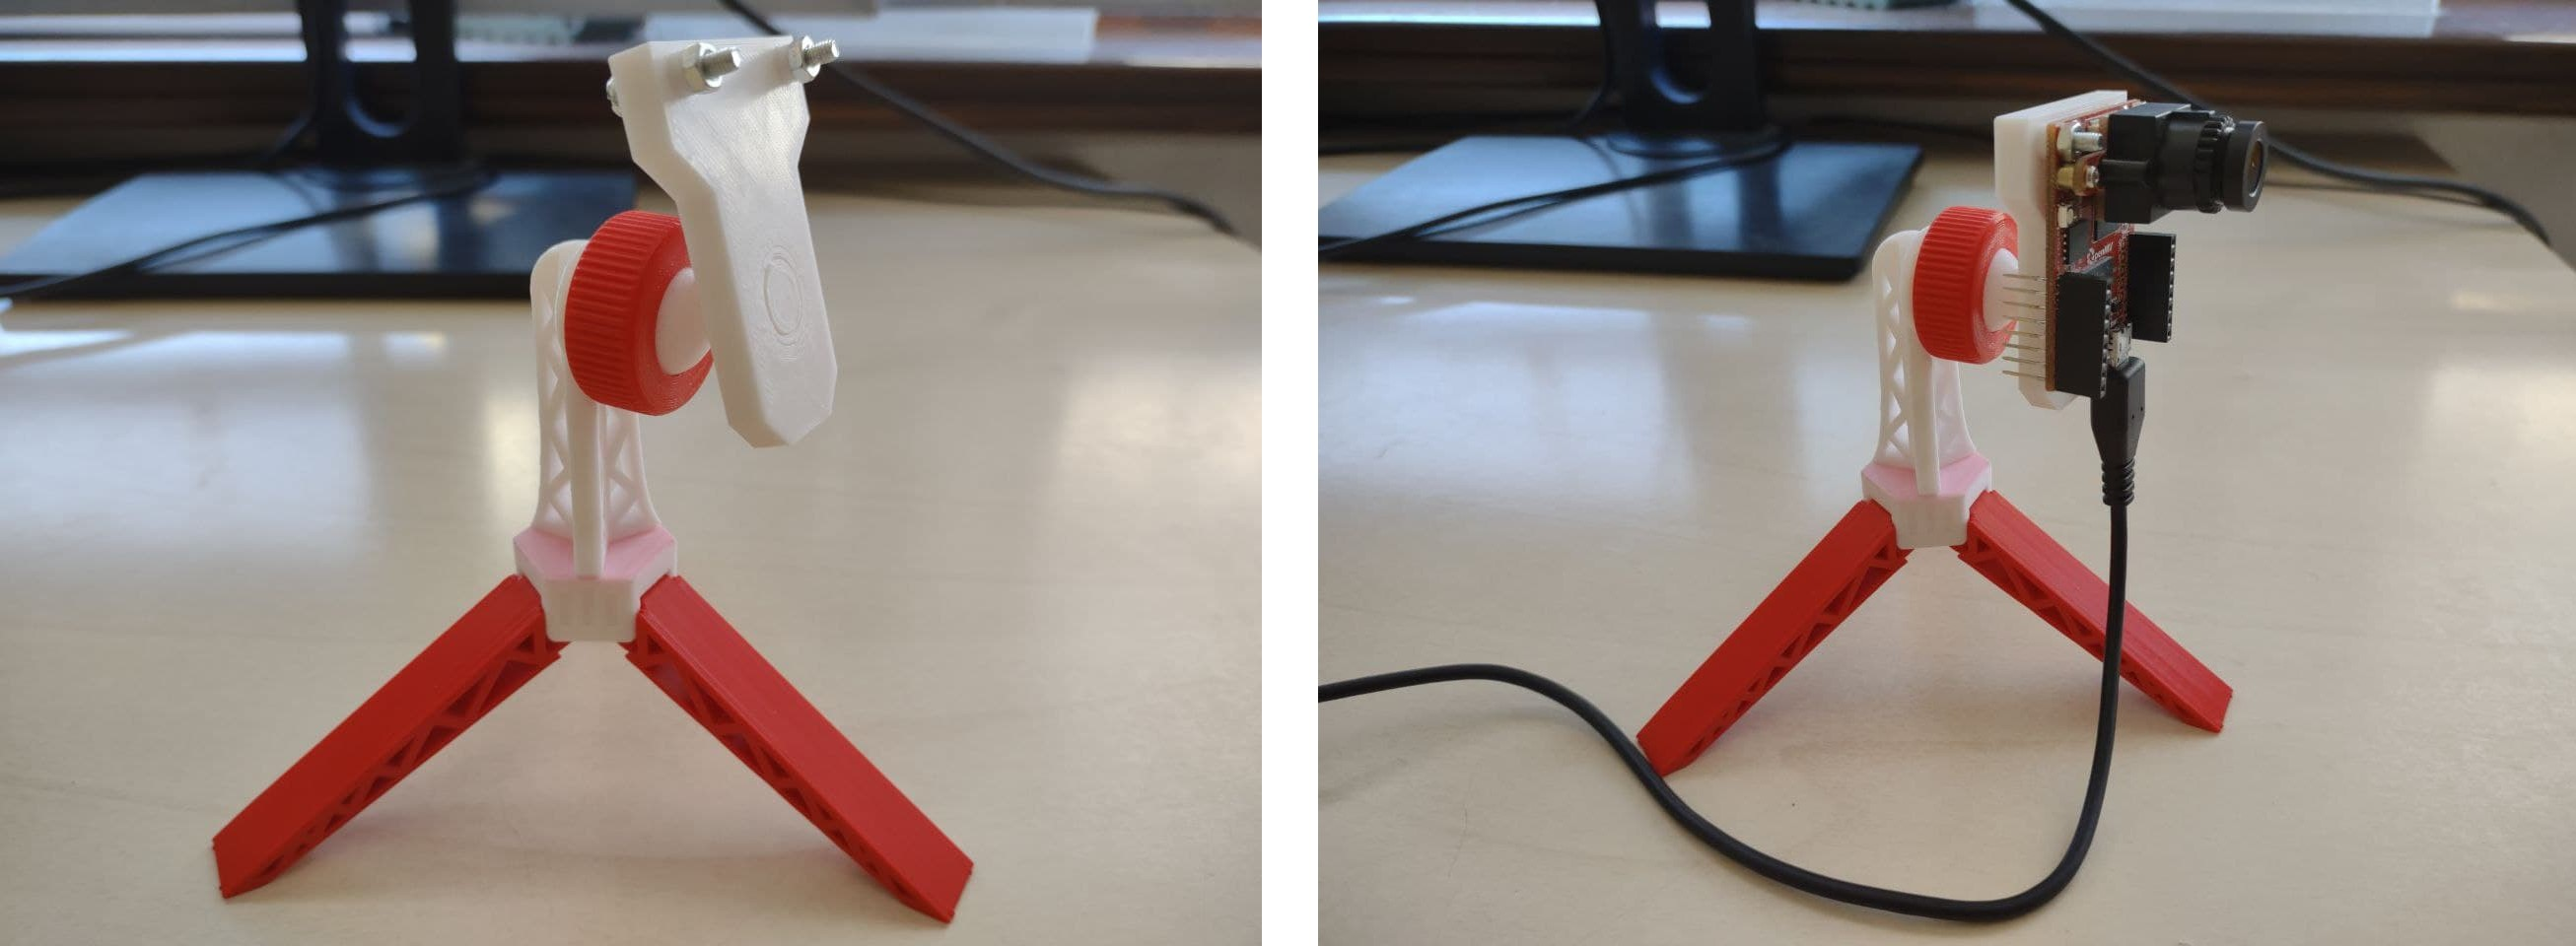
\includegraphics[width=120mm]{Figures/Chapter2/hardware_openmv.jpg} 
    \caption{Hardware used in the image classification application. On the left the 3D printed tripod, on the right the OpenMV camera mounted on the 3D printed tripod.}
    \label{fig:hardware_openmv}    
\end{figure}

\section{Machine learning support}
In this study applications it is requires to apply machine learning on the MCUs. Even if both examples use microcontrollers developed by ST, the procedure for implementing ML capabilities is not the same. \\
For the Nucleo application it is required to use ST-CUBE-AI \cite{stm_cube_ai}, an extension pack developed and supported by ST itself. This toolkit can be added quite easily from the CubeMX, a software developed by ST that helps with automatic generation of chunks of code. In this case the addition of the AI pack allows the user to not be bothered by the generation of routines and other tools required for optimized machine learning inference. By using this pack it is possible to compress, load and run ML models in an easy and immediate way with just some function calls.





\chapter{System implementation}
Continual learning is the application of real-time training on a model with the aim of generating self-adjusting systems that are able to learn from incoming data streams. As already mentioned in the Introduction \ref{Intro}, continual learning can lead to many improvements if exploited correctly in IoT applications. The main feature of Continual Learning (CL) is the ability of ML models to modify weights and biases to learn from the environment and continue to be accurate and reliable for the application. The application of CL on MCUs is still a quite new idea that only gained popularity in recent years. Applications regarding CL have already been explored before, but their application on tiny devices is still new. Some relevant studies that apply CL on MCU are \cite{ren2021tinyol}, \cite{ren2021synergy} and \cite{sudharsan2021train++}. \\
In this thesis, it is developed a CL system similar to the one proposed in the TinyOL paper \cite{ren2021tinyol}. The paper proposes a light framework, to be deployed on an Arduino, that can be attached to a pre-trained model for the application of on line learning (or continual learning). The goal is to classify vibration patterns of a PC fan and be able to add dynamically new classes of vibrations when detected. The study shows that such a method is feasible and leads to good performance even on constrained devices. The CL strategy takes place only in the last layer of the model, which is added to the pre-trained model and is trained every time a new sample is received.\\
The idea developed in this thesis started from the implementation of a similar system. The system allows a NN or CNN model to perform continual learning, specifically for classification problems. In this implementation, the OL system is not connected to the last layer of the model, but it completely substitutes the last layer of the pre-train model. The continual learning is then applied to this last portion, which allows enhancing the classification abilities. In the following section, the creation, basic pipeline, and application of the new TinyOL system are explained. 

\section{Basic pipeline of the CL system developed}
\label{basic_system}
TinyML always leads to an efficient and optimized inference. To apply CL or real-time training on embedded devices, it is necessary to develop from scratch frameworks that permit the implementation of CL strategies. For this study, two off-the-shelf hardware are used and one framework is created. At first, the framework was developed on a powerful device and later it was adapted to be loaded on two MCUs. The framework requires to be attached as the last layer of a pre-trained model, so it should always be paired with hardware that supports toolkits for ML inference in real-time.\\
As mentioned before, the main idea was to develop a system starting from the TinyOL framework. My version aims at enhancing the classification abilities of the model, allowing to: i) fine tune and update the classification weights and biases, which, over time, lead to better performing models that better follow the context drift; ii) enlarge the size of the classification layer, adding the ability to recognize new classes, thus improving the flexibility of the model and reducing the necessity to perform maintenance. The system developed here works in supervised supervised settings. This means that at every training step the ground truth label is known and is provided to the algorithm, which then uses it to compute the prediction error and perform backpropagation for parameters update.\\
The basic idea of the developed system is to refresh and update the weights every time a new sample is received. This can be performed by implementing the standard ML training strategy, which consists of computing the prediction error and propagating it back to the weights. The update to apply to weights and biases depends directly on the influence that the specific weight or bias had on the prediction outcome. To compute this influence it is required to know the details of the model structure (e.g., connections between nodes, activation functions, and loss function). Once this knowledge is available, it is possible to compute a feedback rule that allows finding the weight that better optimizes the loss function.
The applications developed in this study apply CL on classification problems. In typical NN and CNN models, the classification operation is performed in the last layer, which uses a $Softmax$ activation function. This function is specifically used in these applications because it allows to obtain a distribution of percentages (i.e., sums up to 100) from an array of values. By having only classification applications it is possible to perform only once the mathematical derivation of the general update rule,. Note that this rule stands for all models that exploit the $Softmax$ function in the last layer.\\
The application of CL in this study wants to train only the last layer, the part of the  model before the last layer can be considered as a grey box (or frozen model) that outputs an array of n values. It is possible to conclude that the update rule required for the real-time training depends on the Softmax function, the output of the grey box, the loss function, and the error between prediction and label. Figure \ref{fig:block_diag_esempio} contains a block diagram showing the described model setup. \\

\begin{figure}[h!]
    \centering
    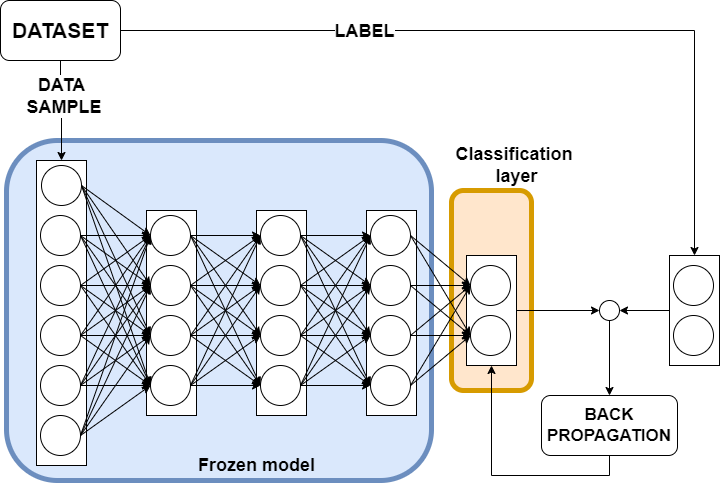
\includegraphics[width=120mm]{Figures/Chapter3/basicsystem.png} 
    \caption{Block diagram showing an example of model training}
    \label{fig:block_diag_esempio}    
\end{figure}

The basic formulas used for the propagation of errors in a classification layer are the following:

\begin{align} 
	z_i &= \sum_i w_{ij} \: x_j + b_i \label{zi} \\ 
	y_i &= Softmax(z_i) = \frac{e^{z_j}}{\sum_j=1^k e^{z_j}} 	\label{yi} \\
	L^{CROSS}_i &= - \frac{1}{n} \sum_k [\ y \: ln(y_i) \: +\: (1-t_i) \: ln(1-y_i) ]\ \label{cost_cross} \\
	where & \: \: i= 0,1..,n  \: \: and \: \:  j=0,1,..,m \nonumber 
\end{align}

Where equation \ref{zi} is the formula that describes the propagation of inputs through an ML node, equation \ref{yi} is the definition of the Softmax function, equation \ref{cost_cross} is the definition of the categorical cross-entropy loss function, $n$ is the number of classes known by the mode, and $m$ is the number of outputs of the grey box (or the number of nodes of the frozen model's last layer).\\
Knowing the entire mathematical description of the classification layer, it is possible to compute the relation between weights and prediction error. To do so, it is necessary to compute the derivative of the error with respect to the weight of interest. 

\begin{equation}
	\frac{\partial L^{CROSS}_i}{\partial w_{ij}} = \frac{\partial L^{CROSS}_i}{\partial S_i} \cdot \frac{\partial S_i}{\partial z_i} \cdot \frac{\partial z_i}{\partial w_{ij}}  
\end{equation}

Each block is then computed as:

\begin{align}
	\frac{\partial z_i}{\partial w_{ij}} &= \frac{ \partial (\ \sum_i w_{ij} \: x_j + b_i )\ }{ \partial w_{ij}} = x_i \\[10pt]
	%
	\frac{\partial S_i}{\partial z_i} &= \frac{e^{z_i} \sum e^{z_i} - e^{z_i} e^{z_i}}{ (\ \sum e^{z_i} )\ ^2} \nonumber \\
	&= \frac{e^{z_i}}{\sum e^{z_i}}- \frac{(e^{z_i})^2}{(\sum e^{z_i})^2} \nonumber \\
	&= Softmax(z_i) - (Softmax(z_i))^2 \nonumber \\
	&= Softmax(z_i) - (1-Softmax(z_i)) \\[10pt]
\end{align}

The steps required for the computations of the last block are a bit more complex:

%\begin{align}
%	S_i &= \frac{e^{z_i}}{\sum_i e^{z_i}} = \frac{e^{z_i}}{\omega} \qquad log(S_i) = z_i - log(\omega)\\
%	\frac{\partial L^{CROSS}_i}{\partial S_i} &= \frac{\partial (\ - \frac{1}{n} \sum_k [\ y \: ln(y_i) \: +\: (1-t_i) \: ln(1-y_i) ]\ )\ }{\partial S_i} \\
%	&= - \sum_j t_j \frac{\partial log(S_i)}{\partial S_i} \\
	
%	where & \frac{\partial log(S_i)}{\partial z_i}
%\end{align}

Then, it is possible to apply the relation weight-error inside a feedback loop for the correction of the parameters. The final formula that defines the back propagation on weights and biases of a classification layer that uses Softmax as activation function and categorical cross-entropy as loss function is:

\begin{align}
	w_{ij} &= w_{ij} - l_{rate} \cdot (\ y_i-t_i )\ \cdot x_j \label{w_update} \\
	b_i    &= b_i    - l_{rate} \cdot (\ y_i-t_i )\ \label{b_update} 
\end{align}

Where $w_{ij}$ is the weight in the position i,j of the matrix, $b_i$ is the i-th bias of the array, $l_{rate}$ is the learning rate, which is a parameter that defines how fast the correction modifies the weight, $y_i$ is the i-th value inside the array generated by the frozen model and $t_i$ is the i-th value of ground truth label. Note that the label in this case is a hot-one encoded array. This means that the array is filled with zeros and contains a 1 only in the position that represents the correct class.

\section{Implemented algorithms}
The study started from the implementation of the TinyOL strategy aforementioned for performing CL. Later the study was expanded to other state-of-the-art methods. As explained in Chapter \ref{chap:relworks}, regularization approaches are strategies that exploit the addition of loss terms in the update rule. Thanks to this, it is possible to have some control over the weight update. In today's research some strategies for CL training have been proposed mainly with the aim of contrasting catastrophic forgetting, but they were never applied to MCUs. The best performing state-of-the-art regularization strategies are Elastic Weight Consolidation (EWC), Synaptic Intelligence (SI), and Learn Without Forgetting (LWF) \cite{li2017learning}. In another paper, the authors propose a method called Copy Weight with Reinit (CWR) \cite{lomonaco2017core50}, which was later improved with the CWR+ version in paper \cite{maltoni2019continuous}, where also a new method, called AR1, was proposed. In this study, only some of the aforementioned strategies were implemented, namely LWF, CWR, and TinyOL, together with small variations that aim at using batches of data. \\
In these applications, the algorithms are applied with the same system. The framework substitutes the classification layer of a pre-trained model, called the frozen model. The frozen model is used only as a feature extractor which provides an array of elaborated data. All the implemented strategies are applied only on the classification layer.

\subsection{TinyOL}
The TinyOL method is suitable for MCUs, and was initially implemented in the paper \cite{ren2021tinyol}. The strategy is straightforward and follows the basic ML training step, which consists of computing the error from the prediction and propagating it on the weights and biases through stochastic gradients descend (SGD). Its implementation consists of a couple of $for$ loops for updating the biases and the weights. The weights update rule for this algorithm are:

\begin{align}
    w_{i,j} &= w_{i,j} - \alpha (y_i - t_i) \cdot x_i \\
    b_i     &= b_i - \alpha (y_i - t_i) \\
    where \:\: i &= 0,1..,n  \: \: and \: \:  j=0,1,..,m \nonumber 
\end{align}

Where $y_i$ is the i-th value in prediction array obtained from the OL layer, $t_i$ is the i-th value of the true label array, $\alpha$ is the learning rate (tuned by the user), $w_{i,j}$ are the weights of the OL layer, $b_i$ are the biases of the OL layer, $n$ is the max amount of classes known by the OL system, and $m$ is the height of the last layer of the frozen model. Note that the value $n$ can change dynamically in all strategies implemented because the maximum number of possible classes is not known a priori, or at least it is not known in a real-life application. \\
Also a variation of this method is proposed. The variation takes into consideration the possibility to apply a back propagation that depends on a group of samples (a batch) and not just from the last sample received. The idea for implementing such a variation came thanks to the article \cite{batch_size_medium}, where the author explores the impact that the batch size has on ML training dynamics. The base strategy of the variation is to compute a backpropagation that depends on a batch of inputs and not just from the last sample recorded. This helps the model to be less vulnerable to noisy data and outliers. To implement an algorithm with this variation, it is necessary to maintain in memory all the samples from the batch. This requires the allocation of double the amount of memory used for the standard version. This is done by allocating two additional matrices, one called W, which contains the data of old samples related to the weights, and the other one called B, which contains the data of old samples related to the biases. These matrices are used as a cumulative memory of the back propagation applied by each training step. Every time a new sample is received and elaborated, the upgrade of each weight and bias is computed and added in the correct spot inside matrices B and W. When a batch is finished, the average backpropagation update is computed and applied on the actual matrices of weights and biases. Note that during a batch the OL system performs an inference with the frozen model's output by using matrices w and b, computes the error, computes the back propagations to be applied on W and B, and adds the updates in matrices W and B. During an entire batch, the weights used for inference are kept constant. When a batch is finished the average is computed and the update rule is applied. Then, the content of W and B is deleted and restored to 0. \\
So, the update rule at each inference step becomes:

\begin{align}
	W_{i,j} &= W_{i,j} + \alpha (y_i - t_i) \cdot x_i \\
    B_i     &= B_i + \alpha  (y_i - t_i) 
\end{align}

And at the end of every batch the update applied on the real weights is:

\begin{align}
	w_{i,j} &= w_{i,j} - \frac{1}{batch\_size} \cdot W_{i,j} \\
	b_i     &= b_i - \frac{1}{batch\_size} \cdot B_i
\end{align}

Methods TinyOL and TinyOL with batches are based on the same basic principle which is quite simple. The method TinyOL requires the use of only one weight matrix and one bias array and their dimension depends on two parameters: the number of classes known by the OL system represented by the value $n$ and the size of the frozen model's last layer, represented by the value $m$. This makes the memory allocated from the method be equal to a total of $(n \times m+n \times 1)\times 4 \: bytes$. The method changes the layer parameters each time a new sample is received, with no constraints. The model learns from every single sample that it receives, no matter if the sample is noisy, an outlier or wrongly labelled. This aspect is the main problem that concerns the TinyOL strategy and makes it vulnerable to catastrophic forgetting. By allowing such a high flexibility to adapt to any kind of data, the model is not protected at all from catastrophic forgetting.\\
On the other hand, the method TinyOL with mini-batches exploits the same approach but applies a back propagation that is dictated by the average update computed from a group of $k$ samples. Depending on the value of $k$, the group can be a more or less good representation of the data received. In any case, this method can better contrast catastrophic forgetting, noisy data, and outliers. \\
Figures \ref{fig:block_diag_OL} and \ref{fig:block_diag_OLwb} contain a block diagram showing how the two methods behave.

\begin{figure}[h!]
    \centering
    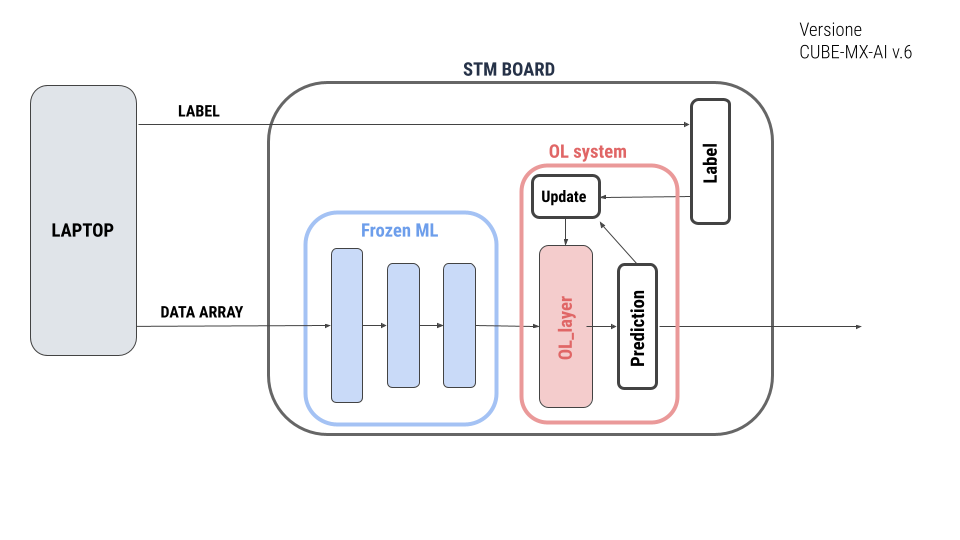
\includegraphics[width=120mm]{Figures/Chapter3/OL.png} 
    \caption{Block diagram describing the algorithm TinyOL.}
    \label{fig:block_diag_OL}    
\end{figure}

\begin{figure}[h!]
    \centering
    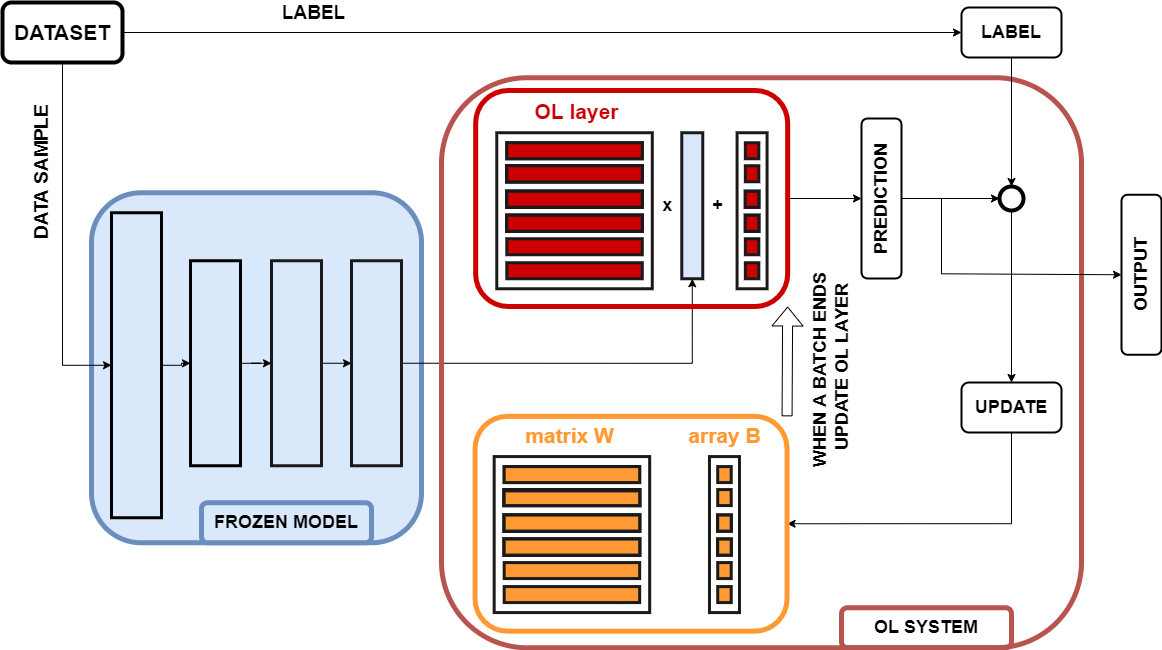
\includegraphics[width=120mm]{Figures/Chapter3/OLwb.png} 
    \caption{Block diagram describing the algorithm TinyOL with batches.}
    \label{fig:block_diag_OLwb}    
\end{figure}

\subsection{TinyOL V2}
To contrast catastrophic forgetting, a modified version of the original TinyOL method was developed, namely TinyOL V2. The idea is to contrast the drift that affects the original weights by completely removing the possibility to update those weights. The algorithm applies the same rule seen before, but only on the parameters that represent new classes. The update rules become:

\begin{align}
	w_{i,j} &= w_{i,j} - \alpha (y_i - t_i) \cdot x_i \\
    b_i     &= b_i - \alpha (y_i - t_i) \\
    where   & \: \: i= p,p+1..,n  \: \: and \: \:  j=0,1,..,m \nonumber  
\end{align}

The only difference with respect to the TinyOL method is the iterator $i$, which goes from $p$ to $n$, where $p$ represents the position of the first unknown class. \\
Also in this case, the variation that uses batches was implemented. Again, the method requires the use of two additional matrices called $W$ and $B$, which contain the cumulative backpropagation computed at each step. As before, the algorithm follows the same rules as TinyOL with batches, but with the iterator $i$ going from $p$ to $n$. The rule that defines the standard behaviour during training is:

\begin{align}
    W_{i,j} &= W_{i,j} + \alpha (y_i - t_i) \cdot x_i \\
    B_i     &= B_i + \alpha  (y_i - t_i) 
\end{align}

And at the end of every batch, the weights and biases are updated using the average backpropagation saved in matrices $W$ and $B$.

\begin{align}
    w_{i,j} &= w_{i,j} - \frac{1}{batch\_size} \cdot W_{i,j} \\
    b_i 	    &= b_i - \frac{1}{batch\_size} \cdot B_i \\
    where   & \: \: i= p,p+1..,n  \: \: and \: \:  j=0,1,..,m \nonumber  
\end{align}

As seen for the TinyOL with batches, TinyOL V2 with batches allows the model to learn from a bigger group of samples. This ability should help the model to avoid over fitting, outliers, and noisy data. \\
In conclusion, TinyOL V2 is a simple method that differs from the original strategy only because the update is restricted to the new parameters.  By forcing the update on just a portion of the weight and biases, the context drift, that would irreversibly modify the original weights and lead to catastrophic forgetting, is completely removed. This helps the algorithm in contrasting catastrophic forgetting but also reduces the ability of the model to perform fine-tuning on those classes. By having a training strategy that updates only a portion of weights, it is not possible to create a model that behaves as optimizer of the loss function. This means that at the end of the training, the model is composed of two parts that behave differently at every iteration. One portion of the weights behaves as the original model, while another part of the weights behaves as the most recent version of the model. These two parts, when computing a prediction, cannot make the model converge towards an optimized prediction. \\
The method TinyOL V2 requires the same amount of memory used by TinyOL, which means a matrix of size $n \times m$ and an array of size $n \times 1$. On the other hand, the method TinyOL V2 with batches requires an additional matrix and array with s reduced size of $(n-p) \times m$ and $(n-p) \times m$. Figures \ref{fig:block_diag_OLV2} and \ref{fig:block_diag_OLV2wb} contain block diagram showing the pipeline of the two methods.

\begin{figure}[h!]
    \centering
    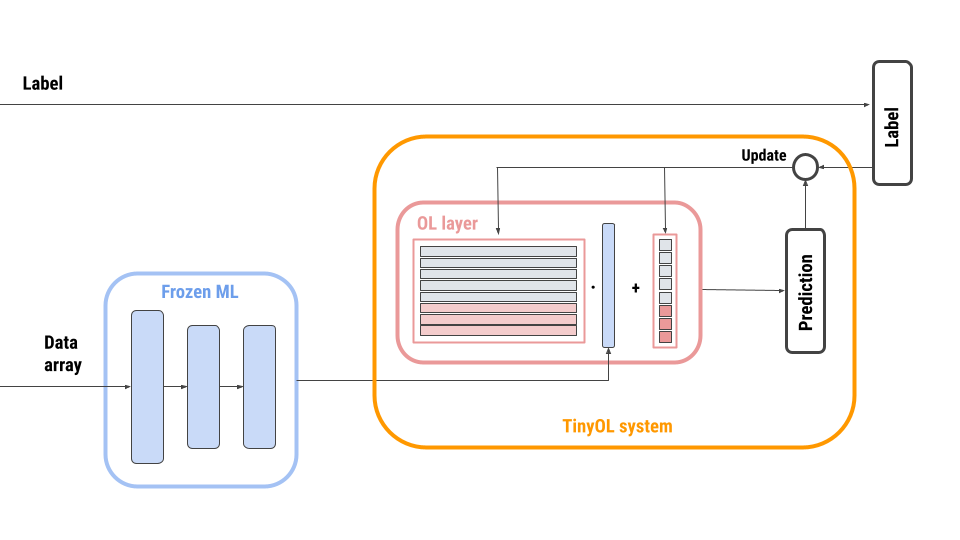
\includegraphics[width=120mm]{Figures/Chapter3/OLV2.png} 
    \caption{Block diagram describing the algorithm TinyOL V2.}
    \label{fig:block_diag_OLV2}    
\end{figure}

\begin{figure}[h!]
    \centering
    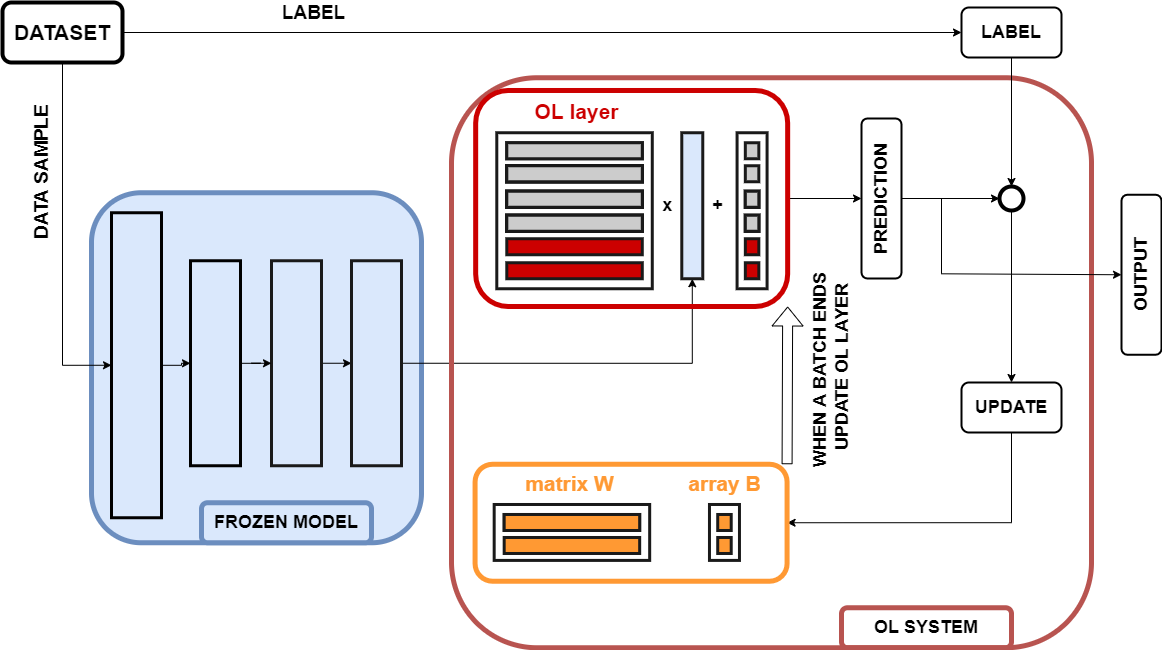
\includegraphics[width=120mm]{Figures/Chapter3/OLv2wb.png} 
    \caption{Block diagram describing the algorithm TinyOL V2 with batches.}
    \label{fig:block_diag_OLV2wb}    
\end{figure}

\subsection{LWF}
The LWF strategy is a regularization approach introduced in \cite{li2017learning} and later applied with a small variation in \cite{maltoni2019continuous}. The main idea of the method is to contrast catastrophic forgetting by applying a smart loss function paired with a double architecture (i.e., two ML models are required) used for combining old and new knowledge in the back propagations. Differently from the application in \ref{maltoni2019continuous}, this study applies the OL system only on the classification layer. This means that the double architectures is composed of only two classification layers and not two entire models. The first one is called the training layer, $tl$, while the second is called the copy layer, $cl$. The role of $tl$ is to be continuously updated at each training step with the particular $LWF$ backpropagation rule, while $cl$ is just a copy of the original frozen model's classification layer (computed by Tensorflow on the laptop training session). So the two layers represent opposite behaviours, $tl$ is the up-to-date model that evolves accordingly to the $LWF$ update rule while $cl$ represents the original model that remains constant and has no knowledge about new classes. \\
The backpropagation rule can be easily obtained by performing SGD on the $\mathcal{L}_{LWF}$ loss function expressed in Equation \ref{lwfcost}. The function aims at generating an update that depends on a dynamic average computed between the errors committed by both classification layers. Note that the $LWF$ strategy requires two predictions, which means also twice the computation. The final update rule can be easily obtained by computing the derivative of $\mathcal{L}_{LWF}$ with respect to the weights and biases. The result turns out to be just the average of the back propagations.

\begin{align}
	\mathcal{L}_{LWF} ( y_i, z_i, t_i) &=  (1-\lambda) \cdot{L}_{cross}(y_i, t_i) + \lambda \cdot{L}_{cross}(y_i, z_i) \label{lwfcost}\\
	w_{i,j} &= w_{i,j} - \alpha \cdot x_i \cdot [\ (y_i - t_i)(1-\lambda) + (y_i - z_i)\lambda ]\  \\
	b_i     &= b_i - \alpha \cdot [\ (y_i - t_i)(1-\lambda) + (y_i - z_i)\lambda ]\ \\
    where   & \: \: i= 0,1,..,n  \: \: and \: \:  j=0,1,..,m \nonumber  
\end{align}

Where $y_i$ is the i-th element of the prediction array obtained from the layer $tl$, $z_i$ is the i-th element of the prediction array obtained from the layer $cl$, $t_i$ is the i-th element of the ground truth label, and $\lambda$ is the variable weight that defines which prediction has more decisional power.\\
The back propagation is composed of two parts, the first is defined by $tl$ and the second is defined by $cl$. The value $\lambda$ plays a very important role in this update. As explained in \cite{maltoni2019continuous} its value cannot stay constant because it would be suboptimal. Their application used an evolution that followed a discrete function proportional to the number of batches encountered. In this case, $\lambda$ needs to be dependent on the number of samples encountered. The update of the loss function weight was found experimentally and is the following:

\begin{equation}
	\lambda = \frac{100}{100+ \text{prediction$\_$counter}}
\end{equation}

Another important aspect is that Equation \ref{lwfcost} follows the variation proposed in \cite{maltoni2019continuous}, where the loss functions $\mathcal{L}_{LWF}$ is not a sum between $categorical$ $cross$ $entropy$ and $knowledge$ $distillation$, but a sum of two $categorical$ $cross$ $entropy$. This is a little modification that allows for an easier implementation without dropping in performance. \\
Also in this case a version for integrating upgrades depending on batches is proposed. This time the method does not maintain the $cl$ constant for the entire training, but rather updates its values every time a batch is finished. At this point, the algorithm becomes a fusion between new knowledge and knowledge coming from an old version of the layer. The size of a batch is defined by the value $k$ and this value defines how old $cl$ is. The update rules in this case are:

\begin{align}
	w^{TL}_{i,j} &= w^{TL}_{i,j} - \alpha \cdot x_i \cdot [\ (y_i - t_i)(1-\lambda) + (y_i - z_i)\lambda ]\ \\
	b^{TL}_i     &= b^{TL}_i - \alpha \cdot [\ (y_i - t_i)(1-\lambda) + (y_i - z_i)\lambda ]\ \\
	where        & \: \: i= 0,1,..,n  \: \: and \: \:  j=0,1,..,m \nonumber  
\end{align} 

And at the end of one batch (once every $k$ values are elaborated) the parameters of $cl$ are updated in the following way:

\begin{align}
	w^{CL}_{i,j} &= w^{TL}_{i,j}  \\
	b^{CL}_i     &= b^{TL}_i  
\end{align}

Where $w^{CL}_{i,j}$ and $b^{CL}_i$ are respectively the weights and biases of $cl$, while $w^{TL}_{i,j}$ and $b^{TL}_i$ are the weights and biases of $tl$.\\
This method also requires a different $\lambda$ rule. Experimentally it has been found the following rule to be well working:

\begin{equation}
\lambda = \left\{
        		\begin{array}{ll}
            		1                                                         & prediction \_ counter \leq batch \_ size \\
            		\frac{\text{batch$\_$size}}{\text{prediction$\_$counter}} & prediction \_ counter >    batch \_ size
        		\end{array}
    		  \right.
\end{equation}

Both LWF methods require the same amount of memory, which is two times the amount required for a classification layer, so $(\ n \times m )\ \times 2$ and $(\ n \times 1 )\ \times 2$. Both methods are quite easy to implement. Their strength is defined in the value $\lambda$ and in the particular update rule. The two methods differ only because of the update on $cl$. A negative aspect that characterizes these two methods is the amount of computation required, which can be a problem for tiny devices. Having two layers and the need for two predictions is of course needed to double the computation. Figure \ref{fig:block_diag_LWF} contains a block diagram that explains the pipeline of the LWF method.

\begin{figure}[h!]
    \centering
    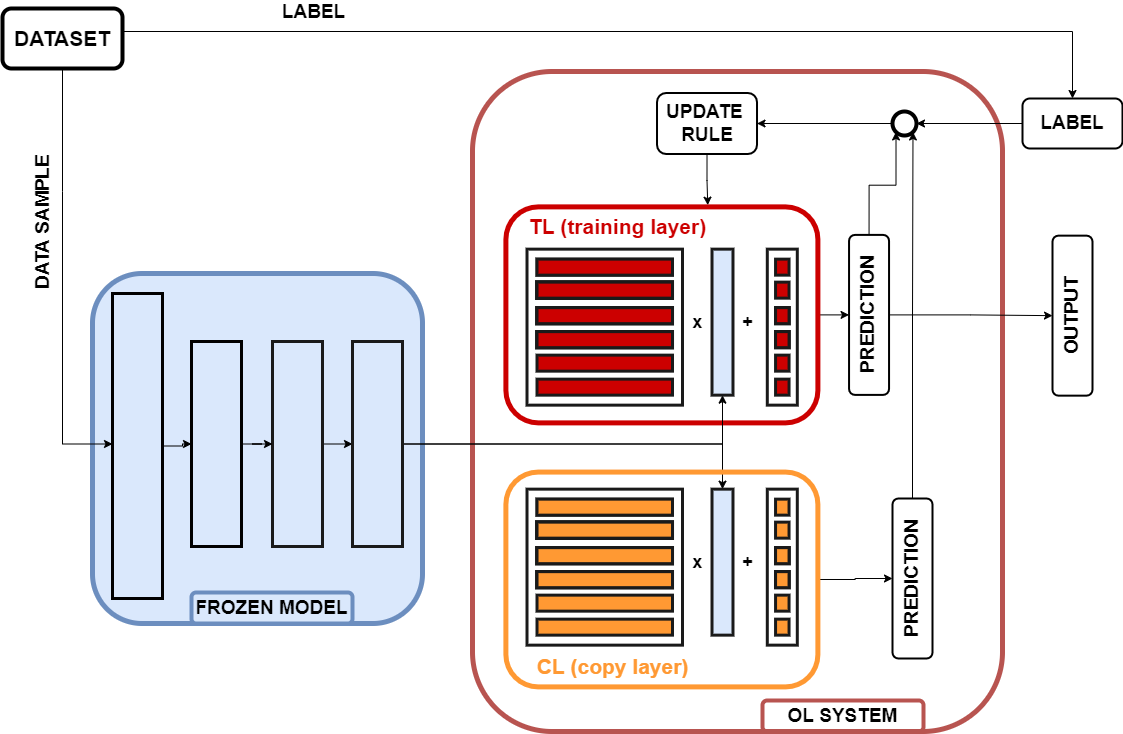
\includegraphics[width=120mm]{Figures/Chapter3/LWF.png} 
    \caption{Block diagram describing the algorithm LWF.}
    \label{fig:block_diag_LWF}    
\end{figure}

\subsection{CWR}
CWR is an architectural approach that exploits the usage of two classification layers and a weighted back-propagation rule for performing OL. Again, the two classification layers are called training layer, $tl$, and consolidated layer, $cl$. The idea for this algorithm is to train the two layers in two different ways. For $tl$, the same strategy used in TinYOL is applied. On the other hand, $cl$ is updated once every batch with a particular update rule. The back propagations for $tl$, that is computed at every step is:

\begin{align}
	w^{TL}_{ij} &= w^{TL}_{ij} + \alpha (y^{TL}_i - t_i) \cdot x_i \\
    b^{TL}_i    &= b^{TL}_i + \alpha  (y^{TL}_i - t_i) 
\end{align}

While, the backpropagation for $cl$, that happens once every batch, is the following:

\begin{align}
	w^{CL}_{ij} &= \frac{w^{CL}_{ij} \cdot updates_{i} + w^{TL}_{ij}}{updates_{i} + 1} \label{cwrweight}\\ 
	b^{CL}_{i}  &= \frac{b^{CL}_{i} \cdot updates_{i} + b^{TL}_{i}}{updates_{i} + 1} \\ 
    w^{TL}_{ij} &=  w^{CL}_{ij} \\
    b^{TL}_{i}  &=  b^{CL}_{i} 
\end{align}

Where $w^{TL}_{ij}$ and $b^{TL}_i$ are the weights and biases of the training layer, $w^{CL}_{ij}$ and $b^{CL}_i$ are the weights and biases of the consolidated layer, $updates_{i}$ is an array that behaves as a counter of labels encountered, $y^{TL}$ is the prediction obtained from $tl$, and $\alpha$ is the learning rate.\\
The use of two classification layers that update in this way makes the framework behave as a system composed of a short-term memory and a long-term memory. Because of the continuous update at every batch, $tl$ is the short-term memory. This layer learns from every single sample that is received, and at the end of a batch, it gets corrected with the parameters from $cl$. On the other hand, $cl$ behaves as the long-term memory. This is because it never gets reset or cleaned and it gets updated only once every batch with information coming from the short term memory. Note that the weighted average method depends on the number of times that a specific label appeared in the training batch.\\
Another important aspect of this method regards the amount of computations required at each step. While training, the method requires only to perform one inference from $tl$. In fact no predictions from $cl$ are actually useful at any point during training. The inference obtained from $cl$ can be performed only when actively requested. Considering that $cl$ represents the long term memory, its prediction considered the most reliable and generally the most accurate between the two. For this study case, inferences from $cl$ are required only during the testing that is performed at the end of the training. In real-life scenarios these predictions should be performed only when actively requested. This is because the amount of computation required for one step is doubled, and the only improvement obtained would be the info given to the user.\\
CWR is an easy-to-implement method. Its strengths are hidden in the double architecture and the update rule that make possible the merging of short-term memories and long-term memories. The amount of memory required for this algorithm is two weight matrices of size $n \times m$, 2 bias arrays of size $n \times 1$, and one array that keeps track of the labels encountered of size $n \times 1$ (is called updates in equation \ref{cwrweight}). The amount of computations can change if an inference is required, making it double. Figure \ref{fig:block_diag_CWR} contains a block diagram that shows the pipeline of the CWR algorithm.

\begin{figure}[h!]
    \centering
    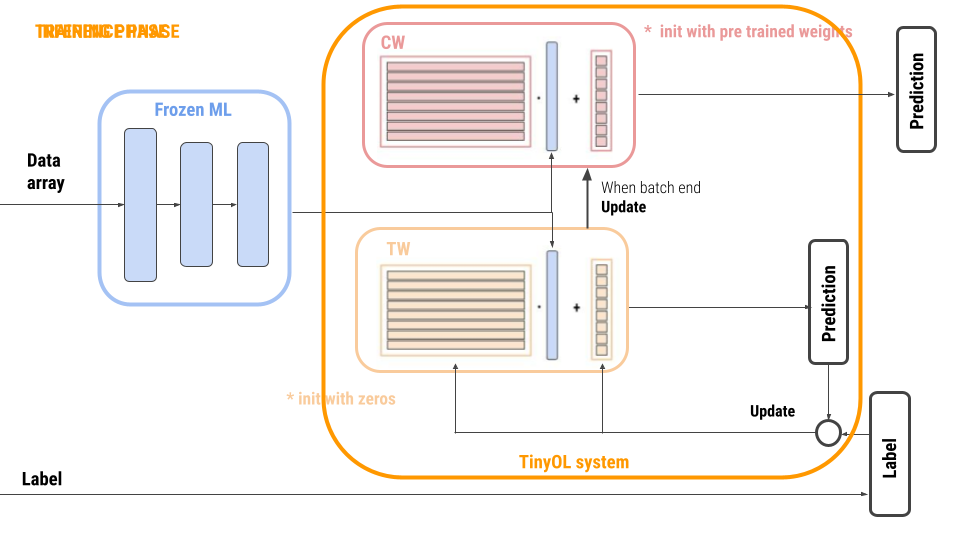
\includegraphics[width=120mm]{Figures/Chapter3/CWR.png} 
    \caption{Block diagram describing the algorithm CWR.}
    \label{fig:block_diag_CWR}    
\end{figure}

\subsection{My algorithm}




% INSERIRE MODELLO ESEMPIO

And


\section{Gesture recognition application}

\section{Image classification application}





\chapter{Experimental setup}

In this chapter, the practical aspects of the experiments are described. Initially, the study was developed entirely on the laptop using Python code with the aim of understanding the theoretical behaviour of the methods and the capabilities of CL. Later, the same principle and basic pipeline were ported to the STM Nucleo and the OpenMV camera, respectively. All applications use the same general workflow: i) train the base model on a powerful device for the classification of the basic classes using Tensorflow; ii) manipulate and compress the model if necessary, then load it on the MCU of interest; iii) attach the OL system to the frozen model, then define the basic training parameters and the desired CL strategy. \\
In this chapter, all the most important steps for a good setup of the experiments are described. Specifically, these steps are: the dataset collection, the training of the frozen models, the implementation of the OL system on the MCUs, and the application of the entire system on the device with a short explanation of how the CL trainings are performed.

\section{Dataset collection}
To create and train ML models, it is necessary to have big datasets. In this study, the two applications explored elaborate two types of data. The Nucleo F410-RE application uses time series of data recorded from an accelerometer, while the OpenMV application uses images containing digits from the MNIST dataset \ref{deng2012mnist}. \\

\subsection{Accelerometer dataset}
For the gesture recognition application the dataset was created from scratch. Datasets of this type, containing accelerometer data representing gestures are not very common, so it was necessary to collect it. It was decided to collect time series of 3D accelerometer data of letters written in the air from the user as a proof of concept of a gesture recognition system.
The dataset collection was carried out with the hardware described in Chapter \ref{chap:hardware}. \\
The dataset is composed of 8 different letters, which are A,E,I,O,U and B,R,M. The vowels compose the original classes that are first learned by the frozen model, while the three consonants are the additional classes that are learned later by the CL system. The collection of the dataset is performed by connecting the MCU to a laptop via UART protocol (USB cable). The laptop behaves as a power provider and real-time storage for the data stream. 
To collect the sensor data, it is used a small script that controls UART and I2C communication with some timers and GPIOs. When the Nucleo detects a GPIO interrupt, the user specifies the label. Then the code records data from the sensors with a frequency of 100 Hz for 2 seconds. Meanwhile, the values are also streamed via USB to the laptop which stores data using a serial communication software (MobaXTerm). \\
To make the dataset be composed of samples that better resemble real-life applications, a NIC scenario was artificially imposed. This means that the recorded samples contain both new classes (the consonants) and new pattern of known classes. The latter was introduced by performing motion paths with accentuated characteristics. Some examples are: the accentuated oval shape of the letter O, the speed at which the sensor moves for the letter I, the general size/width/height of all letters, and the radius of the curves for letter R and B.
Figure \ref{fig:letters_motion} shows the general path that was followed while drawing the letters in the air.\\

\begin{figure}[h!]
    \centering
    
\includegraphics[width=120mm]{Figures/Chapter4/letters_motion.jpg} 
    \caption{Motion followed with the sensor for writing letters in the air.}
    \label{fig:letters_motion}    
\end{figure}

All the samples received by the MCU are saved in a table format in a text file. The columns of the table contain: the number of samples recorded, the label of the sample and three columns for the accelerations recorded from X, Y, Z axis. Considering that the MCU was set to work at a sampling frequency of 100 Hz for 2 seconds a single sample is composed of 600 values (200 for each axis). 
The final shape of the dataset is 5130 samples, where the vowels have on average 560 samples each, while the consonants have around 760 samples each. \\
Once the dataset is collected, post-processing is performed. This consists of a simple reshape, shuffle and subdivision. To perform the training on the ML architecture, all samples are reshaped by stacking all the rows into a single array from a matrix $3 \times 300$ to an array $1 \times 600$. Then, a subdivision of the dataset is performed. Given that the dataset is needed for two trainings (frozen model training and CL training), it is required to separate it correctly. The frozen model can recognize only vowels, thus its dataset is composed only of vowels. This dataset counts a total of 881 samples with 176 samples from each vowel. The OL model, on the other hand, is trained on all letters, so its dataset contains the remaining vowels and all the consonants. \\
After this, both datasets are divided in training and testing portions, which is done with the usual 80-20\% rule. Figure \ref{fig:flow_dataset_letters} shows how the dataset are divided and balanced for the two trainings regarding the gesture recognition application.

\begin{figure}[h!]
    \centering
    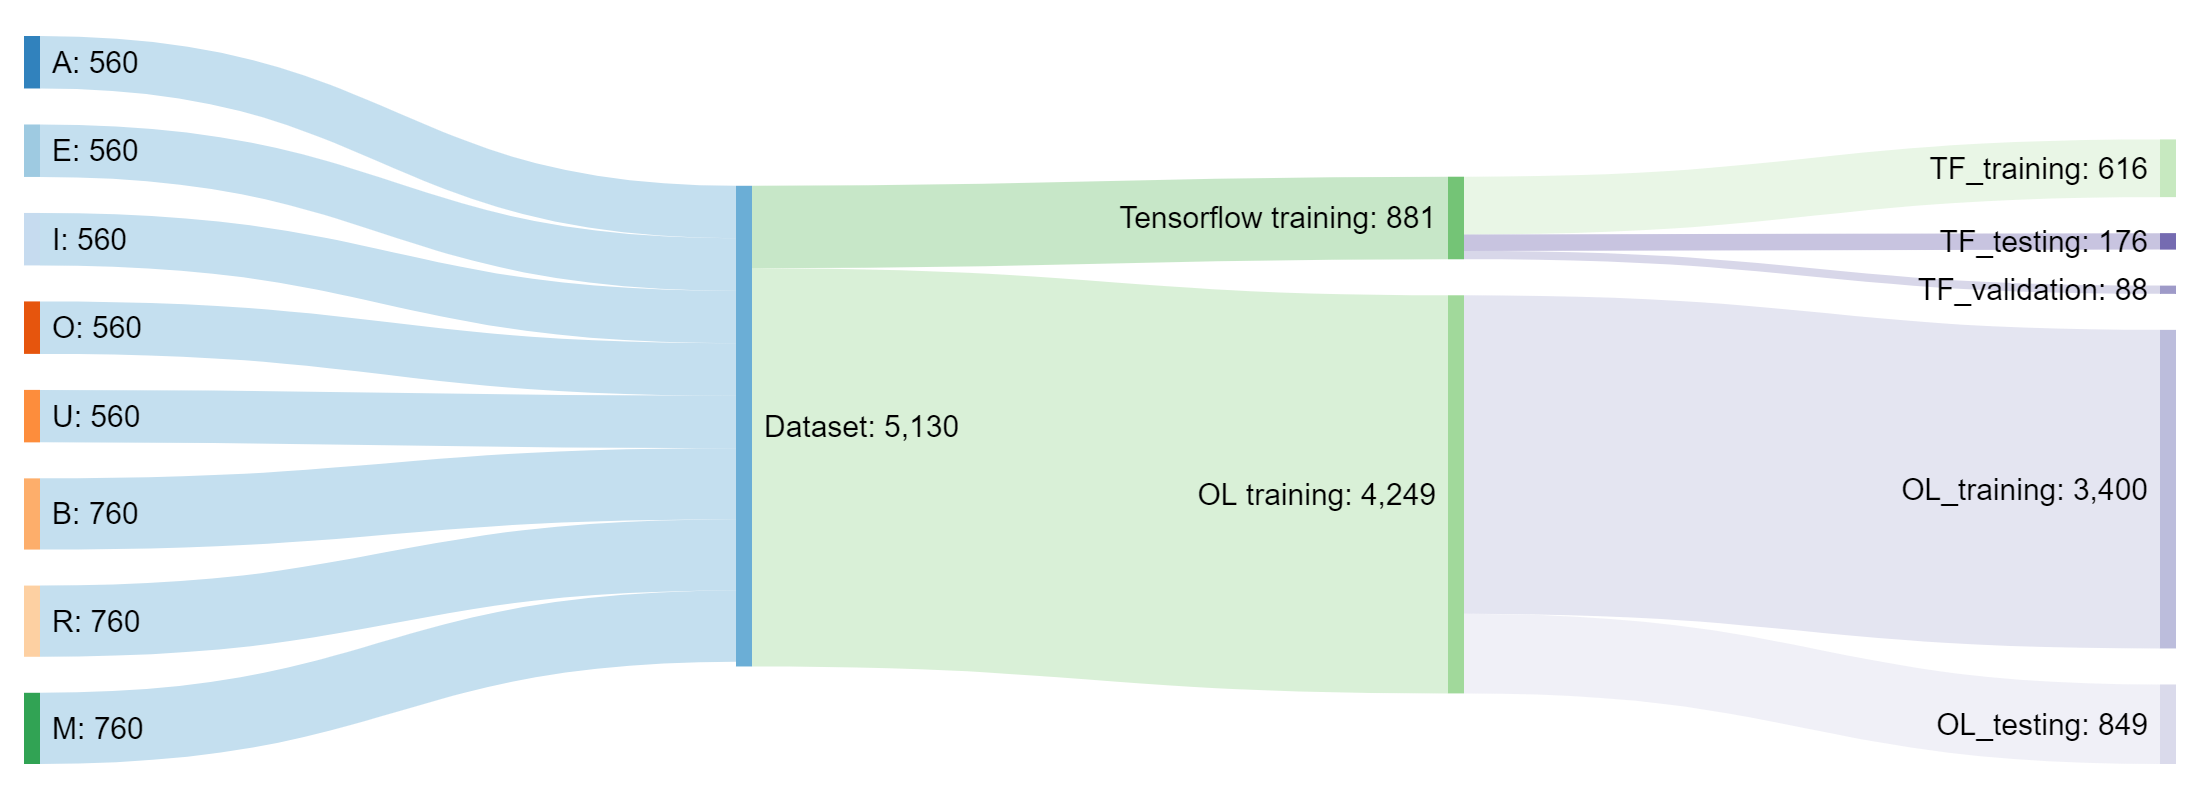
\includegraphics[width=120mm]{Figures/Chapter4/flow_dataset_letters.png} 
    \caption{Stankey diagram showing how the letter dataset is divided}
    \label{fig:flow_dataset_letters}    
\end{figure}

\subsection{Digits recognition dataset}
For the image classification application the well-known MNIST dataset was used. The MNIST dataset is a publicly available large collection of images of handwritten digits. The dataset is well known in academic and research for its small size of images and large quantity of samples. It is composed of 60000 images for training and 10000 images for testing. The images are gray scaled and have a size of $28 \times 28$ pixels. In today's research, the dataset is commonly used for benchmarking ML training, while in academic it is used for basic training of classification and generative models. Figure \ref{fig:mnist_dataset} contains some sample images that of the MNIST dataset.\\

\begin{figure}[h!]
    \centering
    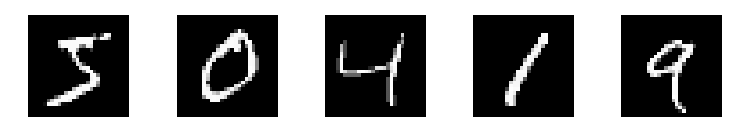
\includegraphics[width=100mm]{Figures/Chapter4/mnist_dataset.png} 
    \caption{Example of images from the MNIST digits dataset}
    \label{fig:mnist_dataset}    
\end{figure}

For this application purpose, the dataset requires pre-processing. Considering that the goal of the frozen model is to correctly recognize the digits from 0 to 5 it is necessary to separate the dataset into two groups, $low\_digits$ and $high\_digits$. By doing this, the $low\_digits$ group is composed of 36017 samples, while the $high\_digits$ group is composed of 23989 samples. For the training of the frozen model, the entire $low\_digits$ group is used for a Tensorflow training, which is further also separated in train, test, and validation. For this reason, the common 70-20-10 rule was used. On the other hand, for the training of the CL model only 5000 samples from the $high\_digits$ group were used. This because from the experience previously obtained from the latter application, it was demonstrated that 500 samples for each class are more than enough for a correct CL session. The CL dataset is then separated in training and testing with the rule 80-20\% for the CL application. \\
Figure \ref{fig:flow_dataset_openmv} shows how the dataset is divided for the training of the frozen model and CL model.

\begin{figure}[h!]
    \centering
    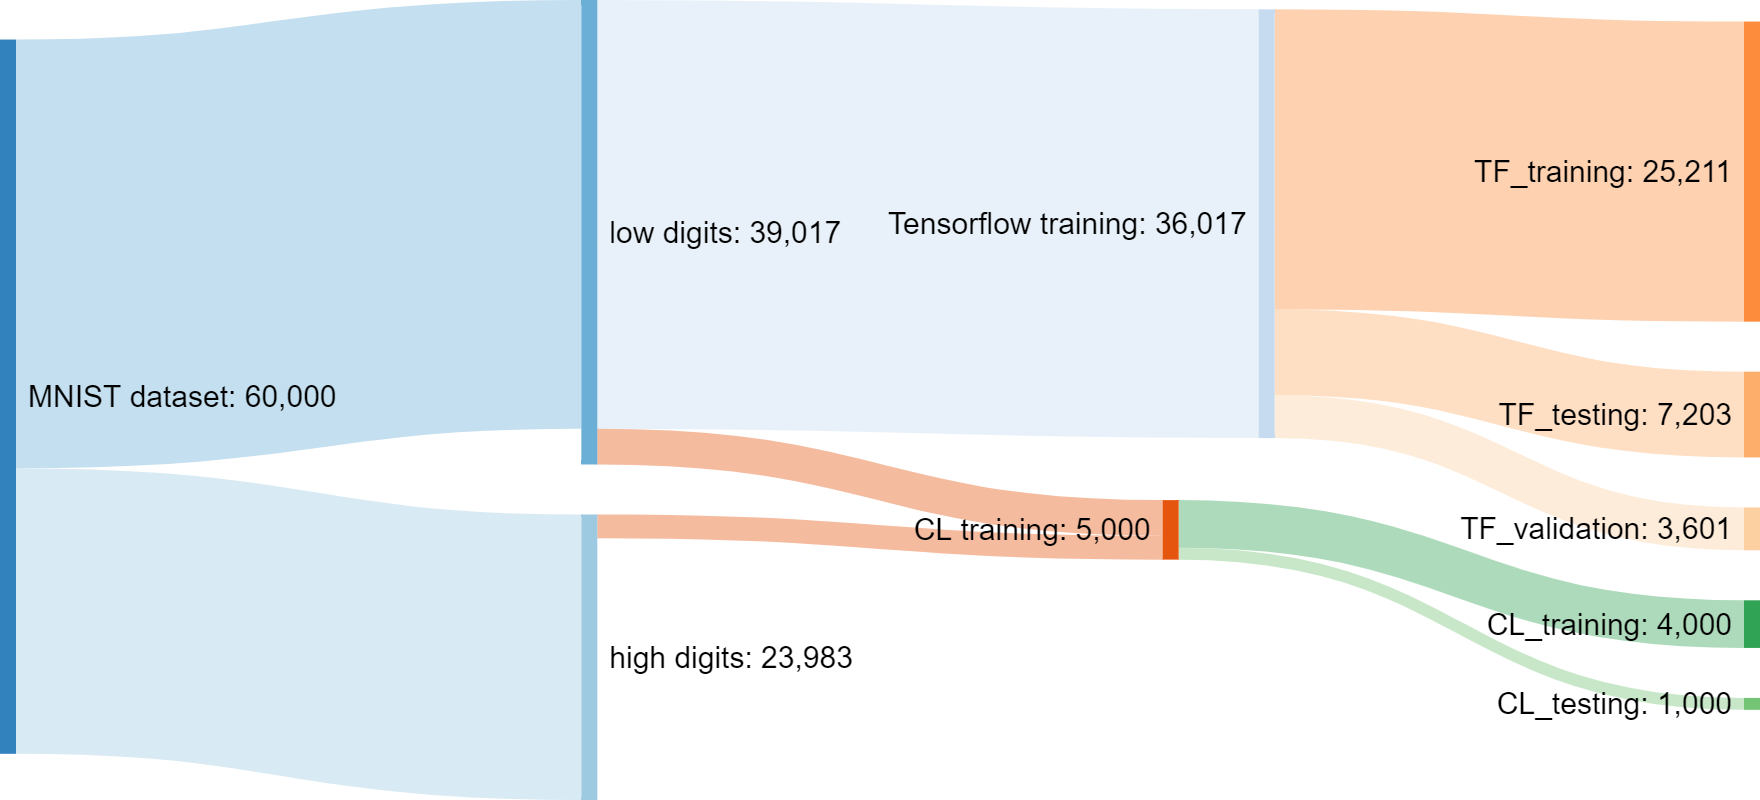
\includegraphics[width=120mm]{Figures/Chapter4/flow_dataset_openmv.png} 
    \caption{Stankey diagram showing how the MNIST dataset is divided}
    \label{fig:flow_dataset_openmv}    
\end{figure}

\section{Frozen model training and evaluation}
Once the datasets are created and post-processed, the training of the frozen models can be performed. Both models require small structures in order to be loaded on small MCUs. In both applications the models perform a classification, which can be achieved simply by imposing the last layer's activation function as a Softmax. All the other layers are used only for feature extraction and their structure and characteristics depend on the type of data to elaborate.
The trainings of the frozen models and their manipulation was carried out with Tensorflow library and Python.\\

\subsection{Gesture recognition model}
In the gesture recognition application, the model elaborates a time series of accelerometer data. The model's structure is composed of only fully connected layers, which makes the structure very simple. Typical applications of ML on time series use LSTM types of models, which are structures well suited for the elaboration of time dependent signals. In this case, the results obtained from a structure composed of only fully connected layers brought to satisfying results, so the model's structure was kept as is. The layer sizes are 600 for the input, 128 for the hidden layers, and 5 for the classification layers. The activations functions are, Softmax for the classification layer, and ReLU for all the other layers. Figure \ref{fig:letter_structure} shows a plot that contains the basic structure of the model used.\\

\begin{figure}[h!]
    \centering
    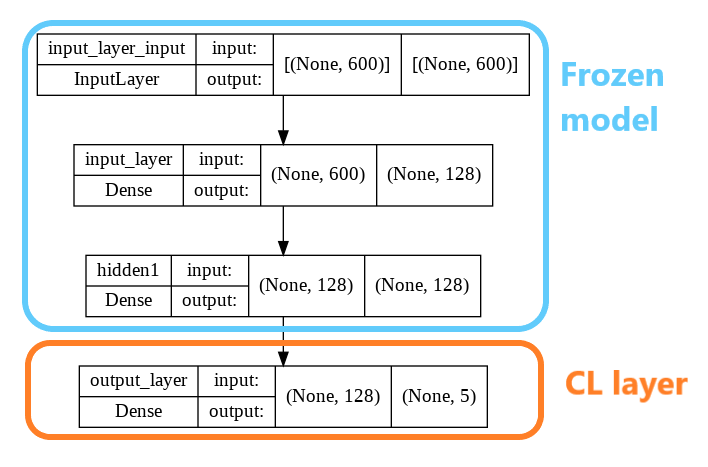
\includegraphics[width=120mm]{Figures/Chapter4/letter_structure.png} 
    \caption{Letter recognition model: basic structure and its separation in frozen model and OL classification layer}
    \label{fig:letter_structure}    
\end{figure}

The output layer's shape consists of 5 nodes because the model predicts 5 classes (the vowels). The number of layers and total parameters is quite low (94,085) respect to typical machine learning models; this makes it very suited for applications on MCUs. \\
The main training parameters are: $Adam$ optimizer, $categorical$ $cross$ $entropy$ as loss function, 20 epochs, and a batch size of 16. 
The accuracy obtained from the testing is 96.83\%. Figure \ref{fig:training_letters} contains two plots. On the left is shown the variation of the accuracy and loss during training, while on the right is shown the accuracy of each class at the end of the Tensorflow training.\\

\begin{figure}[h!]
    \centering
    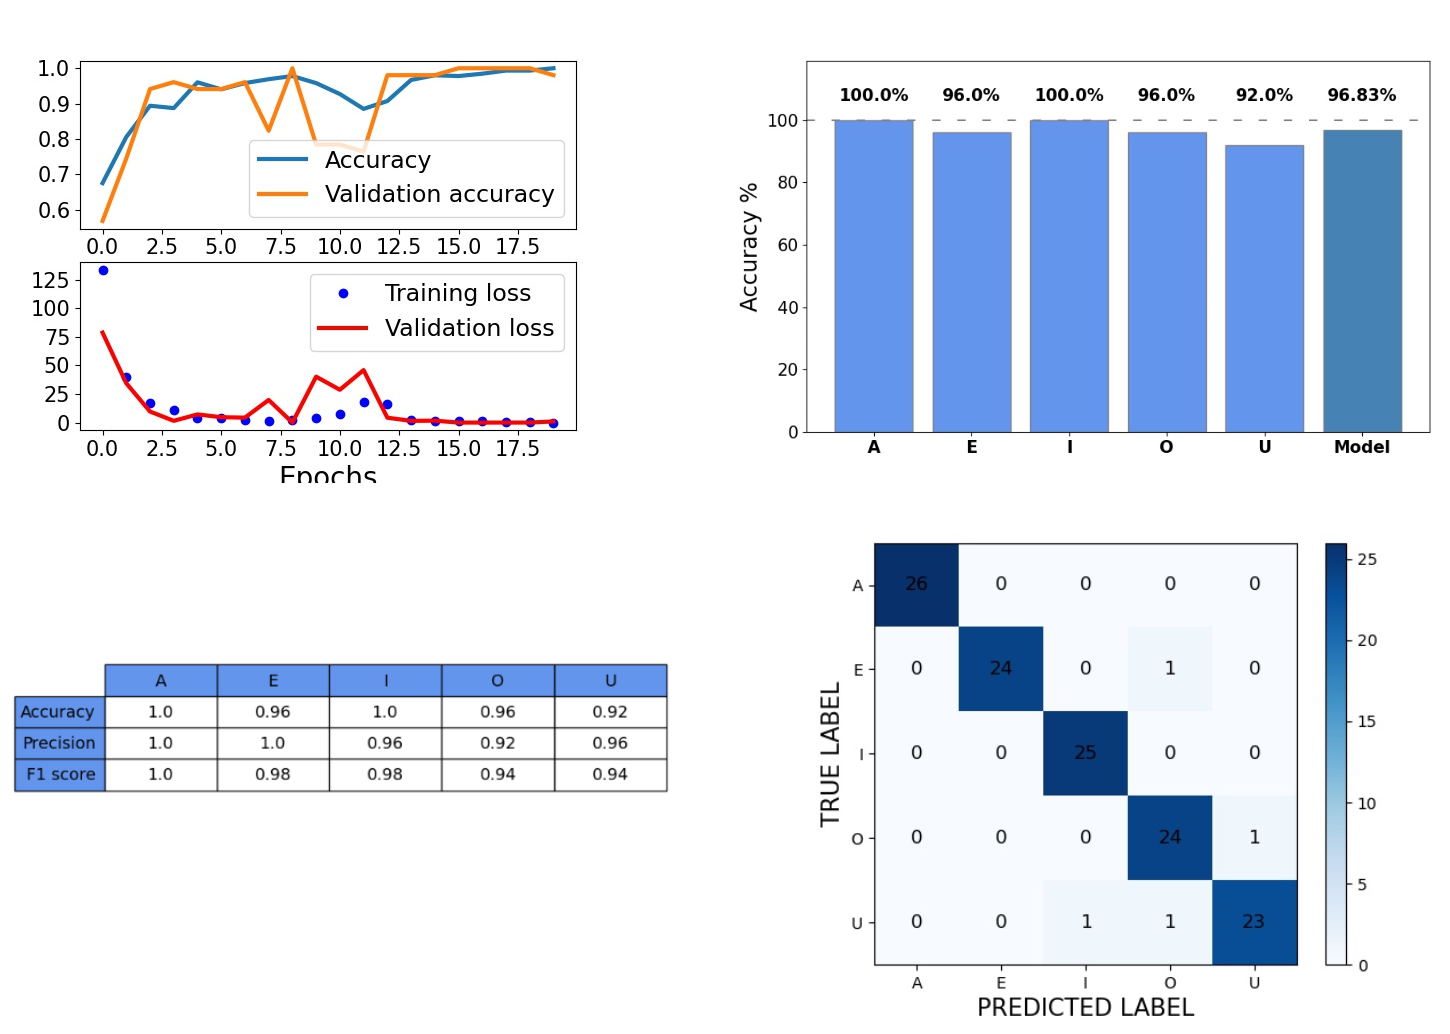
\includegraphics[width=130mm]{Figures/Chapter4/training_letters.png} 
    \caption{Results after the Tensorflow training. Top right: variation of accuracy and loss during training and validation. Top right: accuracy of the model in each class. Bottom left: table resuming precision accuracy and F1 score. Bottol right confusion matrix.}
    \label{fig:training_letters}    
\end{figure}

The last step consists of the preparation of the frozen models and the exportation of the model itself. This is necessary because of the particular actions that are performed on the last layer by the OL system. Because it is required to have total control over the weights and biases of the classification layer, it is necessary to have the model separated into two parts. The first one is called the frozen model and is just a $model.h5$ file which contains the truncated version of the trained model (classification model is removed). This portion of the model, once loaded on the MCU, is manipulated by the inference tools and can be used as a grey box. The output of this grey box is just the results from the feature extraction and it can be forwarded in the classification layer for the prediction.
The second part of the model exportation is the classification layer. The weights and biases of this layer are not exported as before, but are saved in a text file in matrix form. By doing this, it is possible to later load them in the MCU's RAM, which allows the OL system to edit and manipulate parameters and the layer shape. 
Figure \ref{fig:letter_structure} shows how the base model was divided into two main parts.

\subsection{Image classification model}
In the image classification application, a Convolutional Neural Network (CNN) architecture was used. These model types are specifically created for the elaboration of images and their main feature is the presence of convolutional layers for the feature extraction followed by NN layers for the classification. Figure \ref{fig:openmv_structure} contains a plot that shows the structure of the model.\\

\begin{figure}[h!]
    \centering
    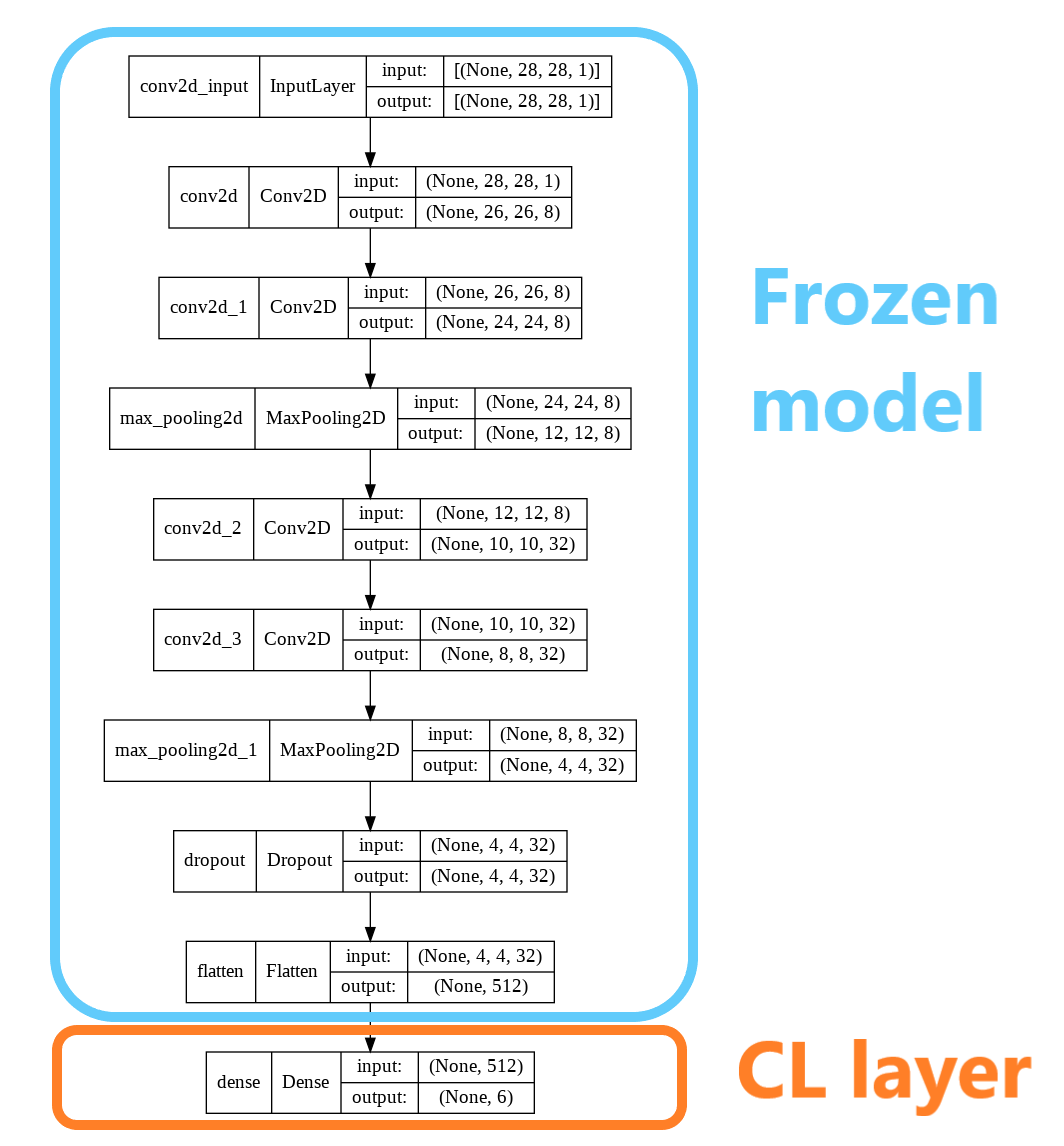
\includegraphics[width=100mm]{Figures/Chapter4/openmv_structure.png} 
    \caption{Image classification model: basic structure and its separation in frozen model and OL classification layer}
    \label{fig:openmv_structure}    
\end{figure}

The model contains two sequential blocks of two convolutional layers followed by Max Pooling. This type of structure allows the ML model to perform initially a feature extraction over the image and to flatten the output matrix to an array. The fully connected layer is used to elaborate the array and later feed the data to the classification layer, where the Softmax activation function is used for providing the probability of each class.\\
The output consists of 6 classes because the frozen model is trained for the recognition of the $low\_ digits$ group of images (i.e. digits from 0 to 5). Note also how despite having a more complex structure the number of parameters in the model is not much higher when compared to the previous application. This allows to have a small model that can be easily deployed on constrained MCUs for enabling fast inference. \\
The relevant training characteristics are: $Adam$ as optimizer, $categorical$ $cross$ $entropy$ as loss function, 30 epochs, and batch size of 64. The final accuracy obtained from the testing of the model is of $99.35\%$. Figure \ref{fig:training_mnist} shows on the right the behaviour of the accuracy and loss during training, and on the left the accuracy of the model for each class of the starting dataset.

\begin{figure}[h!]
    \centering
    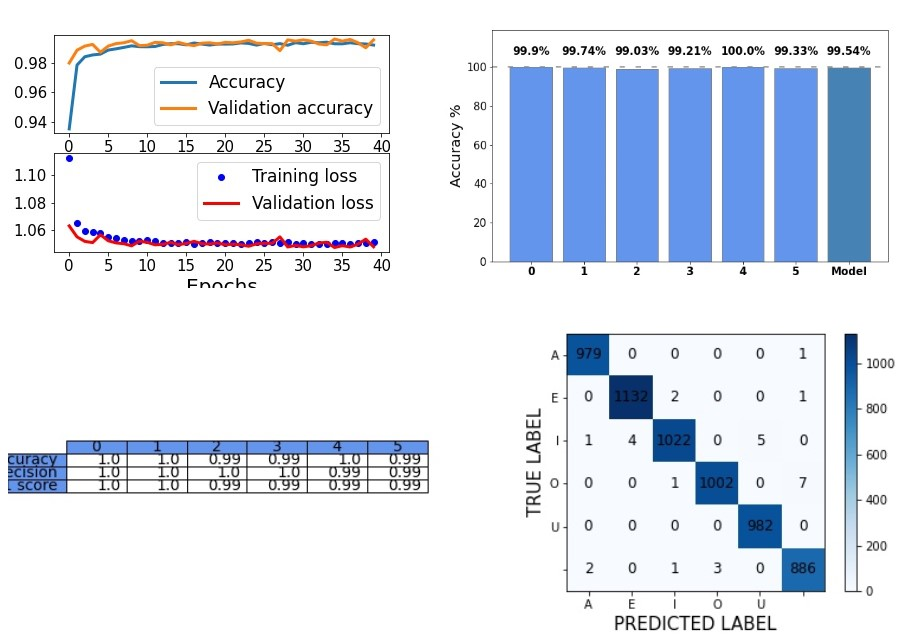
\includegraphics[width=130mm]{Figures/Chapter4/training_digits.jpg} 
    \caption{Results after the Tensorflow training. Top right: variation of accuracy and loss during training and validation. Top right: accuracy of the model in each class. Bottom left: table resuming precision accuracy and F1 score. Bottol right confusion matrix.}
    \label{fig:training_mnist}    
\end{figure}

Another important step that was performed for the OpenMV application is the pruning and quantization of the model. Usually, to deploy models with a high memory footprint it is necessary to apply compression techniques such ass combination of pruning and quantization.
Pruning is a method that reduces the number of connections in a NN model by setting to 0 redundant or non-relevant weights. This helps to reduce the memory occupied by the model, and if done strategically, can reduce the number of computations required for inference. By injecting forced sparsity inside the weight matrix, it is possible to reduce the computations needed, thus improving the inference efficiency. \\
Note that the Flash memory of the OpenMV is capable of storing models with bigger sizes than the one created, so pruning and quantization are not actually required. However, to demonstrate these model capabilities, it was decided to apply compression techniques anyway. The pruning and quantization procedure was carried out with Tensorflow, which makes the process as easy as a training setup. The main characteristics of the pruning are: $Adam$ as optimizer, $categorical$ $cross$ $entropy$ as loss function, 5 epochs, batch size of 32, initial sparsity of 0.5 and final sparsity of 0.8. After pruning the model shows an accuracy of $99.6\%$.\\
After this step, it is also possible to introduce the quantization operation. This is carried out almost automatically by Tensorflow simply by calling the correct functions. The model size along the different steps of the compression are: 230 kB after the first Tensorflow training, 86 kB after pruning and 64 kB after quantization. \\
As in the previous application, the last step consists of the exportation of the model. The frozen model is exported as $model.h5$, while the classification layer parameters are exported in text file and later loaded in the MCU. 

\section{STM F401-RE setup for gesture recognition}
In this section, the setup needed for a correct gesture recognition application is described. Specifically, it is described how the CL system was implemented on the Nucleo board, hoe the ML model was deployed on the MCU and how the communication laptop-MCU works.\\
In the gesture recognition application two software are exploited to add ML capabilities to the microcontroller. The first, STM-CUBE-MX, is a piece of software used for automatically generating chunks of code. This helps the user by lifting a lot of work required for the initial setup of the device. Thanks to this software, it is possible to use the UI and easily define the main characteristics of the MCU that is being programmed, starting from the definition of the main clock and the essential characteristics of all the peripherals enabled to the parameters of the communication protocols. The second piece of software is just an extension pack of STM-CUBE-MX, namely STM-CUBE-AI. This toolkit enhances capabilities of the MCU by adding the possibility to use machine learning models on the device. The main advantages brought by the extension pack are the possibility to automatically load and process ML models on the flash memory and run optimized routines for inference on the same model. This toolkit also allows the user to compress the model at deploy time. In this case, no compression is applied and the model is loaded as a $model.h5$ file.\\
Once the ML abilities have been added to the MCU it is possible to incorporate the CL system inside the code. The system, as already explained in Chapter \ref{basic_system}, is attached at the end of the frozen model, and it is composed mainly of functions for the elaboration of the frozen model's output, management of memory, and management of data stream. The entire system is written in C code and it is almost entirely contained in one single library. The entire project is available on GitHub \cite{github_repo}.\\
The basic structure of the code applied on the MCU is the following. At first, the most important parameters and variables are created. Depending on the algorithm defined, the right amount of memory is allocated. The weight and bias matrices are then filled with the parameters that have been previously generated by the Tensorflow training. Note that for the application on the Nucleo development board, the file is actually a C library which contains all the weights and biases written inside a matrix. Then the infinite while loop begins, and if the "received sample flag" is triggered, the frozen model inference is performed. Once the feature extraction is done, the output is fed to the OL layer, which will: propagate it through the classification layer, compute the prediction, compare the prediction with the label, compute the error, and back propagate the error on the weights using the adopted strategy. After this, a small message (32 bytes) containing the most relevant informations about the training step is generated and sent back through UART.\\
Once the CL system and the ML model are loaded correctly on the MCU, the experiment can begin. To perform a fast, reliable, and repeatable experiment, it was decided to develop a small app that controls autonomously the data stream towards the MCU. The app was developed in Python and is executed from the laptop, which stays in sync with the MCU and sends through UART (USB cable) one sample at a time. The script is quite simple and it follows the logic line: load the dataset of accelerometer array data, open the serial port with the specified properties, initialize containers for storing information, and start an infinite while loop where the communication laptop-MCU is continuously repeated. \\
When the app is launched, the MCU should already be connected to the laptop, otherwise the serial port cannot be opened. Once the script is launched and the initial setup is done, the app waits for an acknowledgement from the MCU (a message of 2 chars), which signals to the laptop that the device is ready to receive data and start the training. Once the ACK (acknowledgement) signal is received, the app sends a sample from the dataset composed of an array of 600 values and the label. The MCU then performs the routine aforementioned. Once the message is received by the laptop, a new sample is sent and the communication starts again. The procedure continues in this way until the training portion of the dataset is completed. After this, the pseudo test begins. The only difference here is that the message received by the laptop is stored and used later for the generation of plots and tables regarding the testing of the CL model.\\
A complete training procedure lasts for about 10 minutes. At the end of the communication of all samples the python scripts automatically stops the transmission and generates some plots. Figure \ref{fig:python_stm_diagram} contains a block diagram that summarizes the steps of the app and the communication.

\begin{figure}[h!]
    \centering    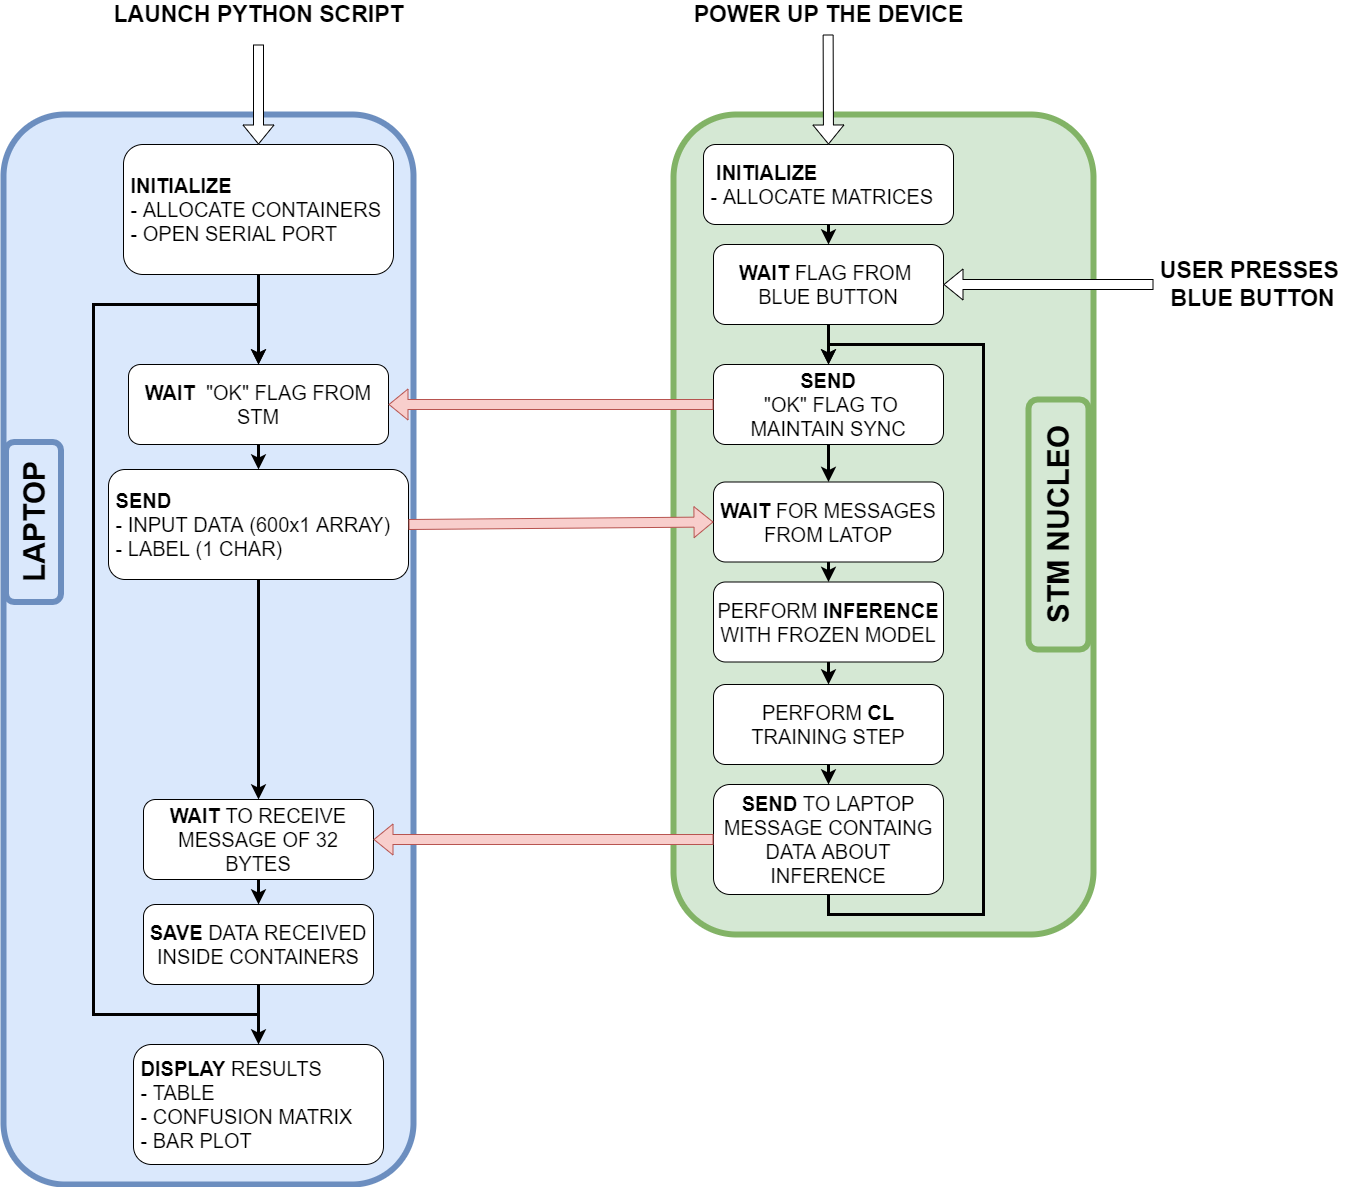
\includegraphics[width=110mm]{Figures/Chapter4/python_nucleo.png} 
    \caption{Block diagram showing the communication between laptop and STM Nucleo.}
    \label{fig:python_stm_diagram}    
\end{figure}



\section{OpenMV setup for image classification}
The application on the OpenMV camera is quite similar. Once the dataset, the model, the last layer, and the system are prepared, everything can be deployed on the MCU. This time, because of the custom board and custom firmware, the toolchain for the deployment of the model is different. Thanks to it, it is possible to include the ML model inside the MCU files and generate from scratch a new firmware that contains the model parameters and structure. This allows to later use built-in-tools for efficient, optimized, and fast inference directly from the MicroPython code. Once the firmware is generated, it can be loaded on the camera MCU through OpenMV IDE.\\
The system developed for the application of CL strategies is basically the same as the one explained in the previous example. Initially, the code allocates the necessary parameters and memory, and later it enters in an infinite while loop. Here, the code continuously waits for a new sample which is then fed to the built-in-tools that perform the frozen model inference. Then, the output is propagated through the CL system. The only major difference in this application is the management of the memory for the matrices. Moreover, problems regarding the allocation of big matrices often block the code. It was decided to not have the entire classification layer inside one single matrix, but rather separate it in smaller sections. This can lead to a small increase of time for the inference, but it is actually required to obtain satisfying reults. \\
Once the code is loaded in the $main.py$ file and the library $TinyOL.py$ is loaded on the MCU, the experiment can be carried out. As before, a Python app was developed for the creation of fast, reliable and repeatable training sessions. Here, the idea is not to send data via USB connection, but display on a screen images from the MNIST dataset while the camera is pointing at it. The USB connection is required anyway because the app needs to maintain sync with the camera and send labels representing the image displayed. This time the app requires the use of Tensorflow (for loading the dataset), OpenCV (for displaying the images on screen) and PySerial (for opening a serial port with the MCU). \\
The app is divided into elemental blocks. At first, the app loads the dataset and extracts from it only the required number of samples. Then, the serial port is opened with the correct characteristics. After that, the app opens two windows, where the first is used for displaying MNIST digits where the camera is be pointed at, while the second is used for displaying in real-time the point of view of the camera. At last, a while loop starts where the communication laptop-MCU is done. At every single step the laptop sends two messages to the camera. The first contains a small 4 char command which defines the state of the OpenMV camera. The size of 4 chars was chosen because it is a fast and unique way for sending a command that is also easy to read from the code point of view. The second message is just the label of the image displayed on the screen. Every time these two messages are received, the camera takes a picture and performs actions depending on its state. The possible states are defined by the user (through the python app) and are: 

\begin{itemize}
	\item $snap$ mode: the camera takes a photo, compresses it and sends it via UART to the laptop. This state is used for understanding where the camera is pointing and if the digit is inside the point of view of the OpenMV. The label received is not used and should be a char containing an $X$.
	\item $elab$ mode: the camera takes a photo, applies a gray scale filter, applies a binarization, compresses the image, and sends it via UART to the laptop. This mode is used for understanding what the camera will see also basic image manipulation is applied. These manipulations are used in the training for transforming the coloured image into a black and white image. Also in this case, the label is discarded and contains just an $X$ char. During this state, the app on the laptop slowly shows all digits from 0 to 9. This permits the user to better point the camera towards the screen.
	\item $trai$ mode: the camera takes a photo, applies inference on the image and later feeds the output to the CL system. No transmission of image is performed towards the laptop because it is easy to un sync the devices. The label this time is received and transformed into a hot one encoded array for the computation of the back propagation.
\end{itemize}

Once the training and the pseudo testing are performed, the app stops showing digit images and the OpenMV camera stores the results inside its SD card. Then, the results are manipulated by a script that transforms the raw data written in the SD card into a table a confusion matrix and bar plots. Figure \ref{fig:python_openmv_diagram} contains a block diagram summarizing the flow of the experiment. 

\begin{figure}[h!]
    \centering
    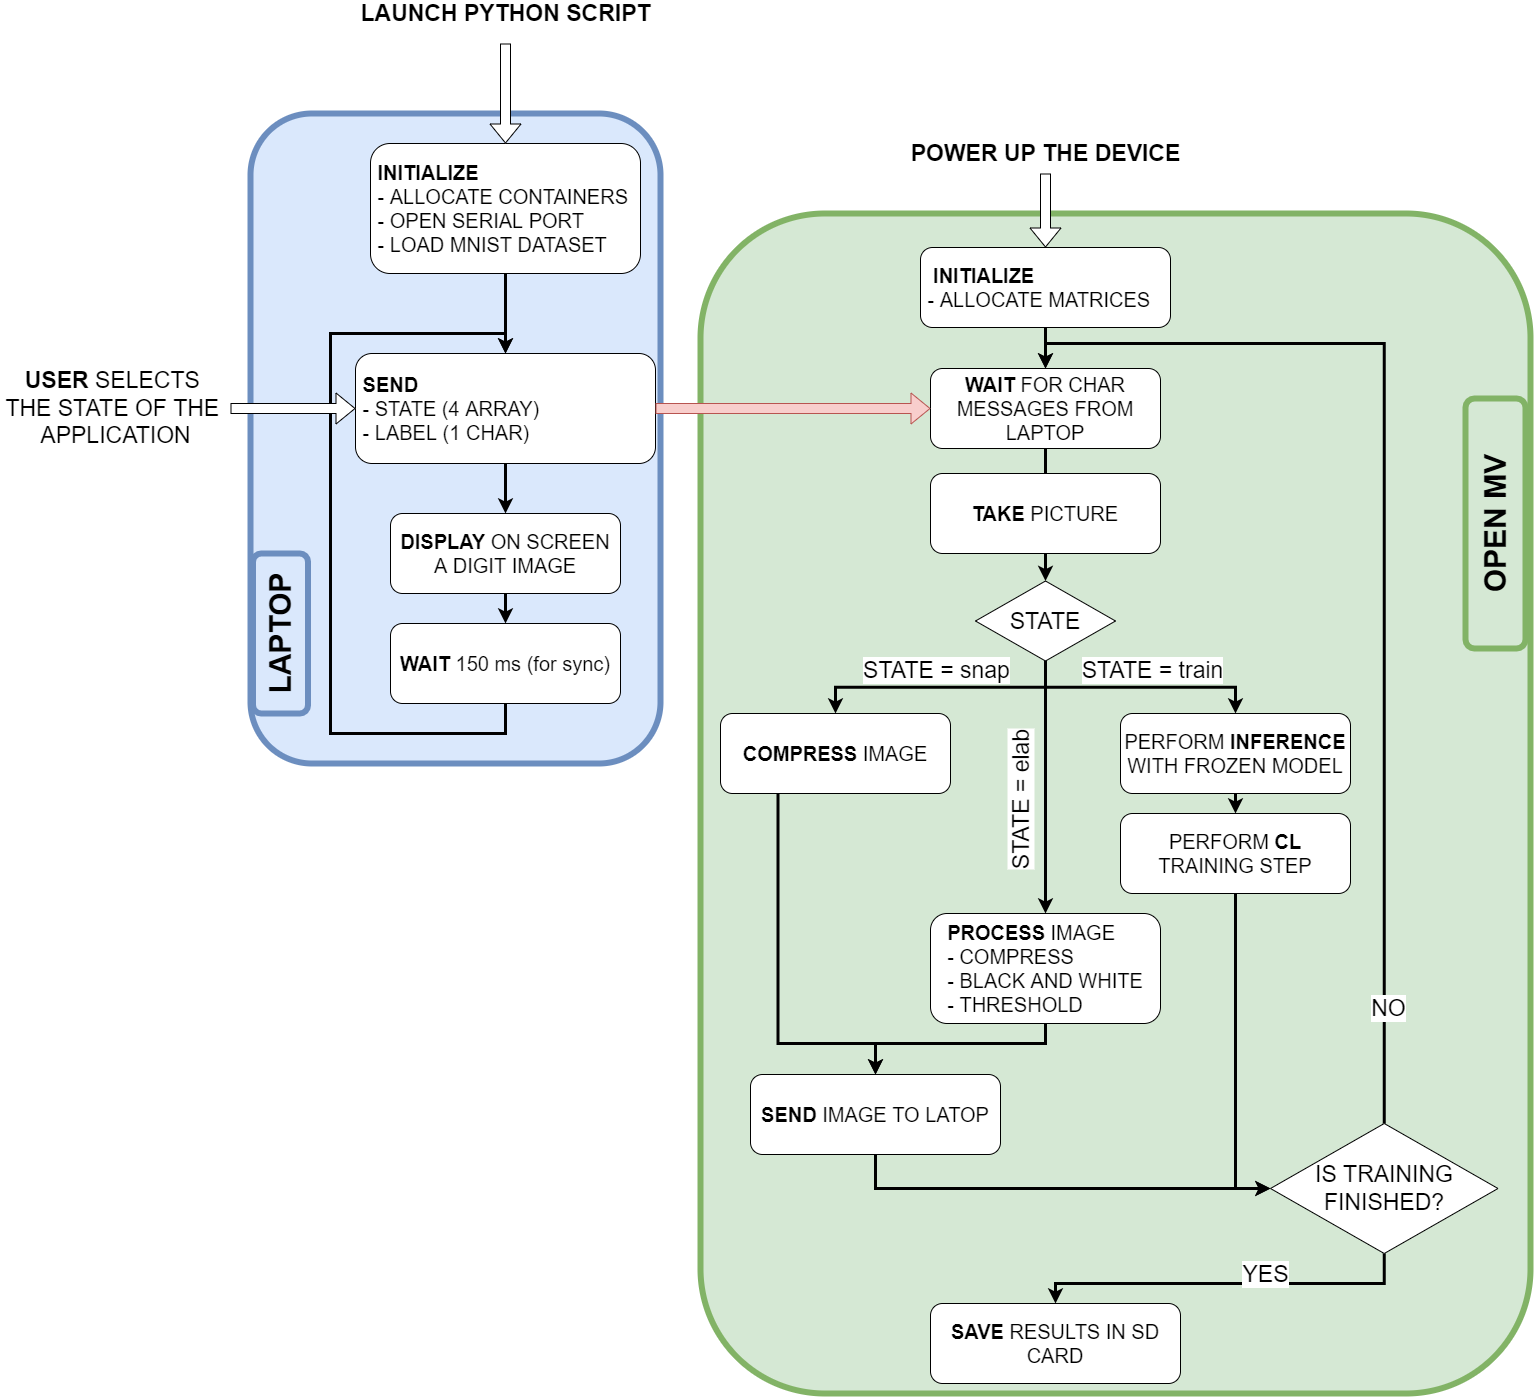
\includegraphics[width=110mm]{Figures/Chapter4/python_openmv.png} 
    \caption{Block diagram showing the communication between laptop and OpenMV camera.}
    \label{fig:python_openmv_diagram}    
\end{figure}

Figure \ref{fig:openmv_training} shows the OpenMV camera pointed to a computer screen in different states. Top right figure shows the camera in $idle$ mode, meaning no stream is received by the laptop. Top left figure represents the camera in $snap$ mode, where compressed images are streamed to the laptop. Bottom left figure contains the camera in $elab$ mode, where compressed and processed images are streamed to the laptop. Bottom right figure shows the camera in $train$ mode, meaning no stream is available and the camera is performing inference and CL training.

\begin{figure}[h!]
    \centering
    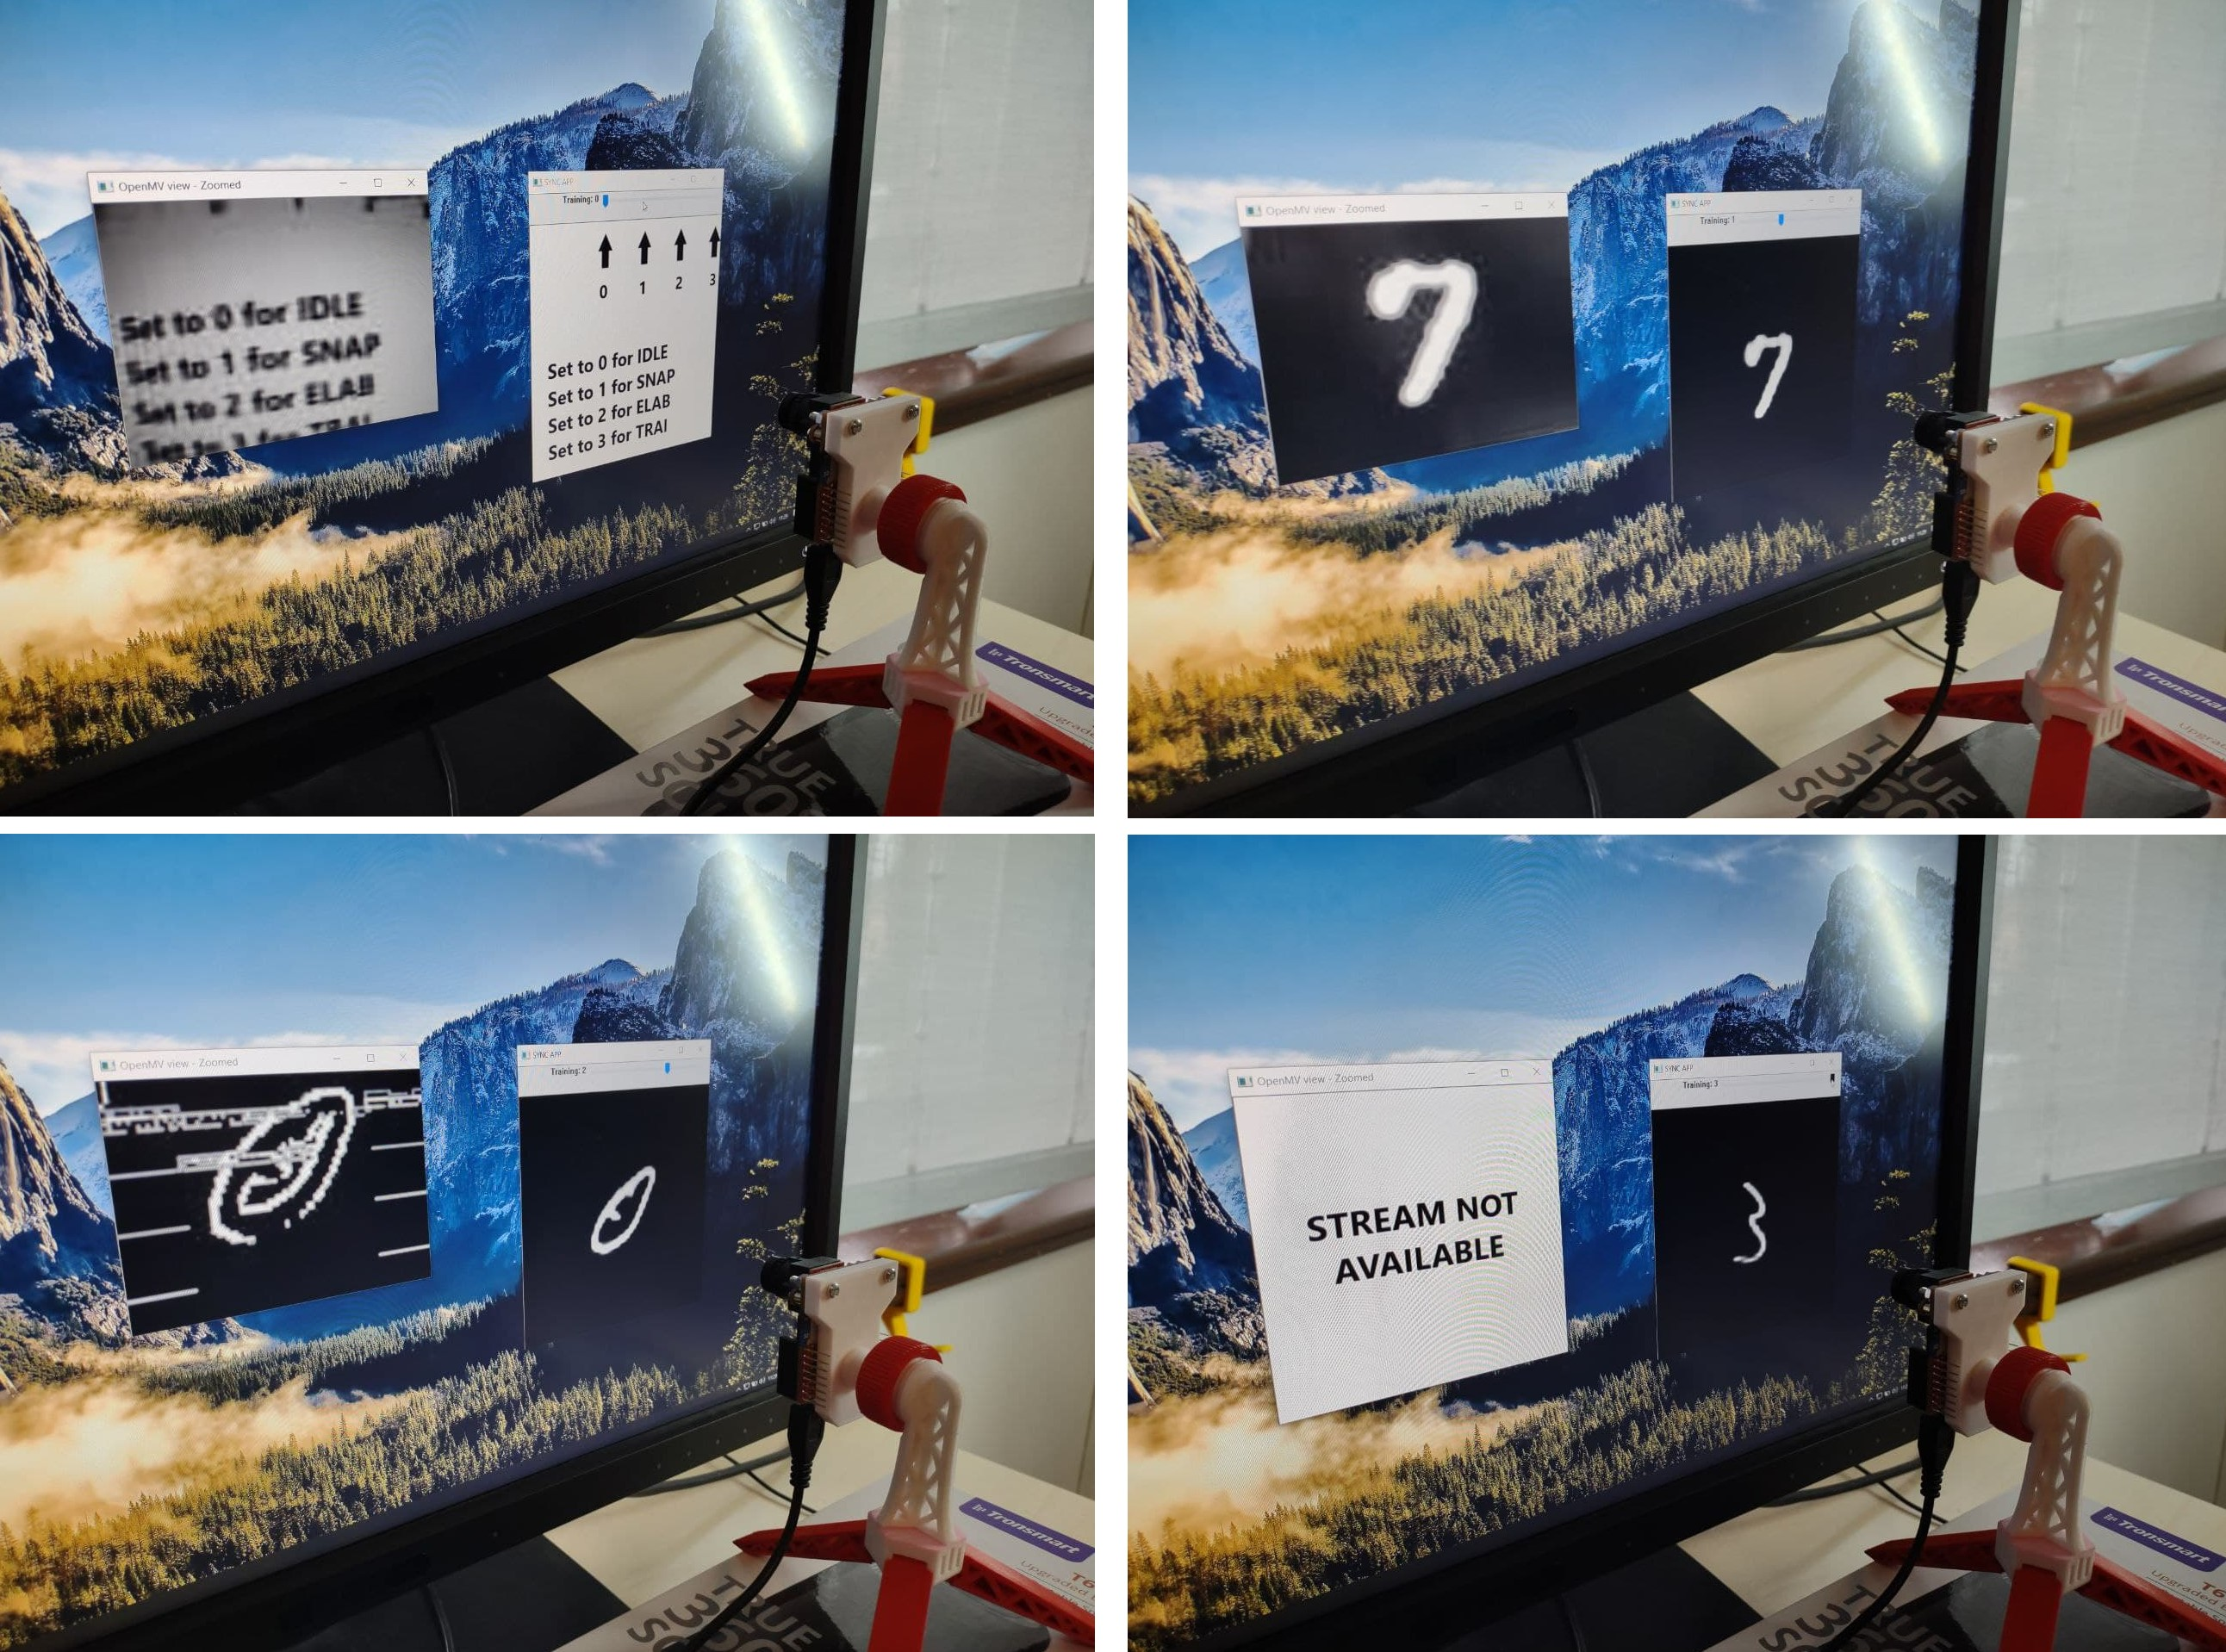
\includegraphics[width=130mm]{Figures/Chapter4/openmv_training.jpg} 
    \caption{OpenMV camera pointing to a screen while in different states of the training. Top left is $idle$ mode, top right is $snap$ mode, bottom left is $elab$ mode, bottom right is $trai$ mode}
    \label{fig:openmv_training}    
\end{figure}

Figures \ref{fig:openmv_pov} shows a better comparison between images taken in the $snap$ and $elab$ mode. As mentioned before, in the $snap$ state the photo is captured, compressed, and sent. In $elab$ mode the image is captured, gray scaled, binarized with threshold, compressed, and sent.

\begin{figure}[h!]
    \centering
    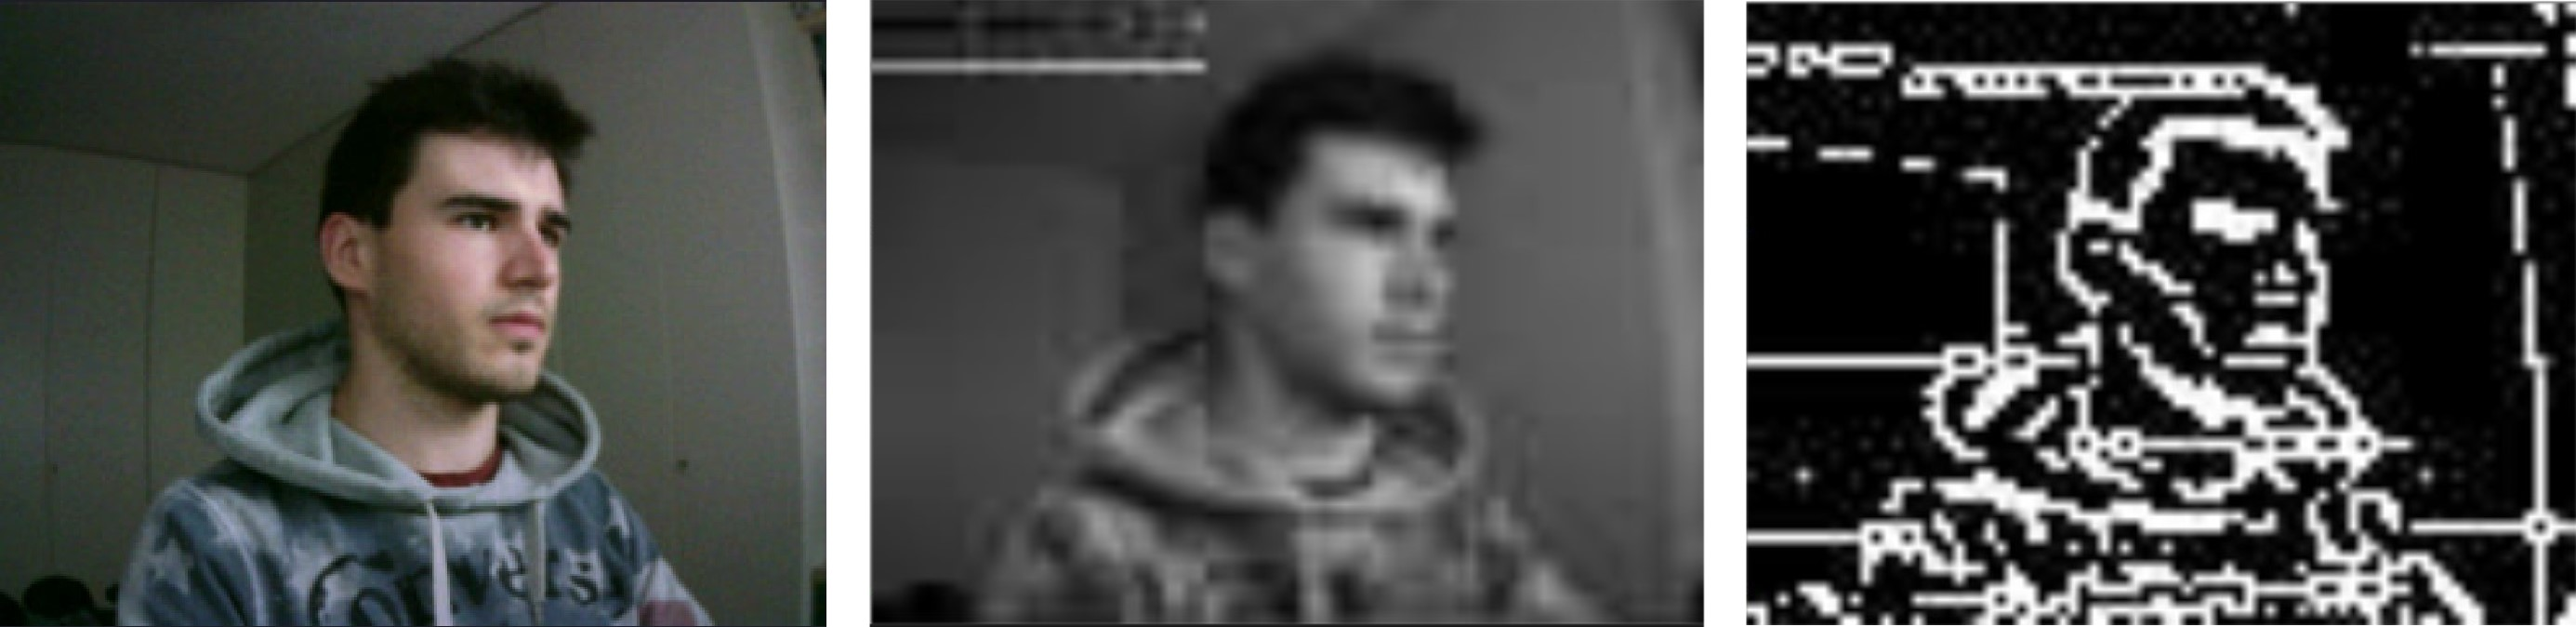
\includegraphics[width=140mm]{Figures/Chapter4/openmv_pov.jpg} 
    \caption{Point of view of the OpenMV camera. On the left the original image taken with no compression and no elaboration, in the center an image taken in $snap$ mode, on the right an image taken in $elab$ mode.}
    \label{fig:openmv_pov}    
\end{figure}


\chapter{Experimental results} 

\section{Experiment A: Gesture recognition}

\section{Experiment B: Image classification}

This section contains and explains the results obtained from the test performed. Initially a description about the comparison between simulation and real application is performed with the aim of understanding if the training on the nucleo evolves as the simulation on the laptop. Then the results obtained from the application from the Nucleo are discussed and finally the results from the OpenMV application are described.\\
To understand if the Nucleo STM32 F401-RE is able to perform a real-time ML training a study concerning the history of its parameters is done. The idea is to record the variation of the most important parameters from the OL layer at every training step and then compare its evolution to the same parameter evolutioin but recorded from the simulation carried out on the laptop. The parameters of interest are the biases of the OL layer, the predictions obtained from Softmax, the output of the frozen model, 10 weights picked randomically from the weight matrix. The evolution of the parameters is then displayed in a plot with the aim of observing how and if the history recorded from the laptop differs from the history recorded from the MCU. This is done qualitatively simply by looking at superimposition of the two lines. Figure \ref{fig:comparison_frozen} shows one example of comparison for the frozen model outpus, figure \ref{fig:comparison_bias} shows the comparison of the bias evolution, figure \ref{fig:comparison_weights} shows the comparison of the weights evolution, figure \ref{fig:comparison_softmax} shows the difference of the predictions obtained from Softmax.
%
\begin{figure}[h!]
    \centering
    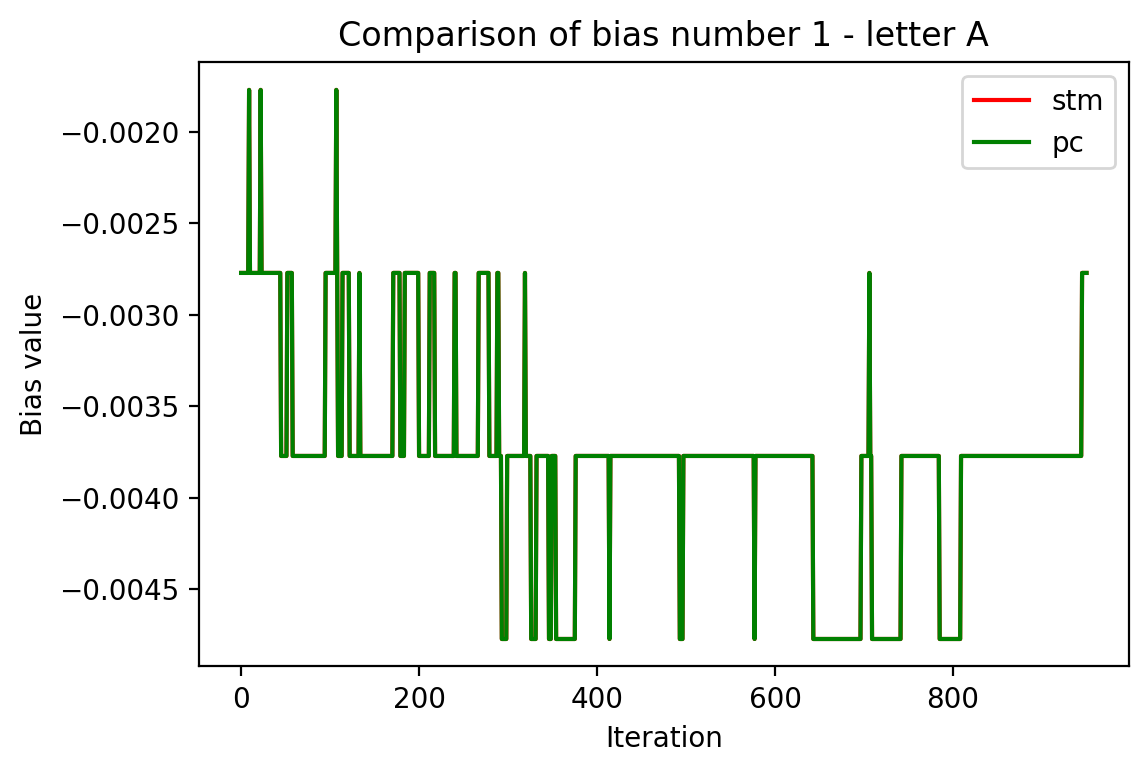
\includegraphics[width=100mm]{Figures/Chapter5/bias_example.png} 
    \caption{PLACEHOLDER}
    \label{fig:comparison_bias}    
\end{figure}
%
%
\begin{figure}[h!]
    \centering
    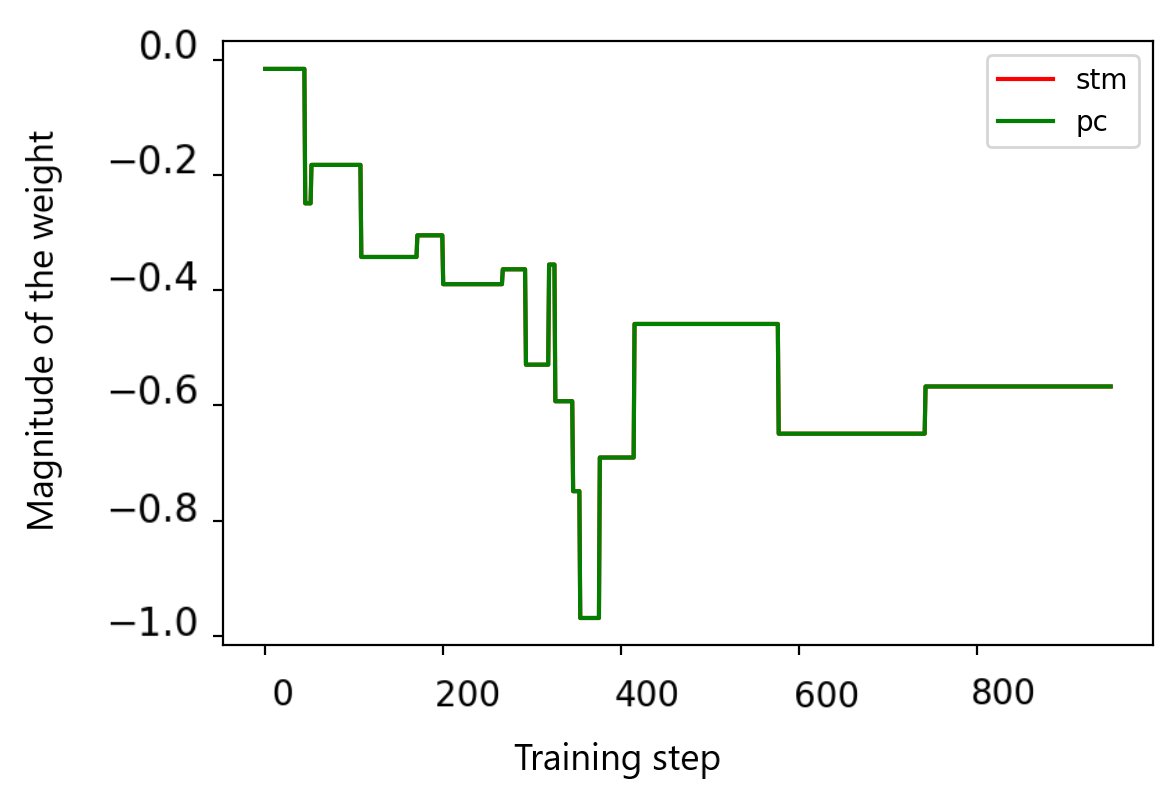
\includegraphics[width=100mm]{Figures/Chapter5/weight_example.png} 
    \caption{PLACEHOLDER}
    \label{fig:comparison_weights}    
\end{figure}
%
%
\begin{figure}[h!]
    \centering
    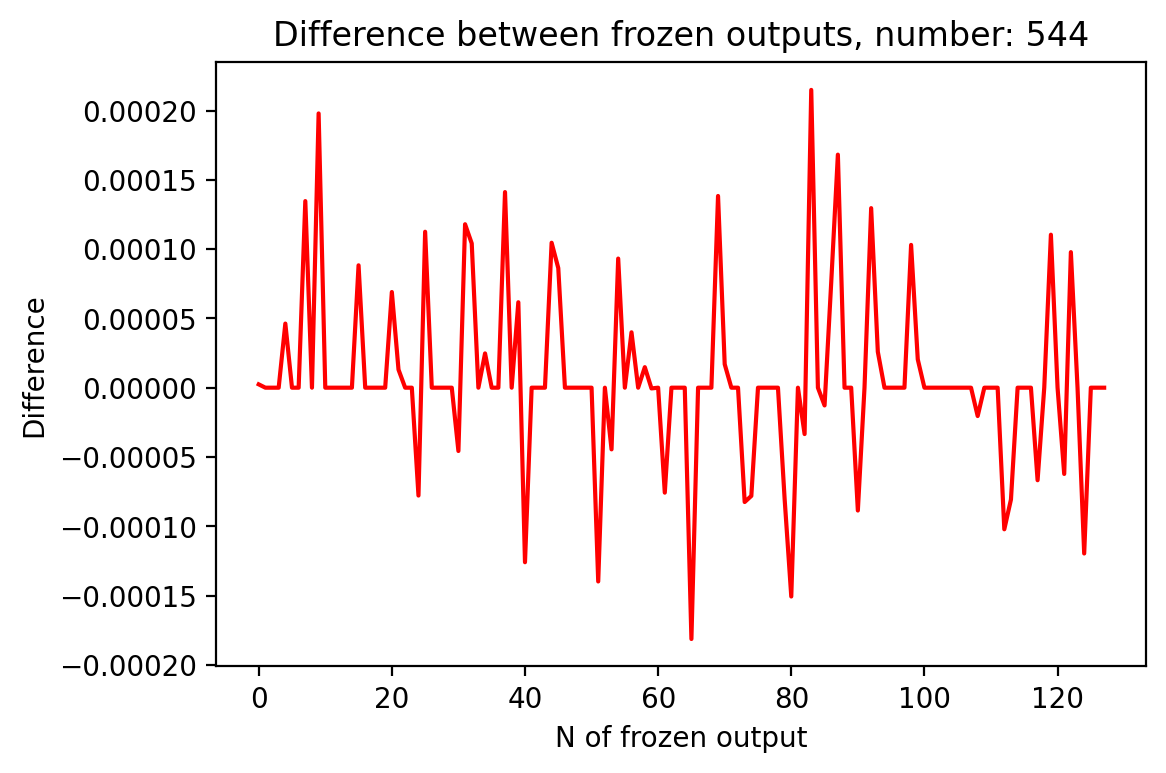
\includegraphics[width=100mm]{Figures/Chapter5/frozen_example.png} 
    \caption{PLACEHOLDER}
    \label{fig:comparison_frozen}    
\end{figure}
%
%
\begin{figure}[h!]
    \centering
    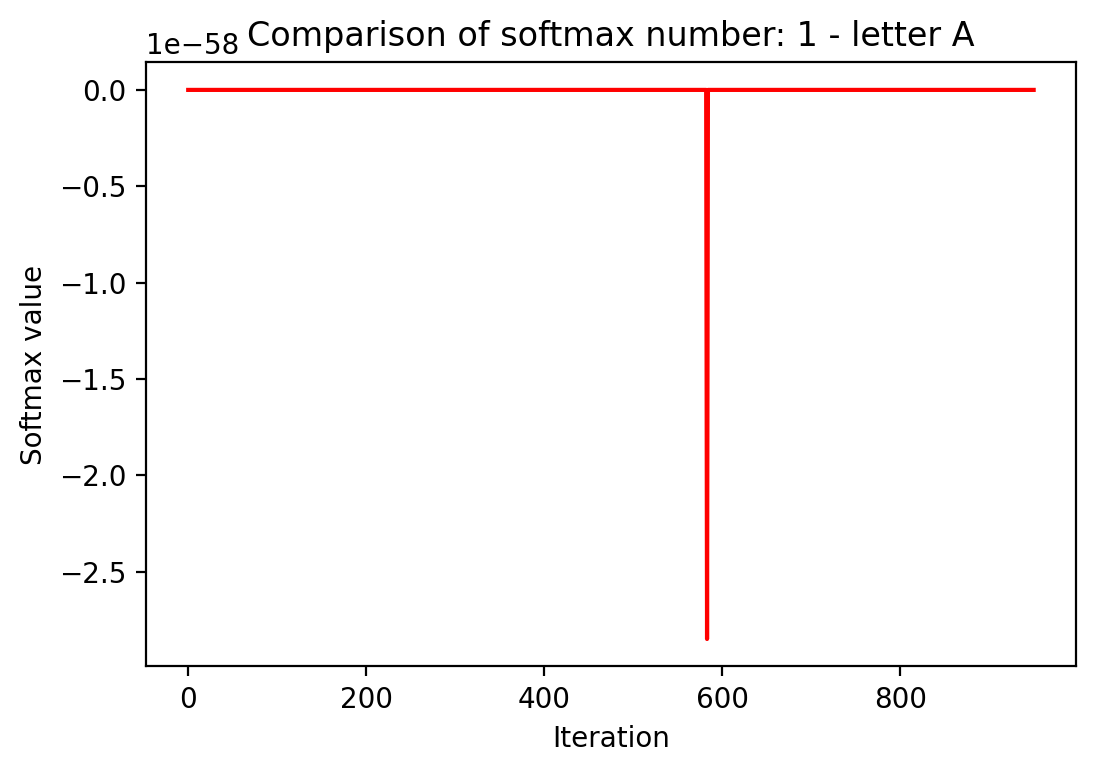
\includegraphics[width=100mm]{Figures/Chapter5/softmax_example.png} 
    \caption{PLACEHOLDER}
    \label{fig:comparison_softmax}    
\end{figure}
%
The plots displayed above are examples of the evolution performed, but they are rappresentative of the behaviour of all parameters. It's clear from the results how the two applications are very close, differencing from each other by just a small magnitude and for very few training step. Only one difference can be noted in figure x, where the dofference of the softmax prediction is dofferent from zero but still very little. This error in fact doesn't introduce any problem in the evolution since in the following steps the error goes back to 0. \\
One of the main concerns was about the feature extraction performed by the frozen model. Because of the limited resources of the MCU usually models are compressed to be later loaded on the device. In this case no pruning or quantization have been applied, so the frozen model loaded on the MCU and laptop are exactly the same. The concern regards how the prediction is carried out by the X-CUBE-AI tool on the MCU compared with Tensorflow on the laptop. Figure \ref{fig:comparison_max} contains two examples of comparison of frozen model outputs. The x axis contains the iterator representing the i-th difference computed between the i-th value from the Tensorflow and STM output from the frozen model. On the left the difference that contains the biggest error is displayed, while on the right is displayed the sample that contains the second biggest error. It's clear how the plot on the left is not a correct representation of the MCU behaviour since it has a magnitude far too high when compared to the second biggest error.
%
\begin{figure}[h!]
    \centering
    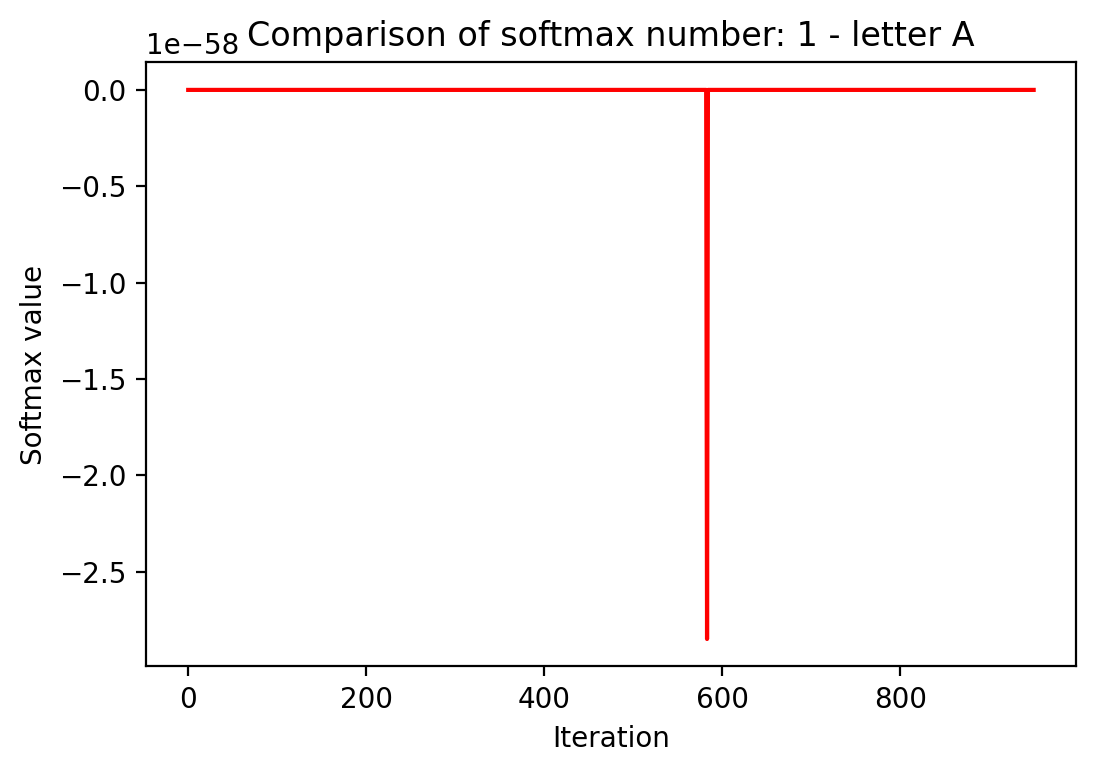
\includegraphics[width=100mm]{Figures/Chapter5/comparison_difference.png} 
    \caption{PLACEHOLDER}
    \label{fig:comparison_max}    
\end{figure}
%
Thanks to this study it is possible to conclude that a training performed on such a small device is actually possible and in terms of accuracy and precision it is as reliable as a training performed on a powerful device. Because of these plots it is then possible to conclude that the evolution of the model on the MCU is reliable and correct. A model trained on such device is subject to the same exact evolution that would affect the model in the case the training were to be carried on a laptop. From this point on all the experiment and results are obtained from MCUs.
\bigskip

Speaking about the gesture recognition experiment once the training have been carried out it's possible to display the accuracy of every single algorithm for every single class. As mentioned in section REFERENCE SECTION the testing is performed on the last 20 \% of the dataset, so on a total of XXX samples. The bar plots containing the accuracies from every strategy together with their confusion matrices are displayed in Figures \ref{fig:letter_res_OL} \ref{fig:letter_res_OL_batch} \ref{fig:letter_res_OL_v2} \ref{fig:letter_res_OL_v2_batch} \ref{fig:letter_res_LWF} \ref{fig:letter_res_LWF_batch} \ref{fig:letter_res_CWR}.  
%
\begin{figure}[h!]
    \centering
    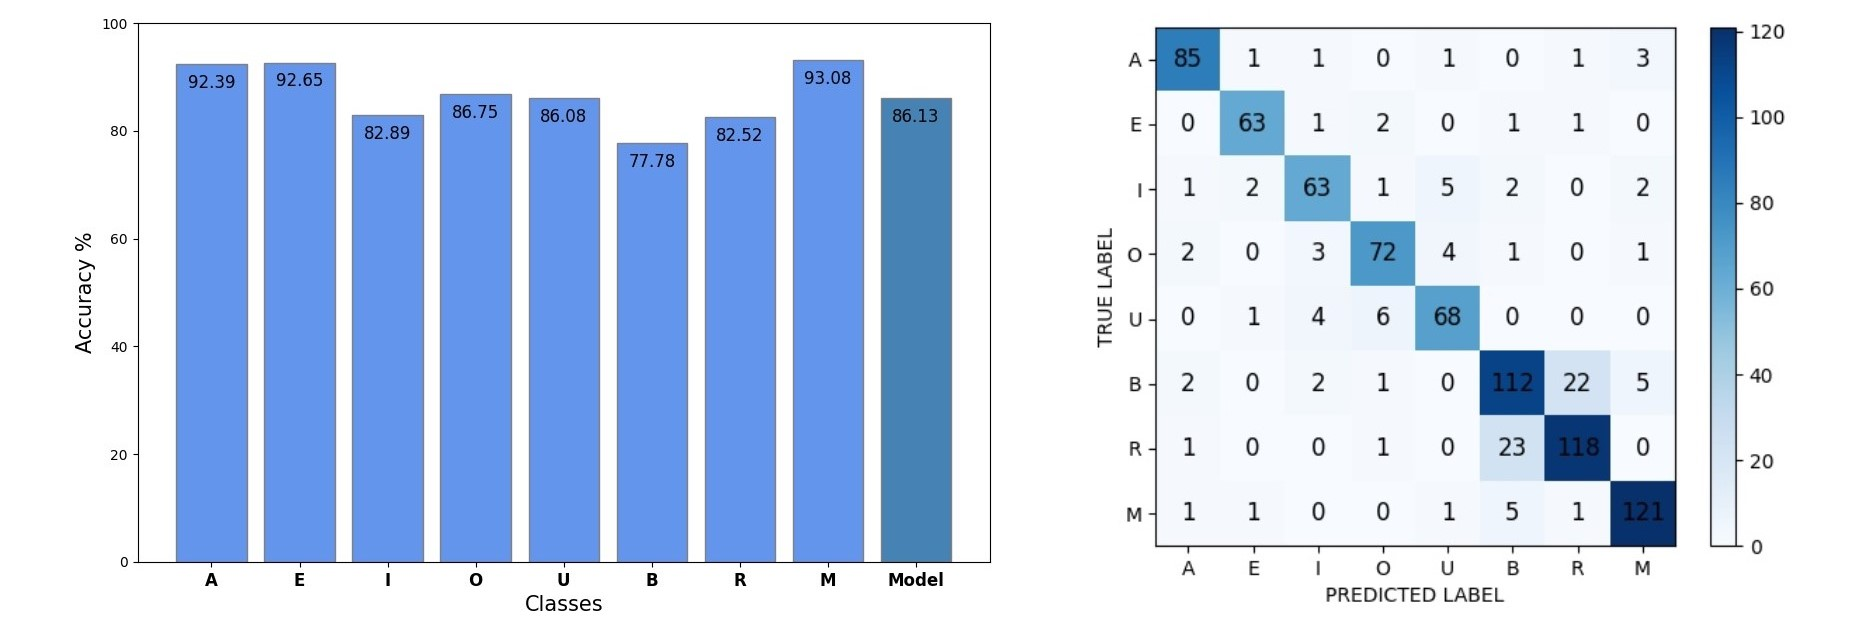
\includegraphics[width=100mm]{Figures/Chapter5/STM_barPlot_OL.jpg} 
    \caption{PLACEHOLDER}
    \label{fig:letter_res_OL}    
\end{figure}
%
%
\begin{figure}[h!]
    \centering
    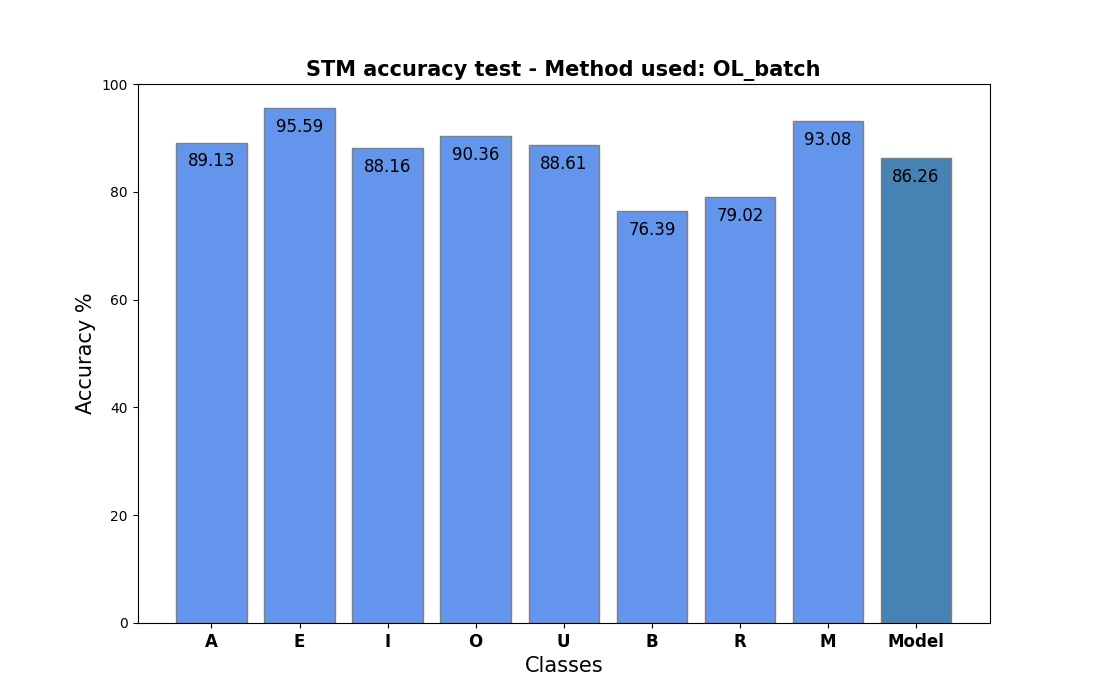
\includegraphics[width=100mm]{Figures/Chapter5/STM_barPlot_OL_batch.jpg} 
    \caption{PLACEHOLDER}
    \label{fig:letter_res_OL_batch}    
\end{figure}
%
%
\begin{figure}[h!]
    \centering
    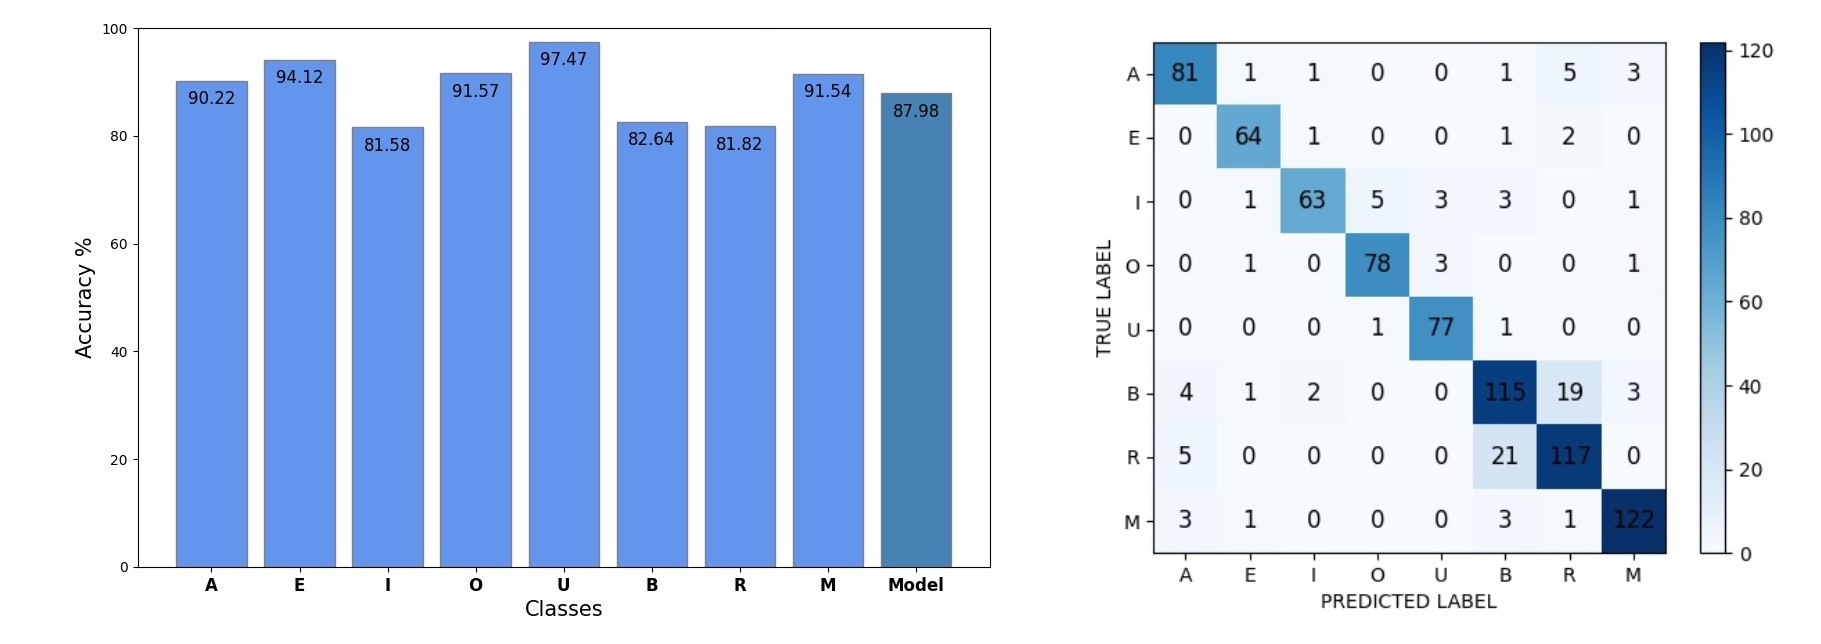
\includegraphics[width=100mm]{Figures/Chapter5/STM_barPlot_OL_V2.jpg} 
    \caption{PLACEHOLDER}
    \label{fig:letter_res_OL_v2}    
\end{figure}
%
%
\begin{figure}[h!]
    \centering
    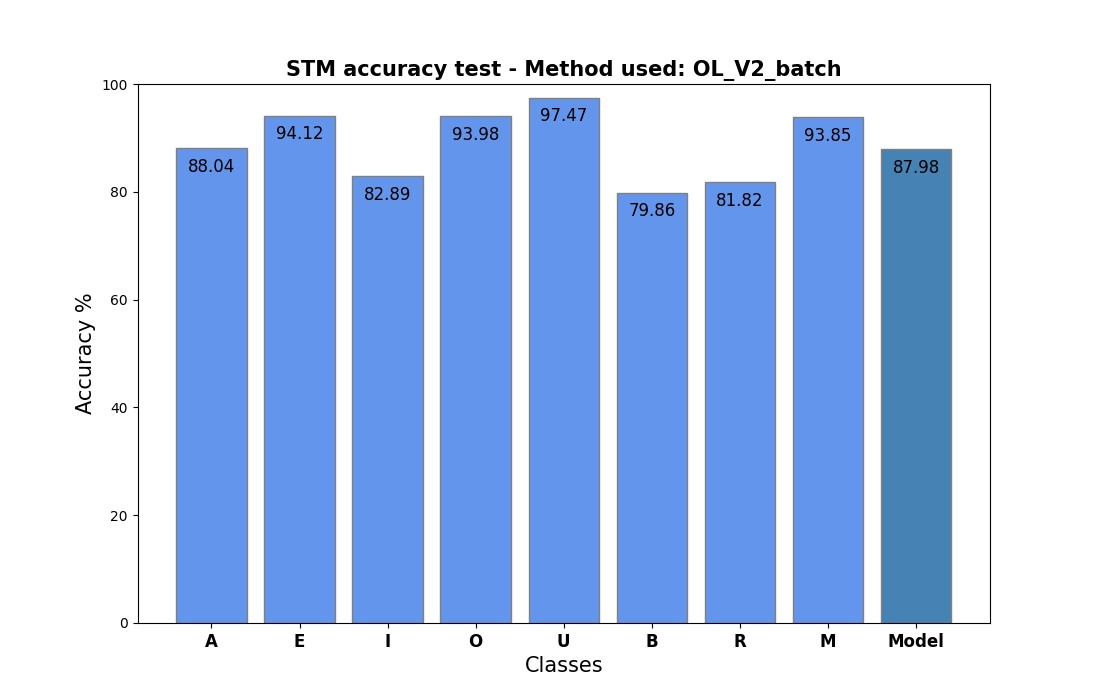
\includegraphics[width=100mm]{Figures/Chapter5/STM_barPlot_OL_V2_batch.jpg} 
    \caption{PLACEHOLDER}
    \label{fig:letter_res_OL_v2_batch}    
\end{figure}
%
%
\begin{figure}[h!]
    \centering
    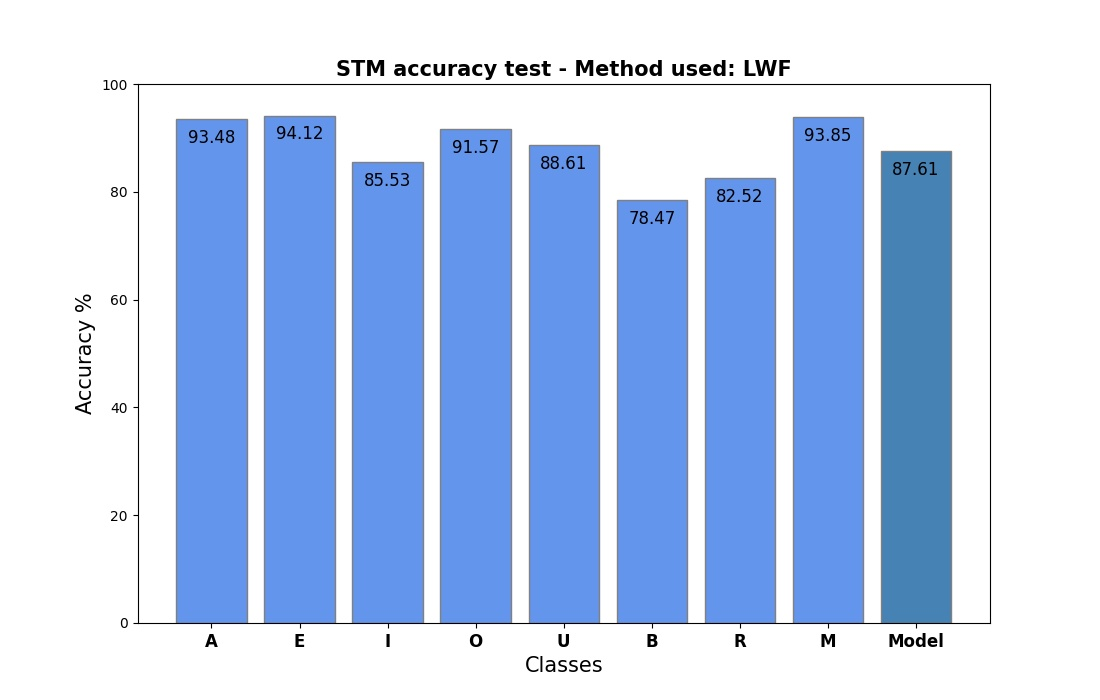
\includegraphics[width=100mm]{Figures/Chapter5/STM_barPlot_LWF.jpg} 
    \caption{PLACEHOLDER}
    \label{fig:letter_res_LWF}    
\end{figure}
%
%
\begin{figure}[h!]
    \centering
    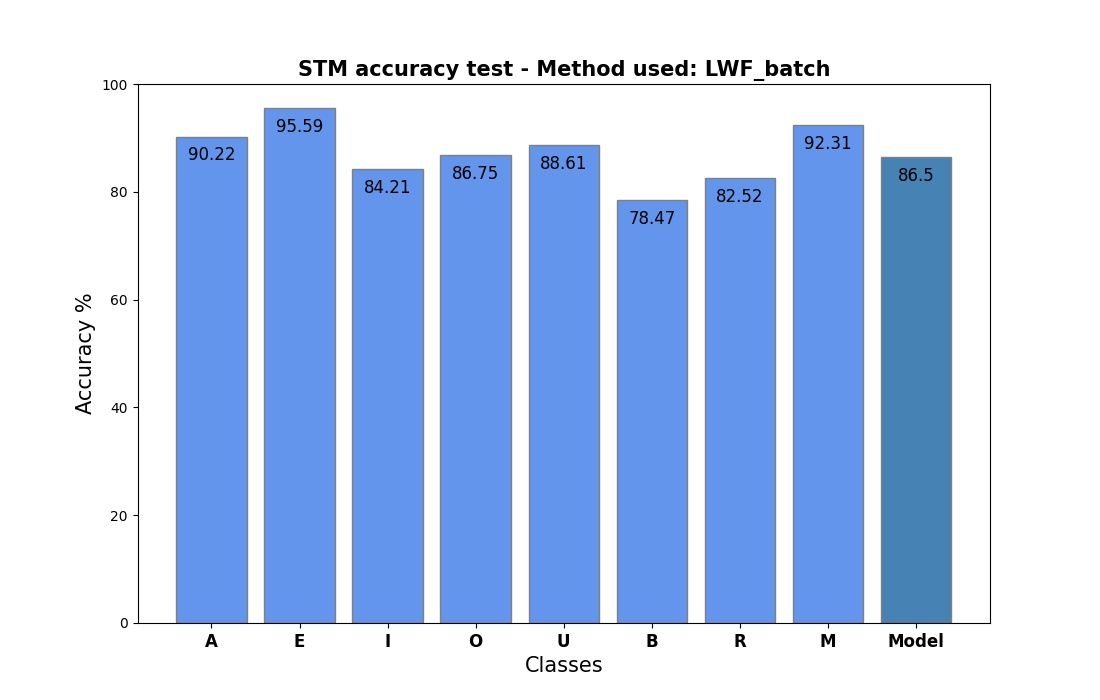
\includegraphics[width=100mm]{Figures/Chapter5/STM_barPlot_LWF_batch.jpg} 
    \caption{PLACEHOLDER}
    \label{fig:letter_res_LWF_batch}    
\end{figure}
%
%
\begin{figure}[h!]
    \centering
    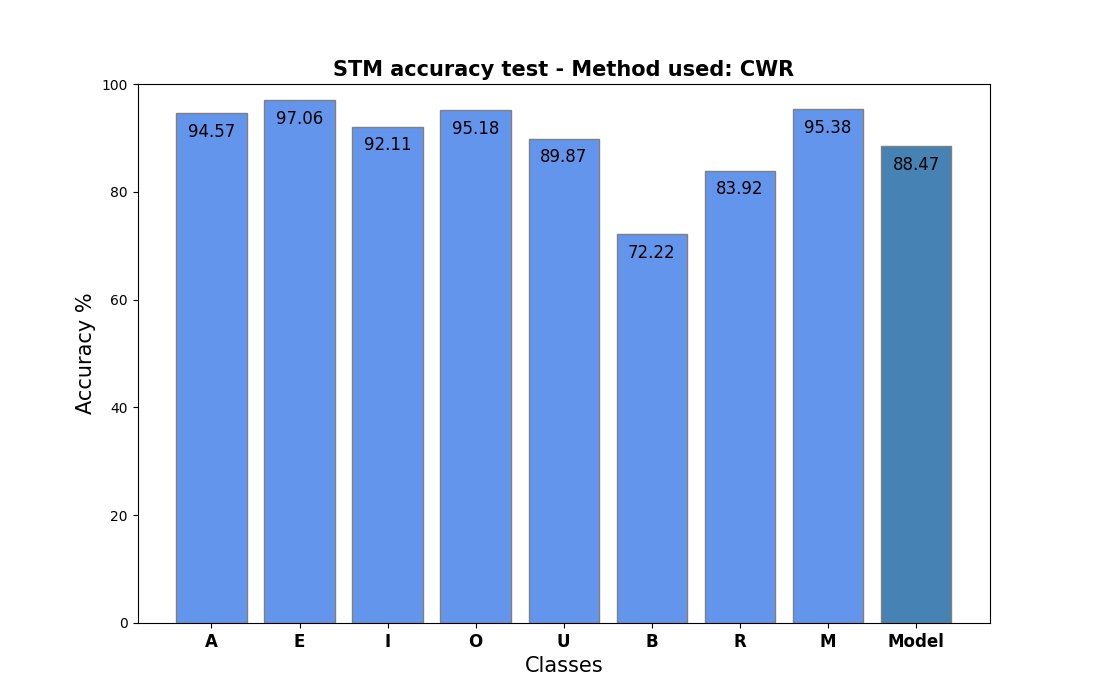
\includegraphics[width=100mm]{Figures/Chapter5/STM_barPlot_CWR.jpg} 
    \caption{PLACEHOLDER}
    \label{fig:letter_res_CWR}    
\end{figure}
%
From these plots it is clear how all methods are quite good in digesting new classes and completely fuse them in the classification layer. No method in fact shows a bad learning on a specific class exept for the letter B that in all methods sees a lower accuracy when compared to others. It' easy to see from the cofusion matrix that the letter is not learned in a wrong way but rather the letter is easily confused with the letter R. Most probably this is because the path that has been followed when the dataset has beenc reated differs for just the leg of letter R. \\
Table x and table x contain other important results from the experiment. 
%
\begin{table}[]
\begin{center}
\begin{tabular}{l|cccc}
                     & \multicolumn{1}{c|}{\textbf{Accuracy \%}} & \multicolumn{1}{c|}{\textbf{\begin{tabular}[c]{@{}c@{}}Average time\\ inference frozen\\  model in ms\end{tabular}}} & \multicolumn{1}{c|}{\textbf{\begin{tabular}[c]{@{}c@{}}Average time \\ inference OL\\ layer in ms\end{tabular}}} & \multicolumn{1}{c|}{\textbf{\begin{tabular}[c]{@{}c@{}}Maximum allocated \\ RAM in kB\end{tabular}}} \\ \hline
\textbf{OL}          & 86.13                                     & 10.65                                                                                                                & 0.99                                                                                                             & 26.1                                                                                                 \\ \cline{1-1}
\textbf{OL batch}    & 86.26                                     & 10.65                                                                                                                & 1.54                                                                                                             & 29.8                                                                                                 \\ \cline{1-1}
\textbf{OL V2}       & 87.98                                     & 10.65                                                                                                                & 1.03                                                                                                             & 26.1                                                                                                 \\ \cline{1-1}
\textbf{OL V2 batch} & 87.98                                     & 10.65                                                                                                                & 1.11                                                                                                             & 29.8                                                                                                 \\ \cline{1-1}
\textbf{LWF}         & 87.61                                     & 10.65                                                                                                                & 3.45                                                                                                             & 29.9                                                                                                 \\ \cline{1-1}
\textbf{LWF batch}   & 86.5                                      & 10.65                                                                                                                & 3.26                                                                                                             & 29.9                                                                                                 \\ \cline{1-1}
\textbf{CWR}         & 88.47                                     & 10.65                                                                                                                & 2.11                                                                                                             & 29.9                                                                                                 \\ \cline{1-1}
\textbf{MY ALG}      & 86.87                                     & 10.65                                                                                                                & 3.54                                                                                                             & 29.9                                                                                                 \\ \cline{1-1}
\end{tabular}
\end{center}
\end{table}
%
\begin{table}[]
\begin{tabular}{cc|cccccccccc}
\multicolumn{1}{c|}{\multirow{2}{*}{Algorithm}} & \multirow{2}{*}{Parameter} & \multicolumn{8}{c|}{Class}                                                                                                                                                                            & \multicolumn{1}{c|}{\multirow{2}{*}{\begin{tabular}[c]{@{}c@{}}batch\\ size\end{tabular}}} & \multirow{2}{*}{\begin{tabular}[c]{@{}c@{}}learning\\ rate\end{tabular}} \\
\multicolumn{1}{c|}{}                           &                            & \multicolumn{1}{c|}{A} & \multicolumn{1}{c|}{E} & \multicolumn{1}{c|}{I} & \multicolumn{1}{c|}{O} & \multicolumn{1}{c|}{U} & \multicolumn{1}{c|}{B} & \multicolumn{1}{c|}{R} & \multicolumn{1}{c|}{M} & \multicolumn{1}{c|}{}                                                                      &                                                                          \\ \hline
\multirow{3}{*}{OL}                             & Accuracy                   & 0.92                   & 0.93                   & 0.83                   & 0.87                   & 0.86                   & 0.78                   & 0.83                   & 0.93                   & \multirow{3}{*}{16}                                                                        & \multirow{3}{*}{16}                                                      \\ \cline{2-2}
                                                & Precision                  & 0.92                   & 0.93                   & 0.85                   & 0.87                   & 0.86                   & 0.78                   & 0.83                   & 0.92                   &                                                                                            &                                                                          \\ \cline{2-2}
                                                & F1 score                   & 0.92                   & 0.93                   & 0.84                   & 0.87                   & 0.86                   & 0.78                   & 0.83                   & 0.92                   &                                                                                            &                                                                          \\ \cline{1-2}
\multirow{3}{*}{OL batch}                       & Accuracy                   & 0.89                   & 0.96                   & 0.88                   & 0.90                   & 0.89                   & 0.76                   & 0.79                   & 0.93                   & \multirow{3}{*}{16}                                                                        & \multirow{3}{*}{16}                                                      \\ \cline{2-2}
                                                & Precision                  & 0.93                   & 0.97                   & 0.89                   & 0.91                   & 0.85                   & 0.75                   & 0.78                   & 0.93                   &                                                                                            &                                                                          \\ \cline{2-2}
                                                & F1 score                   & 0.91                   & 0.96                   & 0.88                   & 0.90                   & 0.87                   & 0.75                   & 0.78                   & 0.93                   &                                                                                            &                                                                          \\ \cline{1-2}
\end{tabular}
\end{table}

In table x the overall accuracy of the model with specific strategies is displayed. From here it's clear how the algorithm CWR performs the best with an accuracy of xx \%. All methods perform quite good with the lowest accuracy being xx \& from the method OL, which is just a drop of xx \% with respect to the accuracy obtained from the training of the frozen model performed with Tensorflow. Speaking about the time required for a training step the total time can be split in two portions. The first concerns the inference obtainde by the frozen model, which is of course constant for all strategies and takes 10.65 ms. The other part of the training step time is the time taken by the OL layer which contains the time required for the inference of the OL layer and the following computation of the back propagation and update of the layer's weights. From the table is clear how the faster methods are TinyOL and TinyOL v2, which are the only methods that do require only one OL layer, thus reducing the amount of computations require. On the other hand the slowest methods are LWF, LWF batch and MY ALG, which all require a double inference from the two classification layer. The time is in fact more than double the time required by all the other strategies. The last column concerns the amount of RAM allocated by the strategies. This value shows that the TinyOL and TinyOL v2 are the lightest methods since they require only the allocation of 1 weights matrix and 1 bias array. All the other methods require a very similar amount of RAM since they all work with double memories. A little difference of just 100 bytes is due to the allocation of some additional values particular for some strategies.  \\
Another important study that has been carried out is the study of variation of the accuracy while changing the batch size. This study was of particular interest thanks to \ref{}, a blog post that studies in detail the impact that the batch size has on a ML training. The results are show in figure \ref{fig:batch_size_letter}. Here is clear how the only methods that drop their accuracy quite a bit are TinyOL and TinyOL v2, while all the other are able to mantain their accuracy quite constant.
%
\begin{figure}[h!]
    \centering
    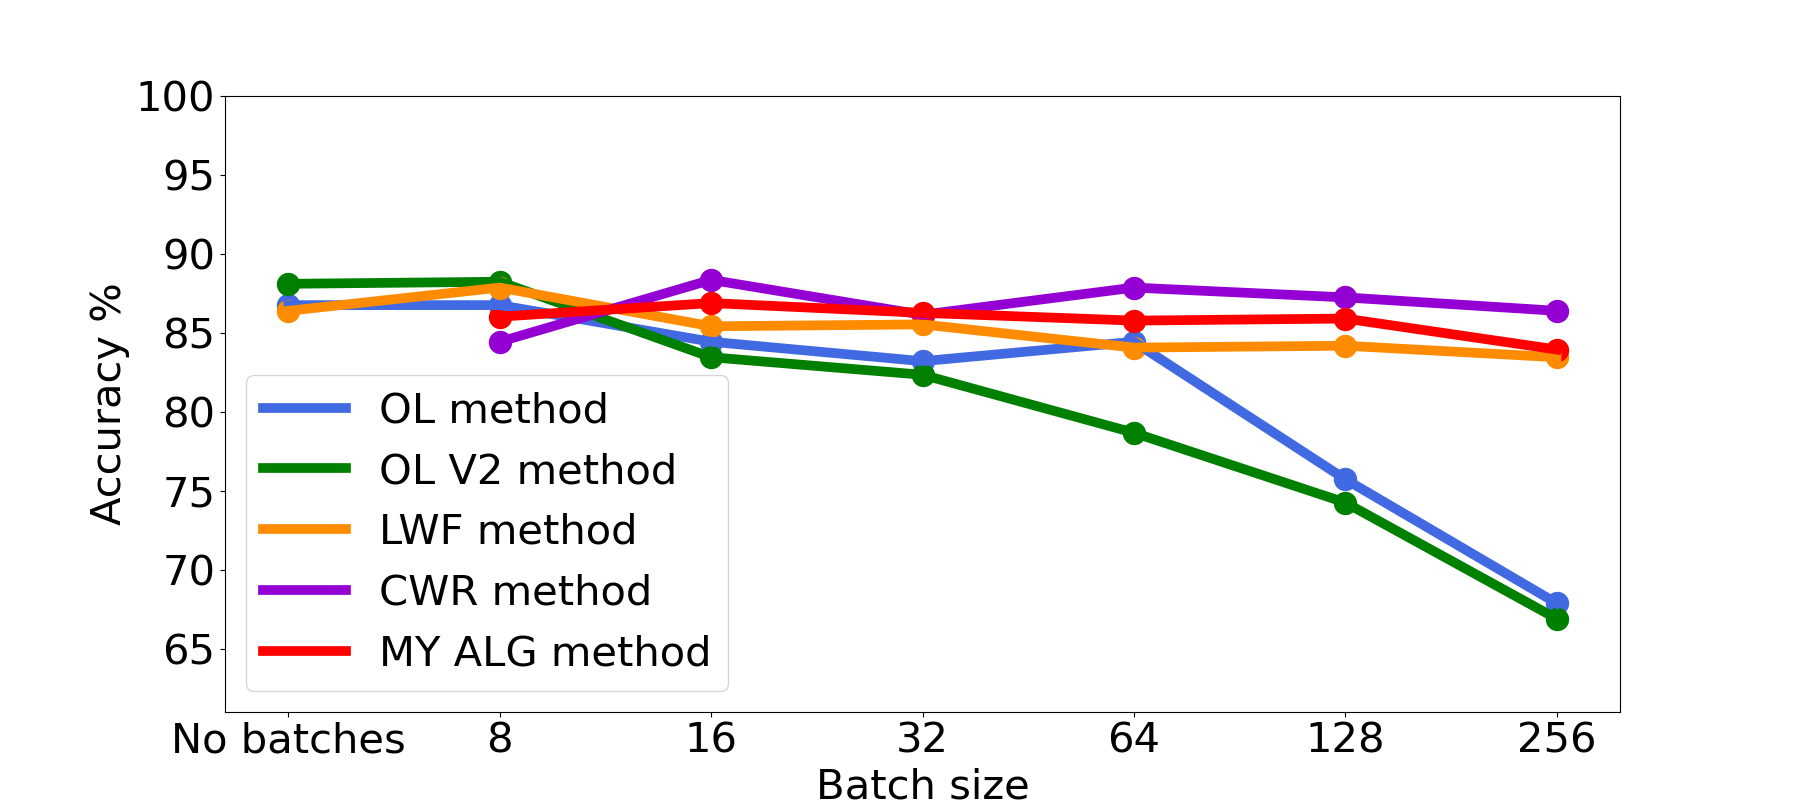
\includegraphics[width=100mm]{Figures/Chapter5/batch_size_letters.png} 
    \caption{PLACEHOLDER}
    \label{fig:batch_size_letter}    
\end{figure}
%

\chapter{Conclusion}
% 1 pag e mezza. Un carrellata di contesto, motivazioni, cosa ho fatto vedere. Per mezza pag poi descrivere future works da cui posso far partire il mio lavoro. 
% Importante scrivere bene intro e conclusioni perchè sono le parti che la commissione legge durante la presentazione oThis thesis  prima. 
This thesis introduces the concept of continual learning on microcontrollers for the application of self-learning ML models on smart sensors. In TinyML applications it is common to deploy devices in scenarios that are subject to context drift. This can make the models degrade in accuracy quite quickly, which leads to unusable and not reliable devices. In these cases it is necessary to apply continual learning strategies. These help the models by introducing flexibility and adaptability characteristics to the model that are now able to follow the context drift.\\
In this thesis a total of 4 different CL strategies have been implemented. Four of these are state-of-the-art methods while one is a simple modification of of them. Additionally small variations of the same methods were implemented to allow for trainings over batches of data. The algorithms have been developed in a framework initially tested on a powerful device and later ported on two microcontrollers. The MCUs use built in tools for the application of ML inference paired with the framework for the integration of CL capabilities. Both microcontrollers perform classification on the data which are recorded from their relative sensors (an accelerometer and a camera).\\
In application A, CL was applied for gesture recognition. An ML model was initially trained on a powerful device for the elaboration of accelerometer data representing letters written in the air. Initially the model was trained for the classification of only vowels, later the CL framework is used for recognizing, including and fine tuning three new classes representing three consonants (B,R,M). 
In application B, the system is used for classification of images. A model is initially trained for the recognition of the first 6 digits (from 0 to 5) from the MNIST dataset. Later the model is equipped with the CL framework that permits the MCU to learn 4 new classes (digits from 6 to 9).\\
Both applications have been implemented in supervised settings. For the gesture application the data and the label were provided via USB, while for the image classification case, the digits are displayed on a screen and the label is provided via USB cable.
All algorithms in both applications proved to be effective in NIC scenarios (new instances and classes). After one training session each method showed that all classes were incorporated correctly in the model. No method was able to outperform the original version of the model (the one trained on the powerful device), but the accuracy drops are always acceptable. For the gesture recognition case the maximum drop is of $10.7 \%$, while for the image classification case the maximum drop is of $6.3 \%$. The degradation of performances is to be considered a necessary trade-off required for the implementation of flexible models that can adapt quickly to changes of context and appearance of new classes.\\

A possible future implementation of the work done up to now is the implementation of the framework for unsupervised settings. One of the main drawback of this study is the inability of the MCUs to be completely autonomous. This is due to the supervised setting in which the trainings are performed. The devices require one ground truth label for each sample provided, which in these tests is provided from the dataset itself. Such an application cannot be used in real-life application because of the lack of a continuous stream of labelled data.\\
Another important implementation is the improvement of compatible layers. The applications seen here are focused on the use of CL for classifications. These models are characterized by the presence of $Softmax$ as activation function on the last layer, where CL is applied. This is an important aspect because the activation function defines the rule to be used for the back propagation. By expanding the compatibility of the framework to other types of layers, the framework could be deployed in many different applications and on different model.\\
One last possible future work comprehends more tests. In this study all test were performed with dataset containing balanced and shuffled data. Scenarios like these damp the phenomenon of catastrophic forgetting because the randomization of the samples makes it possible for the model to continuously refresh old and new data. Real applications are characterized by chunks of correlated data, which would make the phenomenon of catastrophic forgetting more severe. For this reasons better testing could be done with bigger and artificially unbalanced training datasets.

%altre possibili future work che non ho inserito perchè ritenute piccole modifiche
%1) fare sistema che puo funzionare con altri modelli/layer/activation function
%2) implementare unsupervised learning
%3) testare il istema con stream estremamente sbalanciati





\printbibliography


\end{document}
